%%%%%%%%------------------------------------------------------------------------
% This program is free software: you can redistribute it and/or modify
% it under the terms of the GNU General Public License as published by
% the Free Software Foundation, either version 3 of the License, or
% (at your option) any later version.
% 
% This program is distributed in the hope that it will be useful,
% but WITHOUT ANY WARRANTY; without even the implied warranty of
% MERCHANTABILITY or FITNESS FOR A PARTICULAR PURPOSE.  See the
% GNU General Public License for more details.
% 
% You should have received a copy of the GNU General Public License
% along with this program.  If not, see <http://www.gnu.org/licenses/>.

%%%%%%%%------------------------------------------------------------------------
%%%% 导言区 
%% 文档类型为article
\documentclass[a4paper, 10pt]{book}
%1m = 39.4 inch
%大18开 (18.5cm * 23cm)
%\usepackage[left=3.25cm, right=3.25cm, top=2.3cm,bottom=1.4cm]{geometry}
\usepackage{geometry}
\geometry{left=3.75cm,right=3.25cm,top=3cm,bottom=2.5cm}

%% en_preamble包含基本的宏包配置
%%%%%%%%------------------------------------------------------------------------
%%%% 日常所用宏包

%%设置行间距
\usepackage{setspace}

%% 控制项目列表
\usepackage{enumerate}

%% 多栏显示
\usepackage{multicol}

%% hyperref宏包,生成可定位点击的超链接,并且会生成pdf书签
\usepackage[%
    pdfstartview=FitH,%
    CJKbookmarks=true,%
    bookmarks=true,%
    bookmarksnumbered=true,%
    bookmarksopen=true,%
    colorlinks=true,%
    citecolor=blue,%
    linkcolor=blue,%
    anchorcolor=green,%
    urlcolor=blue%
]{hyperref}

%% 控制标题
\usepackage{titlesec}

%% 控制表格样式
\usepackage{booktabs}

%% 控制目录
\usepackage{titletoc}

%% 控制字体大小
\usepackage{type1cm}

%% 首行缩进,用\noindent取消某段缩进
\usepackage{indentfirst}

%% 支持彩色文本、底色、文本框等
\usepackage{color,xcolor}

%% AMS LaTeX宏包
\usepackage{amsmath}
\usepackage{amssymb}

%% 一些特殊符号
% \usepackage{bbding}

%% 支持引用
% \usepackage{cite}

%% LaTeX一些特殊符号宏包
% \usepackage{latexsym}

%% 数学公式中的黑斜体
% \usepackage{bm}

%% 调整公式字体大小:\mathsmaller, \mathlarger
% \usepackage{relsize}

%% 生成索引
% \makeindex

%%%% 基本插图方法
%% 图形宏包
\usepackage{graphicx}
\usepackage{float}
%% 如果插入的图片没有指定扩展名,那么依次搜索下面的扩展名所对应的文件
\DeclareGraphicsExtensions{.pdf,.eps,.png,.jpg}
%% 让 latex 从 .bb 中读取 Bounding Box 信息
%\DeclareGraphicsRule{.jpg}{eps}{.bb}{}
%\DeclareGraphicsRule{.png}{eps}{.bb}{}
%\DeclareGraphicsRule{.pdf}{eps}{.bb}{}

%% 多个图形并排,参加lnotes.pdf
%\usepackage{subfig}
\usepackage{subfigure}


\usepackage{caption}
\captionsetup{font={sf, scriptsize}, labelfont={bf}, skip=15pt}
\DeclareCaptionLabelSeparator{colon}{~~}

\usepackage[perpage,stable]{footmisc}

\usepackage{longtable}
% \begin{figure}[htbp]               %% 控制插图位置
%   \setlength{\abovecaptionskip}{0pt}
%   \setlength{\belowcaptionskip}{10pt}
                                     %% 控制图形和上下文的距离
%   \centering                       %% 使图形居中显示
%   \includegraphics[width=0.8\textwidth]{CTeXLive2008.jpg}
                                     %% 控制图形显示宽度为0.8\textwidth
%   \caption{CTeXLive2008安装过程} \label{fig:CTeXLive2008}
                                     %% 图形题目和交叉引用标签
% \end{figure}
%%%% 基本插图方法结束

%%%% pgf/tikz绘图宏包设置
\usepackage{pgf,tikz}
\usetikzlibrary{shapes,automata,snakes,backgrounds,arrows}
\usetikzlibrary{mindmap, trees,  calendar}
\usetikzlibrary{positioning}
\usepackage{pgf-umlsd}
%% 可以直接在latex文档中使用graphviz/dot语言,
%% 也可以用dot2tex工具将dot文件转换成tex文件再include进来
%% \usepackage[shell,pgf,outputdir={docgraphs/}]{dot2texi}
%%%% pgf/tikz设置结束


%%%% fancyhdr设置页眉页脚
%% 页眉页脚宏包
\usepackage{fancyhdr}

%% 页眉页脚风格
\pagestyle{fancy}

%%这两行代码是修改\leftmark和\rightmark的经典模式
\renewcommand{\chaptermark}[1]{\markboth{{\hei {第\thechapter{}章}}\hspace 1  #1}{}}
\renewcommand{\sectionmark}[1]{\markright{\thesection{} #1}}

%% 清空当前页眉页脚的默认设置
\fancyhf{}

%\fancyhead[L]{\scriptsize \fangsong \ascii{ZTE}中兴}
%\fancyhead[R]{\scriptsize \fangsong 内部公开}

%\fancyhead[CE]{\scriptsize \fangsong \leftmark}
%\fancyhead[CO]{\scriptsize \fangsong \rightmark}

%\fancyfoot[RO, LE]{\scriptsize \thepage}
%\fancyfoot[C]{\scriptsize \fangsong 本文中的所有信息均为中兴通讯股份有限公司内部信息,不得向外传播}

\renewcommand{\headrulewidth}{0.4pt}
\renewcommand{\footrulewidth}{0.4pt}

%第{\couriernew\thechapter{}}章
%%下面开始修改页眉和页脚
\fancyhead[RE]{\fangsong \leftmark}
\fancyhead[LO]{\fangsong \rightmark}
\fancyhead[RO, LE]{\small \thepage}
\fancypagestyle{plain}{%
  \fancyhead{} % get rid of headers
  \renewcommand{\headrulewidth}{0pt} % and the line.
}

%%定义空白页面
\makeatletter
\def\cleardoublepage{\clearpage\if@twoside \ifodd\c@page\else
  \hbox{}
  \vspace*{\fill}
  \begin{center}
   {\sffamily\large}
   \end{center}
   \vspace{\fill}
   \thispagestyle{empty}
   \newpage
   \if@twocolumn\hbox{}\newpage\fi\fi\fi}
\makeatother

\makeatletter
\def\cleardedicatepage{\clearpage
  \hbox{}
  \vspace*{\fill}
  \begin{center}
   {\sffamily\Large 献给我的女儿刘楚溪}
   \end{center}
   \vspace{\fill}
   \thispagestyle{empty}
   \newpage
   \if@twocolumn\hbox{}\newpage\fi}
\makeatother

%% 有时会出现\headheight too small的warning
\setlength{\headheight}{15pt}
%%%% fancyhdr设置结束

%%设置行间距离
\usepackage{framed}  
%%%% listings宏包设置结束

%%%% 附录设置
\usepackage[title,titletoc,header]{appendix}
%%%% 附录设置结束

%%%% 日常宏包设置结束
%%%%%%%%------------------------------------------------------------------------

%%%%%%%%------------------------------------------------------------------------
%%%% 英文字体设置结束
%% 这里可以加入自己的英文字体设置
%%%%%%%%------------------------------------------------------------------------

%%%%%%%%------------------------------------------------------------------------
%%%% 设置常用字体字号,与MS Word相对应

%% 一号, 1.4倍行距
\newcommand{\yihao}{\fontsize{26pt}{36pt}\selectfont}
%% 二号, 1.25倍行距
\newcommand{\erhao}{\fontsize{22pt}{28pt}\selectfont}
%% 小二, 单倍行距
\newcommand{\xiaoer}{\fontsize{18pt}{18pt}\selectfont}
%% 三号, 1.5倍行距
\newcommand{\sanhao}{\fontsize{16pt}{24pt}\selectfont}
%% 小三, 1.5倍行距
\newcommand{\xiaosan}{\fontsize{15pt}{22pt}\selectfont}
%% 四号, 1.5倍行距
\newcommand{\sihao}{\fontsize{14pt}{21pt}\selectfont}
%% 半四, 1.5倍行距
\newcommand{\bansi}{\fontsize{13pt}{19.5pt}\selectfont}
%% 小四, 1.5倍行距
\newcommand{\xiaosi}{\fontsize{12pt}{18pt}\selectfont}
%% 大五, 单倍行距
\newcommand{\dawu}{\fontsize{11pt}{11pt}\selectfont}
%% 五号, 单倍行距
\newcommand{\wuhao}{\fontsize{10.5pt}{10.5pt}\selectfont}
%%%%%%%%------------------------------------------------------------------------

%%%%%%%%------------------------------------------------------------------------
%%%% 一些个性设置

%% 设定页码方式,包括arabic、roman等方式
%% \pagenumbering{arabic}

%% 有时LaTeX无从断行,产生overfull的错误,这条命令降低LaTeX断行标准
%% \sloppy

%% 设定目录显示深度\tableofcontents
%% \setcounter{tocdepth}{2}
%% 设定\listoftables显示深度
%% \setcounter{lotdepth}{2}
%% 设定\listoffigures显示深度
%% \setcounter{lofdepth}{2}

%% 中文破折号,据说来自清华模板
\newcommand{\pozhehao}{\kern0.3ex\rule[0.8ex]{2em}{0.1ex}\kern0.3ex}

%% 设定itemize环境item的符号
\renewcommand{\labelitemi}{$\bullet$}

%\makeatletter
%\@addtoreset{lstlisting}{section} 
%\makeatother

\newenvironment{enum}
{
  \begin{spacing}{1.2}
  \begin{enumerate}[1.]
    \setlength{\itemsep}{0pt} 
    \setlength{\itemindent}{2em}
    %\setlength{\listparindent}{2em}
}{%
  \end{enumerate}
  \end{spacing}
}

\newcommand{\suggest}[1]{
\tikzstyle{mybox} = [draw=black, very thick,
rectangle, rounded corners, inner sep=9pt, inner ysep=20pt]
\tikzstyle{fancytitle} =[fill=white, text=black, ellipse]
\noindent
\begin{tikzpicture}
\node [mybox] (box){%
\begin{minipage}{\textwidth}
\fangsong
#1
\end{minipage}
};
\node[fancytitle, right=10pt] at (box.north west) {\emph{建议}};
% \node[fancytitle, rounded corners] at (box.east) {$\clubsuit$};
\end{tikzpicture}
}

\newcommand{\notice}[1]{
\tikzstyle{mybox} = [draw=black, very thick,
rectangle, rounded corners, inner sep=9pt, inner ysep=20pt]
\tikzstyle{fancytitle} =[fill=white, text=black]
\noindent
\begin{tikzpicture}
\node [mybox] (box){%
\begin{minipage}{\textwidth}
\fangsong
#1
\end{minipage}
};
\node[fancytitle, right=10pt] at (box.north west) {\emph{注意}};
%\node[fancytitle, rounded corners] at (box.east) {$\clubsuit$};
\end{tikzpicture}
}

\newcommand{\tip}[1]{
\tikzstyle{mybox} = [draw=black, very thick,
rectangle, rounded corners, inner sep=9pt, inner ysep=20pt]
\tikzstyle{fancytitle} =[fill=white, text=black]
\noindent
\begin{tikzpicture}
\node [mybox] (box){%
\begin{minipage}{\textwidth}
\fangsong
#1
\end{minipage}
};
\node[fancytitle, right=10pt] at (box.north west) {\emph{提示}};
%\node[fancytitle, rounded corners] at (box.east) {$\clubsuit$};
\end{tikzpicture}
}

\newcommand\refch[1]{\ascii{第\ref{ch:#1}章(\nameref{ch:#1})}}
\newcommand\refsec[1]{\ascii{\ref{sec:#1}节(\nameref{sec:#1})}}

\newcommand\eitem[1]{\item {\itshape {#1}}}
\newcommand\cpp{\ascii{C\nobreak+\nobreak+}}
\newcommand\clang{\ascii{C}}
\newcommand\tf{\ascii{TensorFlow}}

\newcommand\quo[1]{“#1”}

\newcommand\percent[1]{\ascii{#1\%}}

\newcommand{\trans}{\emph{事务}}
\newcommand{\act}{\emph{操作}}
\newcommand{\seqact}{\emph{顺序操作}}
\newcommand{\conact}{\emph{并发操作}}
\newcommand{\atomact}{\emph{基本操作}}
\newcommand{\syncact}{\emph{同步操作}}
\newcommand{\asynact}{\emph{异步操作}}
\newcommand{\action}[1]{\emph{\ascii{\itshape\_\_#1}}}
\newcommand{\sigwait}{\action{sig\_wait}}
\newcommand{\sigsync}{\action{sig\_sync}}
\newcommand{\sigreply}{\action{sig\_reply}}
\newcommand{\timerprot}{\action{timer\_prot}}
\newcommand{\unknownevet}{\ascii{UNKNOWN\_EVENT}}
\newcommand{\transdsl}{\ascii{Transaction DSL}}
\newcommand{\oper}[1]{\ascii{Action#1}}
\newcommand{\protproc}{\ascii{prot\_procedure}}

%\newcommand{\code}[1]{\ascii{\small{\texttt{#1}}}}
\newcommand{\code}[1]{\ascii{\footnotesize{\texttt{#1}}}}

%\newcommand{\Email}{\begingroup \def\UrlLeft{<}\def\UrlRight{>} \urlstyle{tt}\Url}
%\def\mailto|#1|{\href{mailto:#1}{Email|#1|}}
\newcommand{\contrib}[2]{#1\quad{\small\quad\textit{#2}}\\[1ex]}
%% 设定正文字体大小
% \renewcommand{\normalsize}{\sihao}

%%%% 个性设置结束
%%%%%%%%------------------------------------------------------------------------


%%%%%%%%------------------------------------------------------------------------
%%%% bibtex设置

%% 设定参考文献显示风格

%%%% bibtex设置结束
%%%%%%%%------------------------------------------------------------------------


%% 如果不写中文的话就不需要引用xecjk_preamble里面的配置
%%%%%%%%------------------------------------------------------------------------
%%%% xeCJK相关宏包

\usepackage{xltxtra,fontspec,xunicode}

%% \CJKsetecglue{\hskip 0.15em plus 0.05em minus 0.05em}
%% slanfont: 允许斜体
%% boldfont: 允许粗体
%% CJKnormalspaces: 仅忽略汉字之间的空白,但保留中英文之间的空白。 
%% CJKchecksingle: 避免单个汉字单独占一行。
\usepackage[slantfont, boldfont]{xeCJK} 

%% 针对中文进行断行
\XeTeXlinebreaklocale "zh"             

%% 给予TeX断行一定自由度
\XeTeXlinebreakskip = 0pt plus 1pt minus 0.1pt

%%%% xeCJK设置结束                                       
%%%%%%%%------------------------------------------------------------------------

%%%%%%%%------------------------------------------------------------------------
%%%% xeCJK字体设置

%% 设置中文标点样式,支持quanjiao、banjiao、kaiming等多种方式
\punctstyle{quanjiao}                                        
                                                     
%% 设置缺省中文字体
\setCJKmainfont[BoldFont={Adobe Heiti Std}, ItalicFont={Adobe Kaiti Std}]{Adobe Song Std}   %  FZBaoSongZ04
%% 设置中文无衬线字体
\setCJKsansfont[BoldFont={Adobe Heiti Std}, ItalicFont={Adobe Kaiti Std}]{Adobe Kaiti Std}  
%% 设置等宽字体
\setCJKmonofont{Adobe Heiti Std}                            
%\setCJKmonofont{Monaco}                            

%% 英文衬线字体
\setmainfont{Lucida Bright}                                  
%% 英文等宽字体
%\setmonofont{Courier}
\setmonofont{Monaco}                             
%\setmonofont{Consolas}                              
%% 英文无衬线字体
\setsansfont{Optima}                                   

%% 定义新字体
\setCJKfamilyfont{song}{Adobe Song Std}                     
\setCJKfamilyfont{kai}{Adobe Kaiti Std}
\setCJKfamilyfont{hei}{Adobe Heiti Std}
\setCJKfamilyfont{fangsong}{Adobe Song Std}
\setCJKfamilyfont{lisu}{LiShu}
\setCJKfamilyfont{youyuan}{Adobe Kaiti Std}

%%自定义英文字体
\newfontfamily\couriernew{Lucida Grande}
\newfontfamily\optima{Optima}
\newfontfamily\lucida{Lucida Bright}

\newcommand{\ascii}[1]{{\sffamily #1}}
\newcommand{\speak}[1]{{\itshape #1}}
\renewcommand{\emph}[1]{{\hei #1}}

%% 自定义宋体
\newcommand{\song}{\CJKfamily{song}}                       
%% 自定义楷体
\newcommand{\kai}{\CJKfamily{kai}}                         
%% 自定义黑体
\newcommand{\hei}{\CJKfamily{hei}}                         
%% 自定义仿宋体
\newcommand{\fangsong}{\CJKfamily{fangsong}}               
%% 自定义隶书
\newcommand{\lisu}{\CJKfamily{lisu}}                       
%% 自定义幼圆
\newcommand{\youyuan}{\CJKfamily{youyuan}}                 

%%%% xeCJK字体设置结束
%%%%%%%%------------------------------------------------------------------------

%%%%%%%%------------------------------------------------------------------------
%%%% 一些关于中文文档的重定义

%% 数学公式定理的重定义

\newtheorem{example}{例}[section]                                   
\newtheorem{algorithm}{算法}
%% 按section编号
\newtheorem{theorem}{定理}[section]                         
\newtheorem{definition}{定义}
\newtheorem{axiom}{公理}
\newtheorem{property}{性质}
\newtheorem{proposition}{命题}
\newtheorem{lemma}{引理}
\newtheorem{corollary}{推论}
\newtheorem{condition}{条件}
\newtheorem{conclusion}{结论}
\newtheorem{assumption}{假设}

\newtheorem{principle}{原则}[section]
\newtheorem{regulation}{规则}[section]
\newtheorem{advise}{建议}[section]
\newtheorem{concept}{概念}[section]

%% 章节等名称重定义
\renewcommand{\contentsname}{目录}     
%\renewcommand{\abstractname}{摘要}
\renewcommand{\indexname}{索引}
\renewcommand{\listfigurename}{插图目录}
\renewcommand{\listtablename}{表格目录}
\renewcommand{\figurename}{图}
\renewcommand{\tablename}{表}
\renewcommand{\appendixname}{附录}
\renewcommand{\appendixpagename}{附录}
\renewcommand{\appendixtocname}{附录}
%\renewcommand\refname{参考文献} 

%%设置内容环境
\newenvironment{content}{%
  \setlength{\parskip}{0.5\baselineskip}
  \begin{spacing}{1.5}
}{%
  \end{spacing}
  \setlength{\parskip}{-0.5\baselineskip}
  \vskip -0.5\baselineskip
}

% 插入小段故事的语法:
% \begin{story}
%   \begin{center}
%     \inlinetitle{分水岭}
%   \end{center}
% \end{story}
\newenvironment{story}
{
  \setlength{\parskip}{0.5\baselineskip}
  \hbox to \textwidth{\hfil\rule{\linewidth}{0.5mm}\hfil}
  \begin{spacing}{1.5}
}{%
  \end{spacing}
  \hbox to \textwidth{\hfil\rule{\linewidth}{0.5mm}\hfil}
  \setlength{\parskip}{-0.5\baselineskip}
  \vskip -0.5\baselineskip
}

%% 设置chapter、section与subsection的格式
%\titleformat{\chapter}[display]{\flushright\yihao}{\thechapter{}}{1em}{\textbf}
\titleformat{\section}[block]{\flushleft\sanhao}{\optima{\thesection}}{1em}{\textbf}
\titleformat{\subsection}{\sihao}{\optima{\thesubsection}}{0.5em}{\textbf}
\titleformat{\subsubsection}{\xiaosi}{\thesubsubsection}{0.5em}{\textbf}

%\titlespacing{\chapter}{0pt}{0pt}{-\baselineskip}
\titlespacing{\section}{0pt}{0pt}{0\baselineskip}
\titlespacing{\subsection}{0pt}{0.5\baselineskip}{0\baselineskip}

%% 设置章格式
\usepackage{quotchap}

\renewcommand\chapterheadstartvskip{
   \vspace*{-5\baselineskip}
}

\renewcommand\chapterheadendvskip{
   \vspace*{0.5\baselineskip}
}

\usepackage{helvet}
\renewcommand\sectfont{\rmfamily\bfseries}

\newcommand\refig[1]{{\itshape \figurename\ascii{\ref{fig:#1}(第\pageref{fig:#1}页)}}}
\newcommand\reftbl[1]{{\itshape \tablename\ascii{\ref{tbl:#1}(第\pageref{tbl:#1}页)}}}

\renewcommand{\footnoterule}{\vspace*{3pt}%
  \hrule width 0.382\textwidth height 0.4pt \vspace*{2.6pt}}

% Remark
\newenvironment{remark}{\par\vskip10pt\footnotesize\itshape % Vertical white space above the remark and smaller font size
\begin{list}{}{
\leftmargin=35pt % Indentation on the left
\rightmargin=25pt}\item\ignorespaces % Indentation on the right
\makebox[-2.5pt]{\begin{tikzpicture}[overlay]
\node[draw=red!60,line width=1pt,circle,fill=red!25,font=\sffamily\bfseries,inner sep=2pt,outer sep=0pt] at (-15pt,0pt){\textcolor{red}{R}};\end{tikzpicture}}
\advance\baselineskip -1pt}{\end{list}\vskip5pt}

%%%% 中文重定义结束
%%%%%%%%------------------------------------------------------------------------


%%%% 设置listings宏包用来粘贴源代码
%% 方便粘贴源代码,部分代码高亮功能
\usepackage{listings}
\usepackage{color}

\DeclareCaptionFont{red}{\color{red}}

%% 所要粘贴代码的编程语言
\lstloadlanguages{{[LaTeX]TeX}, {[ISO]C++}, {Java}, {Ruby}, {Python}, {Scala}}

%% 设置listings宏包的一些全局样式
%% 参考http://hi.baidu.com/shawpinlee/blog/item/9ec431cbae28e41cbe09e6e4.html
\lstset{
numberbychapter=true,
breakatwhitespace=true,
showstringspaces=false,              %% 设定是否显示代码之间的空格符号
basicstyle=\footnotesize\ttfamily,           %% 设定字体大小\tiny, \scriptsize, \footnotesize, \small, \Large等等
keywordstyle=\bfseries,
commentstyle=\color{red!50!green!50!blue!50},                           
escapechar=`,                        %% 中文逃逸字符,用于中英混排
xleftmargin=1.5em,xrightmargin=0em, aboveskip=1em,
breaklines,                          %% 这条命令可以让LaTeX自动将长的代码行换行排版
extendedchars=false,                 %% 这一条命令可以解决代码跨页时,章节标题,页眉等汉字不显示的问题
frameround=fttt,
captionpos=top,
belowcaptionskip=1em
}

\lstdefinestyle{numbers}{
   numbers=left,
   numberstyle=\tiny,
   stepnumber=1,
   numbersep=1em
}

\lstdefinestyle{C++}{
   language=C++,
   texcl=true,
   prebreak=\textbackslash,
   breakindent=1em,
   keywordstyle=\bfseries, %% 关键字高亮
   morekeywords={alignas, alignof, char16_t, char32_t, constexpr, decltype, noexcept, nullptr, static_assert, thread_local, override, OVERRIDE, INTERFACE, ABSTRACT, DEFINE_ROLE, ROLE, HAS_ROLE, USE_ROLE}
   style=numbers,
   %frame=leftline,                     %% 给代码加框
   %framerule=2pt,
   %rulesep=5pt
}

\lstnewenvironment{c++}[1][]
  {\setstretch{1}
  \lstset{style=C++, #1}}
  {}

%\captionsetup[lstlisting]{textfont=red}
%{labelfont=bf, singlelinecheck=off, labelsep=space, textfont=red}

\lstdefinestyle{Java}{
   language=Java,
   texcl=true,
   prebreak=\textbackslash,
   breakindent=1em,
   keywordstyle=\bfseries, %% 关键字高亮
   morekeywords={}
   style=numbers,
   %frame=leftline,                     %% 给代码加框
   %framerule=2pt,
   %rulesep=5pt
}

\lstnewenvironment{java}[1][]
  {\setstretch{1}
  \lstset{style=Java, #1}}
  {}

\lstdefinestyle{Ruby}{
   language=Java,
   texcl=true,
   prebreak=\textbackslash,
   breakindent=1em,
   keywordstyle=\bfseries, %% 关键字高亮
   morekeywords={}
   style=numbers,
   %frame=leftline,                     %% 给代码加框
   %framerule=2pt,
   %rulesep=5pt
}

\lstnewenvironment{ruby}[1][]
  {\setstretch{1}
  \lstset{style=Ruby, #1}}
  {}

\lstdefinestyle{Python}{
   language=Python,
   texcl=true,
   prebreak=\textbackslash,
   breakindent=1em,
   keywordstyle=\bfseries, %% 关键字高亮
   morekeywords={}
   style=numbers,
   %frame=leftline,                     %% 给代码加框
   %framerule=2pt,
   %rulesep=5pt
}

\lstnewenvironment{python}[1][]
  {\setstretch{1}
  \lstset{style=Python, #1}}
  {}

\lstdefinestyle{Scala}{
   language=Scala,
   texcl=true,
   prebreak=\textbackslash,
   breakindent=1em,
   keywordstyle=\bfseries, %% 关键字高亮
   morekeywords={}
   style=numbers,
   %frame=leftline,                     %% 给代码加框
   %framerule=2pt,
   %rulesep=5pt
}

\lstnewenvironment{scala}[1][]
  {\setstretch{1}
  \lstset{style=Scala, #1}}
  {}  

\renewcommand{\lstlistingname}{示例代码}
\renewcommand\thefigure{\thechapter-\arabic{figure}}

\newcommand\refcode[1]{{\itshape \lstlistingname\ascii{\ref{code:#1}(第\pageref{code:#1}页)}}}


\usepackage[
  placement=center,
  angle=45,
  scale=4,
  color=black!40,
  %hshift=60,
  %vshift=-5
]{background}

\backgroundsetup{contents={TensorFlow Internals}}
%\backgroundsetup{contents={\includegraphics[width=0.2\textwidth]{figures/cock.jpg}}}

\newcommand{\myclearpage}{\clearpage{\pagestyle{empty}\cleardoublepage}}

%%%% 导言区结束
%%%%%%%%------------------------------------------------------------------------

%%%%%%%%------------------------------------------------------------------------
%%%% 正文部分

\begin{document}
\frontmatter
\pagestyle{empty}

%%自定义封面
\def\titlename{TensorFlow内核剖析}
\def\subtitle{TensorFlow Internals}
\def\authors{刘光聪}
\def\orgnization{\ascii{ZTE \textcopyright 2014}}


\newlength{\centeroffset}
\setlength{\centeroffset}{-0.5\oddsidemargin}
\addtolength{\centeroffset}{0.5\evensidemargin}
\thispagestyle{empty}

% \begin{tikzpicture}
%   \path[mindmap,concept color=black,text=white]
%     node[concept] {\ascii{Programming}}
%     [clockwise from=0]
%     child[concept color=green!50!black] {
%       node[concept] {\ascii{XP}}
%       [clockwise from=90]
%       child { node[concept] {\ascii{Simple Design}} }
%       child { node[concept] {\ascii{TDD}} }
%       child { node[concept] {\ascii{Refactoring}} }
%       child { node[concept] {\ascii{Pair Programming}} }
%     }
%     child[concept color=blue] {
%       node[concept] {\ascii{Oriented-Object}}
%       [clockwise from=-30]
%       child { node[concept] {\ascii{C++}} }
%       child { node[concept] {\ascii{Java}} }
%     }
%     child[concept color=red]
%     { node[concept] {\ascii{Evolutionary Design}} }
%     child[concept color=orange]
%     { node[concept] {\ascii{Clean Code}} };
%  \end{tikzpicture}

%title and subtitle
\vspace*{\stretch{1}}
\noindent\hspace*{\centeroffset}\makebox[0pt][l]{\begin{minipage}{\textwidth}
\flushright
{\Huge \hei \bfseries \titlename}
\noindent\rule[-1ex]{\textwidth}{5pt}\\[2.5ex]
\hfill\emph{\subtitle}
\end{minipage}}

%author
\vspace{\stretch{2}}
\noindent\hspace*{\centeroffset}\makebox[0pt][l]{\begin{minipage}{\textwidth}
\center
{\bfseries \authors} \\[1.5ex]
{\bfseries \orgnization}
\end{minipage}}

\vspace{\stretch{1}}

\pagebreak

\myclearpage

% \input{contents/foreword}
% \myclearpage

\chapter{前言} 
\label{ch:preface}

\section*{本书定位}

\begin{content}

这是一本剖析\ascii{TensorFlow}内核工作原理的书籍,并非讲述如何使用\ascii{TensorFlow}构建机器学习模型,也不会讲述应用\ascii{TensorFlow}的最佳实践。本书将通过剖析\ascii{TensorFlow}源代码的方式,揭示\ascii{TensorFlow}的系统架构、领域模型、工作原理、及其实现模式等相关内容,以便揭示内在的知识。

\end{content}


\section*{面向的读者}

\begin{content}

本书假设读者已经了解机器学习相关基本概念与理论,了解机器学习相关的基本方法论;同时,假设读者熟悉\ascii{Python, C++}等程序设计语言。

本书适合于渴望深入了解\ascii{TensorFlow}内核设计,期望改善\ascii{TensorFlow}系统设计和性能优化,及其探究\ascii{TensorFlow}关键技术的设计和实现的系统架构师、\ascii{AI}算法工程师、和\ascii{AI}软件工程师。

\end{content}

\section*{阅读方式}

\begin{content}

初次阅读本书,推荐循序渐进的阅读方式;对于高级用户,可以选择感兴趣的章节阅读。首次使用\ascii{TensorFlow}时,推荐从源代码完整地构建一次\ascii{TensorFlow},以便了解系统的构建方式,及其理顺所依赖的基本组件库。

另外,推荐使用\ascii{TensorFlow}亲自实践一些具体应用,以便加深对\ascii{TensorFlow}系统行为的认识和理解,熟悉常见\ascii{API}的使用方法和工作原理。强烈推荐阅读本书的同时,阅读\ascii{TensorFlow}关键代码;关于阅读代码的最佳实践,请查阅本书附录\ascii{A}的内容。

\end{content}

\section*{版本说明}

\begin{content}

本书写作时,\ascii{TensorFlow}稳定发布版本为\ascii{1.2}。不排除本书讲解的部分\ascii{API}将来被废弃,也不保证某些系统实现在未来版本发生变化,甚至被删除。

同时,为了更直接的阐述问题的本质,书中部分代码做了局部的重构;删除了部分异常处理分支,或日志打印,甚至是某些可选参数列表。但是,这样的局部重构,不会影响读者理解系统的主要行为特征,更有利于读者掌握系统的工作原理。

同时,为了简化计算图的表达,本书中的计算图并非来自\ascii{TensorBoard},而是采用简化了的,等价的图结构。同样地,简化了的图结构,也不会降低读者对真实图结构的认识和理解。

\end{content}

\section*{英语术语}

\begin{content}

因为我所撰写的文章,是供相关专业人士阅读,而非科普读物,因此在书中保留专业领域中朗朗上口的英语术语,故意不做翻译。例如,书中直接使用\ascii{OP}的术语,而不是将其翻译为「操作」。

但是,这会造成大面积的中英混杂的表达方式。幸运的是,绝对部分所使用的英语术语都是名词,极少出现动词或者形容词。但是,无论如何都不会丢失原本的主体语义和逻辑。

万事都有例外,对于无歧义的,表达简短,且语义明确的术语,会使用中文术语表示。特殊地,对于中文术语表达存在歧义时,会同时标注中文术语和英语术语。例如,检查点(\ascii{Checkpoint}),协调器(\ascii{Coordinator})。

一般地,无歧义的中文术语表定义在\reftbl{glossary}。

\begin{table}[!htb]
\resizebox{0.95\textwidth}{!} {
\begin{tabular*}{1.2\textwidth}{@{}ll@{}}
\toprule
\ascii{英文} & \ascii{中文} \\
\midrule
\ascii{Variable} & \ascii{变量,参数} \\
\ascii{Session} & \ascii{会话} \\ 
\ascii{Device} & \ascii{设备} \\ 
\bottomrule
\end{tabular*}
}
\caption{规范约定}
\label{tbl:glossary}
\end{table}

\end{content}

\section*{在线帮助}

\begin{content}

为了更好地与读者交流,在我的\ascii{Github}上建立了勘误表,及其相关补充说明。由于个人经验与能力有限,在有限的时间内难免犯错。如果读者在阅读过程中,如果发现相关错误,请帮忙提交\ascii{Pull Request},避免他人掉入相同的陷阱之中,让知识分享变得更加通畅,更加轻松,我将不甚感激。

同时,欢迎关注我的简书。我将持续更新相关的文章,与更多的朋友一起学习和进步。

\begin{enum}
  \eitem{\ascii{Github: \script{\url{https://github.com/horance-liu/tensorflow-internals-errors}}}}
  \eitem{\ascii{简书:\script{\url{http://www.jianshu.com/u/49d1f3b7049e}}}}
\end{enum}

\end{content}

\section*{致谢}

\begin{content}

感谢我的太太刘梅红,在工作之余完成对本书的审校,并提出了诸多修改的一件。

\end{content}

\myclearpage

\tableofcontents
\myclearpage

\def\thelstlisting{\thechapter-\arabic{lstlisting}}
%% 中文习惯是设定首行缩进为2em。
%% 注意此设置一定要在document环境之中,这可能与\setlength作用范围相关
\setlength{\parindent}{2em}

%%%%%%%%%%%%%%%%%%%%%%
%%开始正文,页面计数从正文开始
\mainmatter
\setcounter{page}{1}
\pagestyle{fancy}

\begin{savequote}[45mm]
\ascii{Any fool can write code that a computer can understand. Good programmers write code that humans can understand.}
\qauthor{\ascii{- Martin Flower}}
\end{savequote}

\chapter{介绍} 
\label{ch:introduction}

\begin{content}

\ascii{TensorFlow}是一个支持大规模和异构环境的机器学习系统。它使用数据流图\ascii{(Dataflow Graph)}表示计算过程和共享状态,使用节点表示抽象计算,使用边表示数据流。

数据流图的节点被映射在集群中的多个机器,在一个机器内被映射在多个计算设备\ascii{(Device)}上,包括\ascii{CPU, GPU, TPU}。\ascii{TensorFlow}灵活的架构支持多种计算平台,包括台式机,服务器,移动终端等。

\tf{}最初由\ascii{Google Brain}的研究员和工程师们开发出来,用于开展机器学习和深度神经网络方面的研究,但\tf{}优异的通用性使其也可广泛用于其他领域的数值计算。

\end{content}

\section{前世今生}

\begin{content}

\tf{}是\ascii{DistBelief}的后继者,它站在巨人的肩膀上,革命性地重新设计架构设计,使得\tf{}在机器学习领域一鸣惊人,在社区中产生了重大的影响。

为了更好地理解\tf{}系统架构的优越性,得先从\ascii{DistBelief}谈起。

\end{content}

\subsection{前世:DistBelief}

\begin{content}

\ascii{DistBelief}是一个用于训练大规模神经网络的的分布式系统,是\ascii{Google}第一代分布式机器学习框架。自\ascii{2011}年以来,在\ascii{Google}内部大量使用\ascii{DistBelief}训练大规模的神经网络。

\end{content}

\subsubsection{编程模型}

\begin{content}

\ascii{DistBelief}的编程模型是基于层\ascii{(Layer)}的\ascii{DAG(Directed Acyclic Graph)}图。层可以看做是一种组合多个运算操作符的复合运算符,它完成特定的计算任务。

例如,全连接层完成$f({W^T}x + b)$的复合计算,包括输入与权重的矩阵乘法,随后再与偏置相加,最后在线性加权值的基础上实施非线性变换。

\end{content}

\subsubsection{架构}

\begin{content}

\ascii{DistBelief}使用参数服务器\ascii{(Parameter Server)}的系统架构,训练作业包括两个分离的进程:无状态的\ascii{Worker}进程,用于模型训练的计算;有状态的\ascii{PS(Parameter Server)}进程,用于维护模型参数。

如\refig{parameter-server}所示,在分布式训练过程中,各个模型备份\ascii{(Model Relica)}异步地从\ascii{PS}上拉取\ascii{(Fetch)}训练参数$w$,当完成一步迭代运算后,推送\ascii{(Push)}参数的梯度$ \nabla w $到\ascii{PS}上去,并完成参数更新。

\begin{figure}[!htbp]
\centering
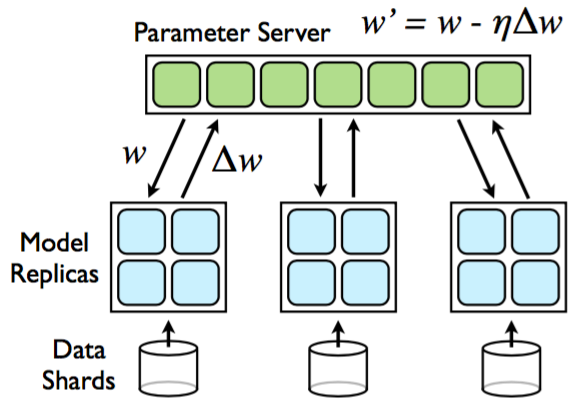
\includegraphics[width=0.6\textwidth]{figures/parameter-server.png}
\caption{DistBelief: Parameter Server架构}
 \label{fig:parameter-server}
\end{figure}

\end{content}

\subsubsection{缺陷与不足}

\begin{content}


但是,对于高级用户,\ascii{DistBelief}的编程模型,及其\ascii{Parameter Server}的系统架构,缺乏如下几个方面的扩展性。

\begin{enum}
  \eitem{优化算法:添加新的优化算法,必须修改\ascii{Parameter Server}的实现;\code{get(), put()}的抽象方法,对某些优化算法并不高效;}
  \eitem{训练算法:支持非前馈的神经网络具有很大的挑战性,例如包含循环的\ascii{RNN},交替训练的对抗网络,及其损失函数由分离的代理完成增强学习模型;} 
  \eitem{加速设备:\ascii{DistBelief}设计之初仅支持多核\ascii{CPU},并不支持\ascii{GPU};遗留的系统架构对支持新的计算设备缺乏弹性空间。}
\end{enum}

\end{content}

\subsection{今生:TensorFlow}

\begin{content}

正因为\ascii{DistBelief}遗留的架构和设计,不再满足潜在的深度学习与日俱增的需求,\ascii{Google}毅然决定在\ascii{DistBelief}基础上做全新的架构设计,从而诞生了\ascii{TensorFlow}。

\end{content}

\subsubsection{编程模型}

\begin{content}

\ascii{TensorFlow}使用数据流图\ascii{(Dataflow Graph)}表示计算过程和共享状态,使用节点表示抽象计算,使用边表示数据流。如\refig{tf-dataflow}所示,展示了\ascii{mnist}手写识别应用的数据流图。

在该模型中,前向子图使用了\ascii{2}层全连接网络,分别为\ascii{ReLU}层和\ascii{Softmax}层;随后,由\ascii{Gradients}构建了与前向子图对应的反向子图,用于训练参数的梯度计算;最后,使用`SGD`的优化算法,构造参数更新子图,完成参数的更新。

\begin{figure}[!htbp]
\centering
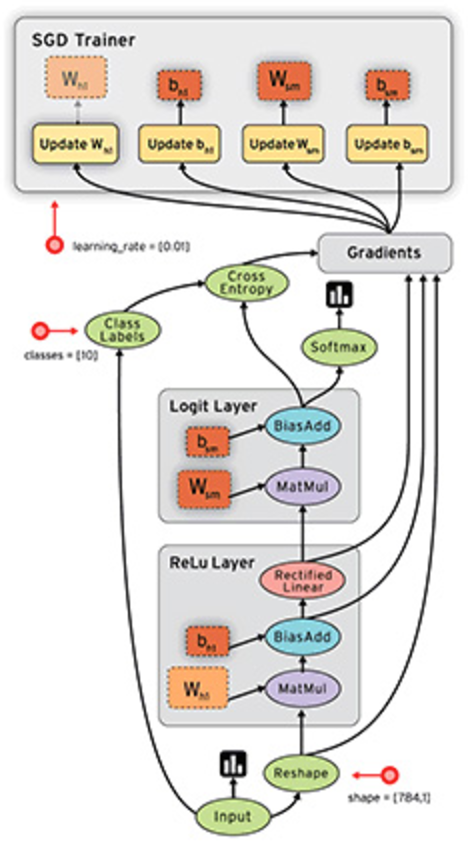
\includegraphics[width=0.4\textwidth]{figures/tf-dataflow.png}
\caption{TensorFlow数据流图}
 \label{fig:tf-dataflow}
\end{figure}

\end{content}

\subsubsection{设计原则}

\begin{content}

\begin{enum}
  \eitem{延迟计算:图的构造与执行分离,并推迟计算图的执行过程;}
  \eitem{原子\ascii{OP}:\ascii{OP}是最小的抽象计算单元,支持构造复杂的网络模型;} 
  \eitem{抽象设备:支持\ascii{CPU, GPU, TPU}多种异构计算设备类型;}
  \eitem{抽象任务:基于\ascii{Task}的\ascii{PS}任务,对新的优化算法和网络模型具有良好的可扩展性。}  
\end{enum}

\end{content}

\subsubsection{优势}

\begin{content}

相对于其他机器学习框架,\ascii{TensorFlow}具有如下方面的优势。

\begin{enum}
  \eitem{跨平台:支持多\ascii{CPU/GPU/TPU}运算;支持台式机/服务器/移动设备;支持\ascii{Windows,Linux,MacOS};}
  \eitem{分布式:支持本地和分布式的模型训练和推理;}
  \eitem{多语言:支持\ascii{Python, C++, Java, Go}等多种程序设计语言的\ascii{API};}  
  \eitem{通用性:支持各种复杂的网络模型的设计和实现;}
  \eitem{可扩展:支持\ascii{OP}扩展,\ascii{Kernel}扩展,\ascii{Device}扩展;}
  \eitem{可视化:使用\ascii{TensorBoard}可视化整个训练过程,包括计算图。}
\end{enum}

\end{content}

\section{社区发展}

\begin{content}

\tf{}是目前最为流行的机器学习框架。自开源以来,\tf{}社区相当活跃。来自众多的非\ascii{Google}员工拥有数万次代码提交,并且每周拥有近百个\ascii{Issue}被提交;在\ascii{Stack Overflow}上也拥有上万个关于\tf{}的问题被回答;在各类技术大会上,\tf{}也是一颗闪亮的明星,得到众多开发者的青睐。

\end{content}

\subsection{开源}

\begin{content}

\ascii{2015.11},\ascii{Google Research}发布文章:\href{https://research.googleblog.com/2015/11/tensorflow-googles-latest-machine\_9.html}{TensorFlow: Google's latest machine learning system, open sourced for everyone},正式宣布新一代机器学习系统\ascii{TensorFlow}开源。

随后,\ascii{TensorFlow}在\ascii{Github}上代码仓库短时间内获得了大量的\ascii{Star}和\ascii{Fork}。如\refig{tf-commits}所示,\ascii{TensorFlow}的社区活跃度已远远超过其他竞争对手,逐渐成为目前最为炙手可热的机器学习和深度学习框架,已然成为事实上的工业标准。

\begin{figure}[!htbp]
\centering
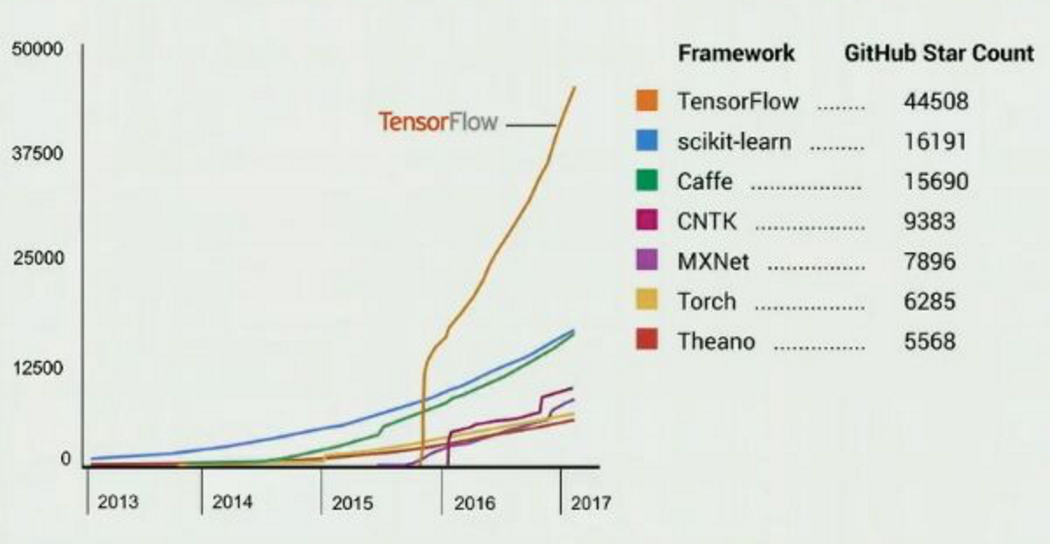
\includegraphics[width=1.0\textwidth]{figures/tf-commits.png}
\caption{TensorFlow社区活跃度}
 \label{fig:tf-commits}
\end{figure}

毫无疑问,\ascii{TensorFlow}的开源对学术界和工业界产生了巨大的影响,其极大地降低了深度学习在各个行业中应用的难度。众多的学者,工程师,企业,组织纷纷地投入到了\ascii{TensorFlow}社区,并一起完善和改进\ascii{TensorFlow},推动其不断地向前演进和发展。

\end{content}

\subsection{里程碑}

\begin{content}

\tf{}自\ascii{2015.11}开源依赖,平均一个多月发布一个版本。如\refig{tf-versions}所示,展示了\tf{}几个重要特性的发布时间。

\begin{figure}[!htbp]
\centering
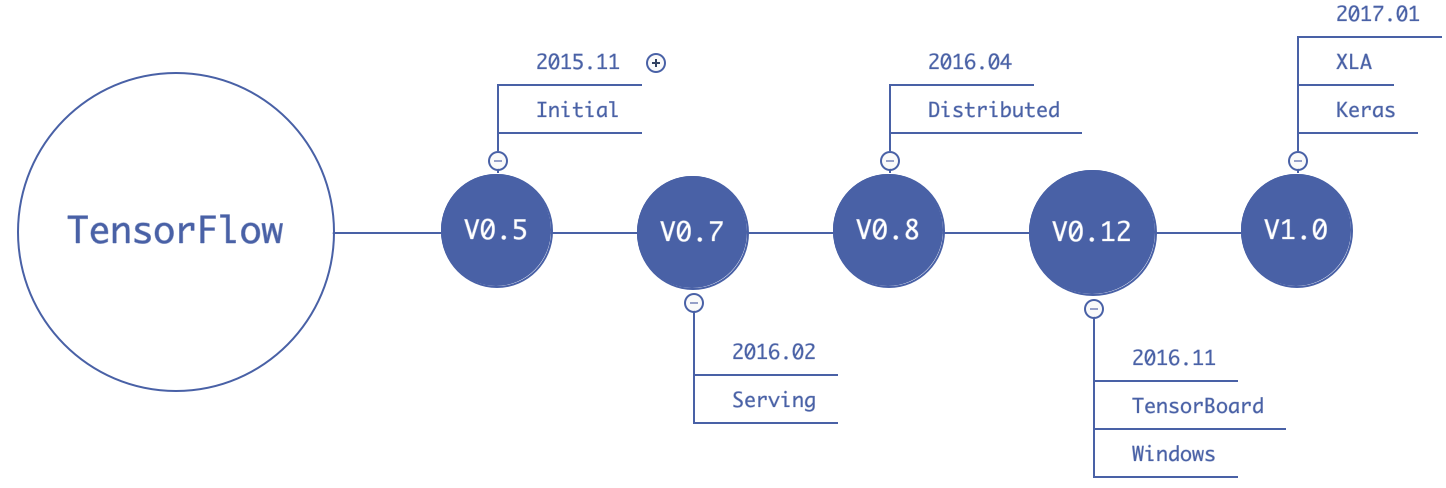
\includegraphics[width=1.0\textwidth]{figures/tf-versions.png}
\caption{TensorFlow重要里程碑}
 \label{fig:tf-versions}
\end{figure}

\end{content}

\subsection{工业应用}

\begin{content}

\ascii{TensorFlow}自开源发展一年多以来,在生产环境中被大量应用使用。在医疗方面,使用\ascii{TensorFlow}构建机器学习模型,帮助医生预测皮肤癌;在音乐、绘画领域,使用\ascii{TensorFlow}构建深度学习模型,帮助人类更好地理解艺术;在移动端,多款移动设备搭载\ascii{TensorFlow}训练的机器学习模型,用于翻译等工作。

如\refig{tf-google-apps}所示,\ascii{TensorFlow}在\ascii{Google}内部项目应用的增长也十分迅速,多个产品都有相关应用,包括:\ascii{Search, Gmail, Translate,  Maps}等等。

\begin{figure}[!htbp]
\centering
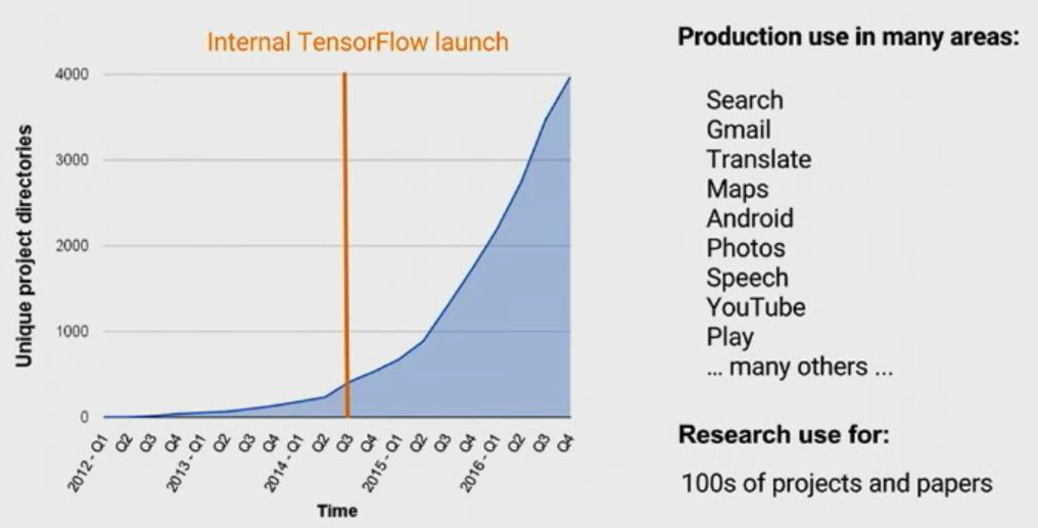
\includegraphics[width=1.0\textwidth]{figures/tf-google-apps.png}
\caption{TensorFlow在Google内部使用情况}
 \label{fig:tf-google-apps}
\end{figure}


\end{content}
\begin{savequote}[45mm]
\ascii{Any fool can write code that a computer can understand. Good programmers write code that humans can understand.}
\qauthor{\ascii{- Martin Flower}}
\end{savequote}

\chapter{编程环境} 
\label{ch:prog-env}

\begin{content}

为了实现\tf{}的快速入门,本章将介绍\tf{}的编程环境,包括代码结构,工程构建,以便对\tf{}的系统架构建立基本的感性认识。

\end{content}

\section{代码结构}

\begin{content}

\subsection{克隆源码}

首先,从\ascii{Github}上克隆\tf{}的源代码。


\begin{leftbar}
\begin{python}
$ git clone git@github.com:tensorflow/tensorflow.git
\end{python}
\end{leftbar}

然后,切换到最新的稳定分支上。例如,\code{r1.3}分支。

\begin{leftbar}
\begin{python}
$ cd tensorflow
$ git checkout r1.3
\end{python}
\end{leftbar}

\subsection{源码结构}

运行如下命令,打印出\tf{}源码的组织结构。

\begin{leftbar}
\begin{python}[]
$ tree -d -L 1 ./tensorflow
\end{python}
\end{leftbar}

其中,本书将重点关注\code{core, python}组件,部分涉及\code{c, cc, stream\_executor}组件。

\begin{leftbar}
\begin{c++}[caption={TensorFlow源码结构}]
./tensorflow
├── c
├── cc
├── compiler
├── contrib
├── core
├── docs_src
├── examples
├── g3doc
├── go
├── java
├── python
├── stream_executor
├── tools
└── user_ops
\end{c++}
\end{leftbar}

截止当前最新发布的\ascii{1.3}版本,\tf{}代码库拥有大约\ascii{100}万代码。其中,包括\ascii{53}万行\ascii{C/C++}代码,\ascii{37}万行\ascii{Python}代码,而且在不断膨胀之中。因此,可以推测\ascii{Python}提供的编程接口是最完善的;相比之下,其他编程语言尚处于起步阶段。

\begin{leftbar}
\begin{python}[caption={TensorFlow代码统计}]
-------------------------------------------------------
Language             files    blank    comment    code
-------------------------------------------------------
C++                   2238    77610     68275    443099
Python                1881    92018    151807    369399
C/C++ Header          1175    27392     46215     86691
Markdown               218     8859         2     30925
CMake                   50     2183       986     16398
Go                      28     1779     13290     15003
Java                    72     1789      3111      7779
Bourne Shell           103     1487      3105      6074
Protocol Buffers        87     1313      3339      3452
Objective C++            9      227       181      1201
C                        8      157       130       941
make                     4      105       136       612
XML                     25      135       265       315
Groovy                   3       46        74       246
Maven                    5       21         4       245
DOS Batch                9       30         0       143
Dockerfile               7       41        69       133
Perl                     2       29        38       130
Bourne Again Shell       3       24        63       111
JSON                     3        0         0        23
Objective C              1       10        13        21
YAML                     1        3        24        15
-------------------------------------------------------
SUM:                  5932   215258    291127    982956
-------------------------------------------------------
\end{python}
\end{leftbar}

\subsection{Core}

内核的源码结构如下所示,主要包括平台,实用函数库,基础框架,\ascii{Protobuf}定义,本地运行时,分布式运行时,图操作,\ascii{OP}定义,以及\ascii{Kernel}实现等组成,这是本书重点剖析的组件之一,将重点挖掘基础框架中隐藏的领域模型,追踪整个运行时环境的生命周期和图操作的详细过程,并揭示常见\ascii{OP}的\ascii{Kernel}实现原理和运行机制。

\begin{leftbar}
\begin{c++}[caption={Core源码结构}]
./tensorflow/core
├── common_runtime
├── debug
├── distributed_runtime
├── example
├── framework
├── graph
├── grappler
├── kernels
├── lib
├── ops
├── platform
├── profiler
├── protobuf
├── public
├── user_ops
└── util
\end{c++}
\end{leftbar}

其中,\code{core}主要由\code{C++}实现,大约拥有\ascii{26}万行代码。

\begin{leftbar}
\begin{python}[caption={Core代码统计}]
-------------------------------------------------------
Language             files    blank   comment      code
-------------------------------------------------------
C++                   1368    44791     38968    259289
C/C++ Header           653    15040     24474     50506
Protocol Buffers        57      736      2371      1806
Markdown                11      327         0      1285
JSON                     2        0         0        18
-------------------------------------------------------
SUM:                  2091    60894     65813    312904
-------------------------------------------------------
\end{python}
\end{leftbar}

\subsection{Python}

\ascii{Python}定义和实现了\tf{}的编程模型,并对外开放\ascii{API}供程序员使用,其源码结构如下所示,这也是本书重点剖析的对象。

\begin{leftbar}
\begin{c++}[caption={Python源码结构}]
./tensorflow/python
├── client
├── debug
├── estimator
├── feature_column
├── framework
├── grappler
├── kernel_tests
├── layers
├── lib
├── ops
├── platform
├── profiler
├── saved_model
├── summary
├── tools
├── training
├── user_ops
└── util
\end{c++}
\end{leftbar}

其中,该组件由\code{Python}实现,大约有\ascii{18}万行代码。

\begin{leftbar}
\begin{python}[caption={Python代码统计}]
-------------------------------------------------------
Language            files     blank   comment      code
-------------------------------------------------------
Python                714     45769     69407    179565
C++                    20       496       506      3658
C/C++ Header           15       207       387       363
Markdown                4        48         0       200
Protocol Buffers        3        16        10        71
Bourne Shell            1        13        28        68
-------------------------------------------------------
SUM:                  757     46549     70338    183925
-------------------------------------------------------
\end{python}
\end{leftbar}

\subsection{Contrib}

\code{contrib}是第三方贡献的编程库,它也是\tf{}标准化之前的实验性编程接口,犹如\ascii{Boost}社区与\ascii{C++}标准之间的关系。当\code{contrib}的接口成熟后,便会被\tf{}标准化,并从\code{contrib}中搬迁至\code{core, python}中,并正式对外发布\ascii{API}。

\begin{leftbar}
\begin{python}[caption={Contrib源码结构}]
./tensorflow/contrib
├── android
├── batching
├── bayesflow
├── benchmark_tools
├── boosted_trees
├── cloud
├── cluster_resolver
├── cmake
├── compiler
├── copy_graph
├── crf
├── cudnn_rnn
├── data
├── decision_trees
├── deprecated
├── distributions
├── eager
├── factorization
├── ffmpeg
├── framework
├── fused_conv
├── gdr
├── graph_editor
├── grid_rnn
├── hooks
├── hvx
├── image
├── imperative
├── input_pipeline
├── integrate
├── keras
├── kernel_methods
├── labeled_tensor
├── layers
├── learn
├── legacy_seq2seq
├── linalg
├── linear_optimizer
├── lookup
├── losses
├── makefile
├── memory_stats
├── meta_graph_transform
├── metrics
├── mpi
├── nccl
├── ndlstm
├── nearest_neighbor
├── nn
├── opt
├── pi_examples
├── predictor
├── quantization
├── reduce_slice_ops
├── remote_fused_graph
├── resampler
├── rnn
├── saved_model
├── seq2seq
├── session_bundle
├── signal
├── slim
├── solvers
├── sparsemax
├── specs
├── staging
├── stat_summarizer
├── stateless
├── tensor_forest
├── tensorboard
├── testing
├── text
├── tfprof
├── timeseries
├── tpu
├── training
├── util
├── verbs
└── xla_tf_graph
\end{python}
\end{leftbar}

由于\tf{}社区相当活跃,\code{contrib}的变更相当频繁,截止\ascii{1.3}版本,大约有\ascii{23}万行代码,主要由\ascii{Python}设计和实现的编程接口,部分运行时由\ascii{C++}实现。

\begin{leftbar}
\begin{python}[caption={Contrib代码统计}]
-------------------------------------------------------
Language            files     blank   comment      code
-------------------------------------------------------
Python               1007     41436     75096    170355
C++                   201      5500      5313     32944
CMake                  48      2172       955     16358
C/C++ Header           99      1875      2867      6583
Markdown               46      1108         0      3485
Bourne Shell           18       232       386      1272
C                       7       151       118       931
Protocol Buffers       20       224       454       680
make                    4       105       136       612
Java                    2        77       209       335
Groovy                  1        10        20        75
Bourne Again Shell      1         6        15        59
Dockerfile              1         2         1        14
XML                     2         3         0         9
-------------------------------------------------------
SUM:                 1457     52901     85570    233712
-------------------------------------------------------
\end{python}
\end{leftbar}

\subsection{StreamExecutor}

\ascii{StreamExecutor}是\ascii{Google}另一个开源组件库,它提供了主机端(\ascii{host-side})的编程模型和运行时环境,实现了对\ascii{CUDA}和\ascii{OpenCL}的统一封装。使得主机端的代码中,可以将功能相同、数据并行的内核函数无缝地部署在\code{CUDA}或\code{OpenCL}的计算设备上执行。

目前,\ascii{StreamExecutor}被大量应用于\ascii{Google}内部的\ascii{GPGPU}应用程序的运行时。其中,\tf{}运行时也包含了一个\ascii{StreamExecutor}的快照版本,用于封装\ascii{CUDA}和\code{OpenCL}的运行时,本书将简单介绍\ascii{CUDA}的编程模型和线程模型,并详细介绍\ascii{StreamExecutor}的系统架构与工作原理,揭示\ascii{Kernel}一般的实现模式和习惯用法。

\begin{leftbar}
\begin{c++}[caption={StreamExecutor源码结构}]
./tensorflow/stream_executor
├── cuda
├── host
├── lib
└── platform
\end{c++}
\end{leftbar}

其中,\ascii{StreamExecutor}使用\code{C++}实现,大约有\ascii{2.5}万行代码。

\begin{leftbar}
\begin{python}[caption={StreamExecutor代码统计}]
-------------------------------------------------------
Language            files     blank   comment      code
-------------------------------------------------------
C++                    43      2440      1196     16577
C/C++ Header           81      2322      5080      8625
-------------------------------------------------------
SUM:                  124      4762      6276     25202
-------------------------------------------------------
\end{python}
\end{leftbar}

\subsection{Compiler}

众所周知,灵活性是\tf{}最重要的设计目标和核心优势,因此\tf{}的系统架构具有良好的可扩展性。\tf{}可用于定义任意图结构,并使用异构的计算设备有效地执行。但是,熊掌与鱼翅不可兼得,当低级\code{OP}组合为计算子图时,并期望在\code{GPU}上有效执行时,运行时将启动更多的\code{Kernel}的运算。

因此,\tf{}分解和组合\code{OP}的方法,在运行时并不能保证以最有效的方式运行。此时,\ascii{XLA}技术孕育而生,它使用\ascii{JIT}编译技术来分析运行时的计算图,它将多个\code{OP}融合在一起,并生成更高效的本地机器代码,提升计算图的执行效率。

\begin{leftbar}
\begin{python}[caption={Compiler源码结构}]
./tensorflow/compiler
├── aot
├── jit
├── plugin
├── tests
├── tf2xla
└── xla
\end{python}
\end{leftbar}

\ascii{XLA}技术目前处于初级的研发阶段,是\tf{}社区较为活跃研究方向,截止目前代码规模大约为\ascii{12.5}万行,主要使用\ascii{C++}实现。

\begin{leftbar}
\begin{python}[caption={Compiler代码统计}]
-------------------------------------------------------
Language            files     blank   comment      code
-------------------------------------------------------
C++                   455     19010     18334    102537
C/C++ Header          250      5939     10323     15510
Python                 37      1255      1416      6446
Protocol Buffers        5       312       501       781
Markdown                2         0         0         3
-------------------------------------------------------
SUM:                  749     26516     30574    125277
-------------------------------------------------------
\end{python}
\end{leftbar}

\end{content}

\section{工程构建}

\begin{content}

在开始之前,尝试\tf{}源码的构建过程,了解\tf{}的基本构建方式、工具,及其依赖的组件库、及其第三方工具包,对于理解\tf{}工作原理具有很大的帮助。但是,因篇幅受限,本章仅以\ascii{Mac OS}为例,讲述\tf{}的源码编译、安装、及其验证过程。其他操作系统,请查阅\tf{}的官方文档。

\subsection{环境准备}

\ascii{TensorFlow}的前端是一个支持多语言的编程接口。因此,编译\ascii{TensorFlow}源代码之前,需要事先安装相关的编译器、解释器、及其运行时环境。例如,使用\ascii{Python}作为编程接口,需要事先安装\ascii{Python}解释器。

其次,在构建系统之前,也需要事先安装\ascii{GCC}或\ascii{Clang}等\ascii{C++}编译器,用于编译后端系统实现。另外,\ascii{TensorFlow}使用\ascii{Bazel}的构建工具,是一个更高抽象的\ascii{Make}工具。不幸的是,\ascii{Bazel}依赖于\ascii{JDK},因此在安装\ascii{Bazel}之前,还得需要事先安装\ascii{JDK}。

\subsubsection{安装JDK}

推荐从\ascii{Oracle}官网上下载\ascii{1.8}及以上版本的\ascii{JDK},然后配置相关环境变量。

\begin{leftbar}
\begin{python}
$ sudo mkdir -p /usr/lib/jvm
$ sudo tar zxvf jdk-8u51-linux-x64.tar.gz -C /usr/lib/jvm
$ sudo ln -s /usr/java/jdk1.8.0_51 /usr/java/default
\end{python}
\end{leftbar}

创建\ascii{Java}相关的环境变量,并将其添加到\code{~/.bashrc}的配置文件中。

\begin{leftbar}
\begin{python}
$ echo 'export JAVA_HOME=/usr/java/default' >> ~/.bashrc
$ echo 'export PATH="$JAVA_HOME/bin:$PATH"' >> ~/.bashrc
\end{python}
\end{leftbar}

\subsubsection{安装Bazel}

在\ascii{Mac OS}上,可以使用\ascii{brew}安装\ascii{Bazel}。

\begin{leftbar}
\begin{python}
$ brew install bazel
\end{python}
\end{leftbar}

如果系统未安装\ascii{brew},可以执行如下命令先安装\ascii{brew}。当然,安装\ascii{brew}需要事先安装\ascii{Ruby}解释器,在此不再冗述。

\begin{leftbar}
\begin{python}
$ /usr/bin/ruby -e "$(curl -fsSL https://raw.githubusercontent.com/Homebrew/install/master/install)"
\end{python}
\end{leftbar}

\subsubsection{安装Swig}

\ascii{TensorFlow}使用\ascii{Swig}构建多语言的编程环境,自动生成相关的包装器。因此,在构建之前需要事先安装\ascii{Swig}的工具包。

\begin{leftbar}
\begin{python}
$ brew install swig
\end{python}
\end{leftbar}

\subsubsection{安装Python依赖包}

使用\ascii{pip}安装\ascii{TensorFlow}所依赖的\ascii{Python}包。

\begin{leftbar}
\begin{python}
$ sudo pip install six numpy wheel autograd
\end{python}
\end{leftbar}

如果系统未安装\ascii{pip},则可以使用\ascii{brew}先安装\ascii{pip}。

\begin{leftbar}
\begin{python}
$ brew install pip
\end{python}
\end{leftbar}

\subsubsection{安装CUDA工具包}

当系统安装了\ascii{CUDA}计算兼容性大于或等于\ascii{3.0}的\ascii{GPU}卡时,则需要安装\ascii{CUDA工具包, cuDNN},实现\tf{}运行时的\ascii{GPU}加速。推荐从\ascii{NVIDIA}官网上下载\ascii{CUDA Toolkit 8}及以上版本,并安装到系统中,配置相关环境变量。

\begin{leftbar}
\begin{python}
$ echo 'export CUDA_HOME=/usr/local/cuda' >> ~/.bashrc
$ echo 'export LD_LIBRARY_PATH=$CUDA_HOME/lib:$LD_LIBRARY_PATH' >> ~/.bashrc
\end{python}
\end{leftbar}

然后,再下载\ascii{cuDNN 5.1}及以上版本,并将其解压至\code{CUDA\_HOME}相关系统目录中。

\begin{leftbar}
\begin{python}
$ sudo tar -xvf cudnn-8.0-macos-x64-v5.1.tgz -C /usr/local
\end{python}
\end{leftbar}

\subsection{配置}

至此,编译环境一切就绪,执行\code{./configure}配置\ascii{TensorFlow}的编译环境了。特殊地,当系统支持\ascii{GPU},则需要配置相关的\ascii{CUDA/cuDNN}编译环境。

\begin{leftbar}
\begin{python}
$ ./configure
\end{python}
\end{leftbar}

\subsection{构建}

当配置成功后,使用\ascii{Bazel}启动\ascii{TensorFlow}的编译。

\begin{leftbar}
\begin{python}
$ bazel build --config=opt //tensorflow/tools/pip_package:build_pip_package
\end{python}
\end{leftbar}

特殊地,当支持\ascii{GPU}计算时,添加\code{--config=cuda}编译选项。

\begin{leftbar}
\begin{python}
$ bazel build -c opt --config=cuda //tensorflow/tools/pip_package:build_pip_package
\end{python}
\end{leftbar}

编译成功后,便可以构建\ascii{TensorFlow}的\ascii{Wheel}包。

\begin{leftbar}
\begin{python}
$ bazel-bin/tensorflow/tools/pip_package/build_pip_package /tmp/tensorflow_pkg
\end{python}
\end{leftbar}

\subsection{安装}

当\ascii{Whell}包构建成功后,使用\ascii{pip}安装\ascii{TensorFlow}到系统中。

\begin{leftbar}
\begin{python}
$ sudo pip install /tmp/tensorflow_pkg/tensorflow-1.2.0-py2-none-any.whl
\end{python}
\end{leftbar}

\subsection{验证}

启动\ascii{Python}解释器,验证\ascii{TensorFlow}安装是否成功。

\begin{leftbar}
\begin{python}
$ python
>>> import tensorflow as tf
>>> hello = tf.constant('Hello, TensorFlow!')
>>> sess = tf.Session()
>>> print(sess.run(hello))
Hello, TensorFlow!
\end{python}
\end{leftbar}

\subsection{配置IDE}

在阅读代码之前,选择一个适宜的\ascii{IDE}可以改善代码阅读的质量和速度。作者推荐使用\ascii{Eclipse CDT}阅读\ascii{C++}代码,使用\ascii{PyCharm}阅读\ascii{Python}代码。当阅读\code{Python}时,导入\tf{}源代码到\ascii{PyCharm}即可,在此不再冗述。但是,当阅读\ascii{C++}代码时,需要配置\ascii{TensorFlow, CUDA, Eigen3}头文件的搜索目录,并添加相关预定义的宏,以便\code{CDT}正确解析代码中的符号。

\subsubsection{创建Eclipse工程}

创建一个\ascii{Eclipse C++}工程,如\refig{setup-eclipse}所示。确定唯一的项目名称,手动地指定\ascii{TensorFlow}源代码的根目录,并选择\ascii{Makefile}的空工程。然后,按照\ascii{Properties > C/C++ General > Paths and Symbols > Includes}配置头文件的搜索目录。

\begin{table}[!htbl]
\resizebox{0.95\textwidth}{!} {
\begin{tabular*}{1.2\textwidth}{@{}ll@{}}
\toprule
\ascii{配置项} & \ascii{目录} \\
\midrule
\ascii{TensorFlow} & \code{/usr/local/lib/python2.7/site-packages/tensorflow/include} \\
\ascii{CUDA} & \code{/usr/local/cuda/include} \\ 
\bottomrule
\end{tabular*}
}
\caption{头文件搜索目录}
\label{tbl:tf-includes}
\end{table}

\begin{figure}[!htbl]
\centering
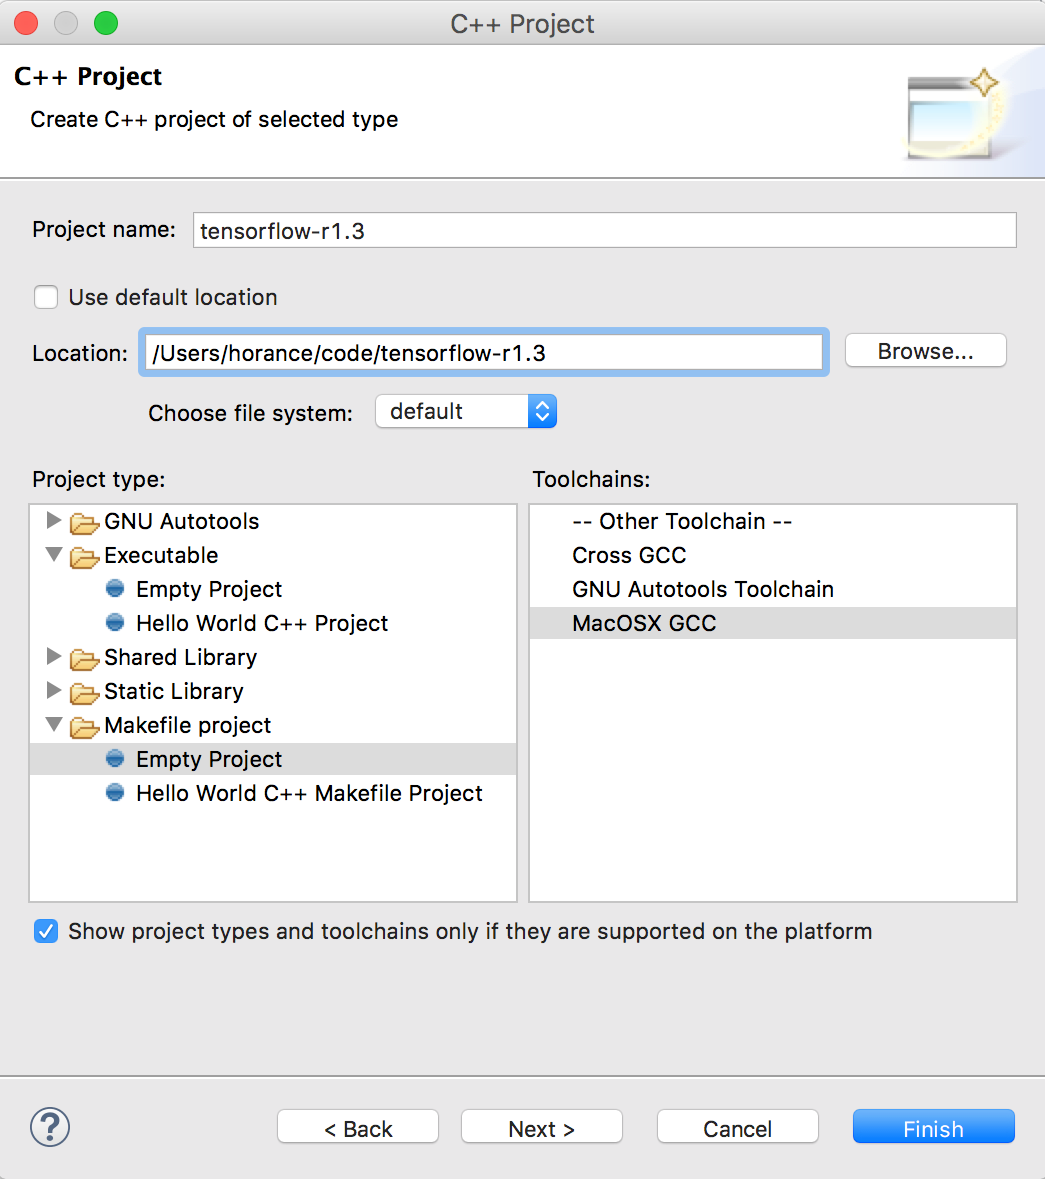
\includegraphics[width=0.75\textwidth]{figures/setup-eclipse.png}
\caption{创建Eclipse C++工程}}
 \label{fig:setup-eclipse}
\end{figure}

\subsubsection{配置Eigen}

不幸的是,\ascii{Eigen}对外公开的头文件缺少\code{.h}的后缀名,\code{CDT}无法解析相关的符号。请参阅\code{\href{http://eigen.tuxfamily.org/index.php?title=IDEs}{http://eigen.tuxfamily.org/index.php?title=IDEs}}相关说明,按照\ascii{Preferences > C/C++ > Coding Style > Organize Includes > Header Substitution}导入\code{eigen-header-substitution.xml}文件,如\refig{eclipse-eigen3}所示。

\begin{figure}[!htbl]
\centering
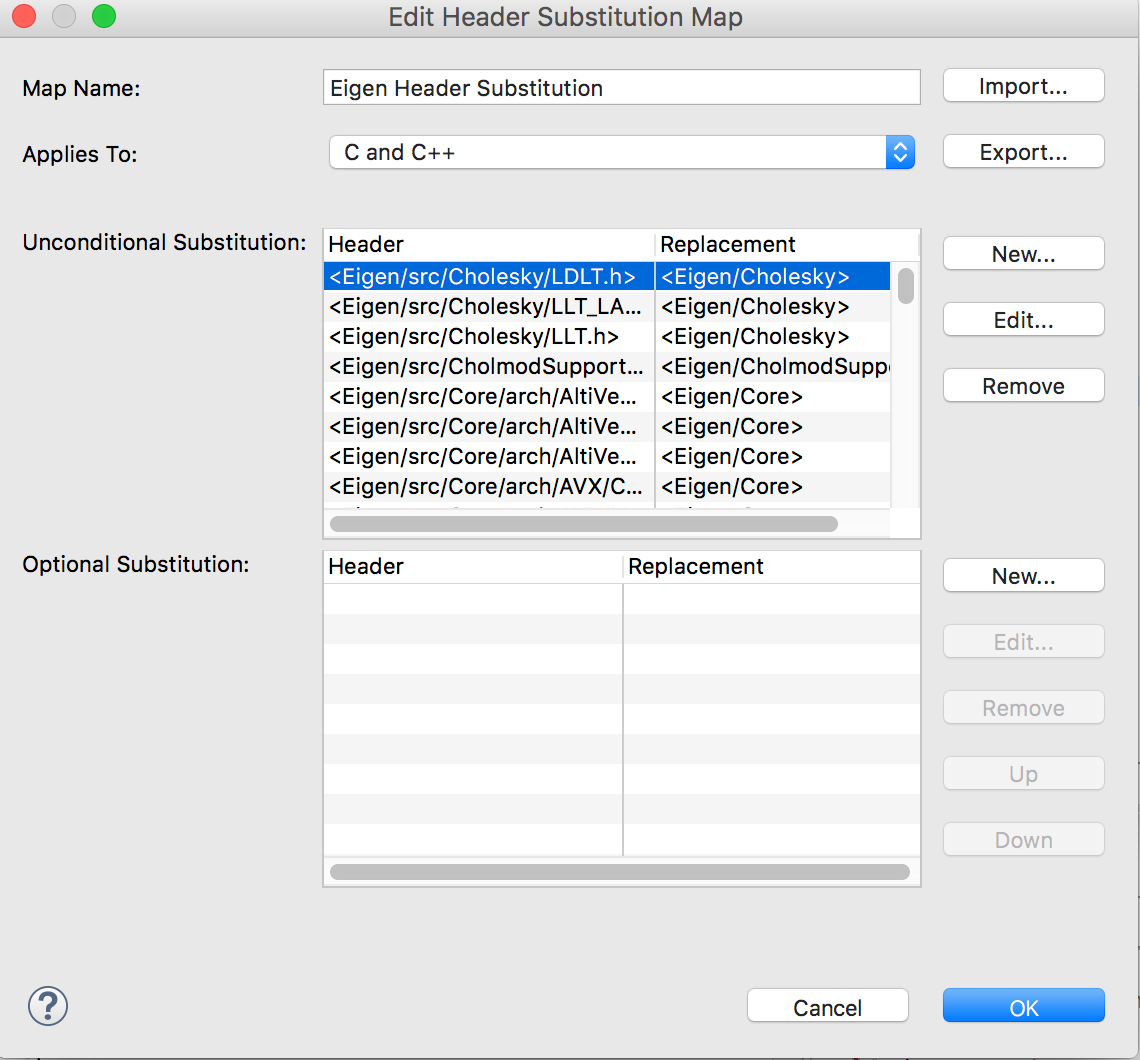
\includegraphics[width=0.75\textwidth]{figures/eclipse-eigen3.png}
\caption{替换\ascii{Eigen}的头文件}
 \label{fig:eclipse-eigen3}
\end{figure}

\end{content}

\section{技术栈}

\begin{content}

如\refig{tf-stack}所示,按照系统的层次结构展示了\tf{}的技术栈,构成了\tf{}生态系统的核心。

\begin{figure}[H]
\centering
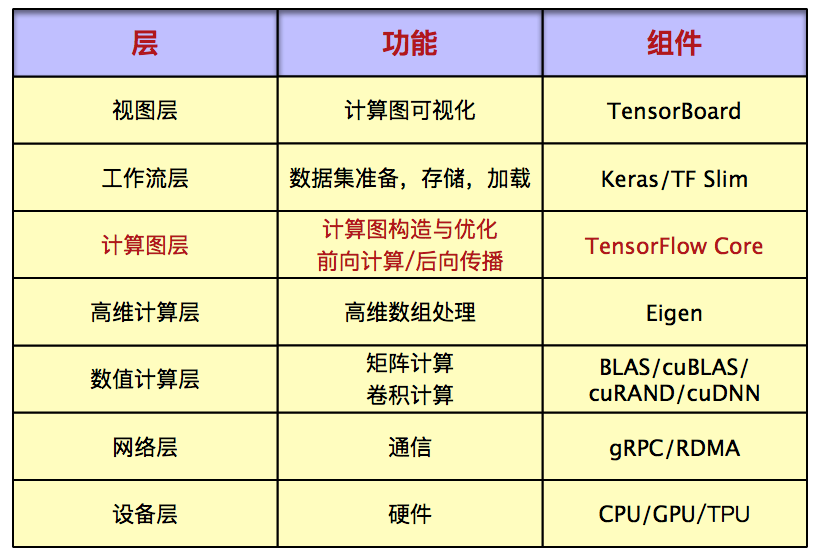
\includegraphics[width=0.7\textwidth]{figures/tf-stack.png}
\caption{TensorFlow技术栈}}
 \label{fig:tf-stack}
\end{figure}

\end{content}

\begin{savequote}[45mm]
\ascii{Any fool can write code that a computer can understand. Good programmers write code that humans can understand.}
\qauthor{\ascii{- Martin Flower}}
\end{savequote}

\chapter{系统架构} 
\label{ch:architecture}

\begin{content}

本章将阐述\tf{}的系统架构,并一个简单的例子,讲述图结构的变换过程,加深理解\tf{}运行时的工作机理。

\end{content}

\section{系统架构}

\begin{content}

\tf{}的系统结构以\ascii{C API}为界,将整个系统分为「前端」和「后端」两个子系统:

\begin{enum}
  \eitem{前端系统:提供编程模型,负责构造计算图;}
  \eitem{后端系统:提供运行时环境,负责执行计算图。} 
\end{enum}

\begin{figure}[!htbp]
\centering
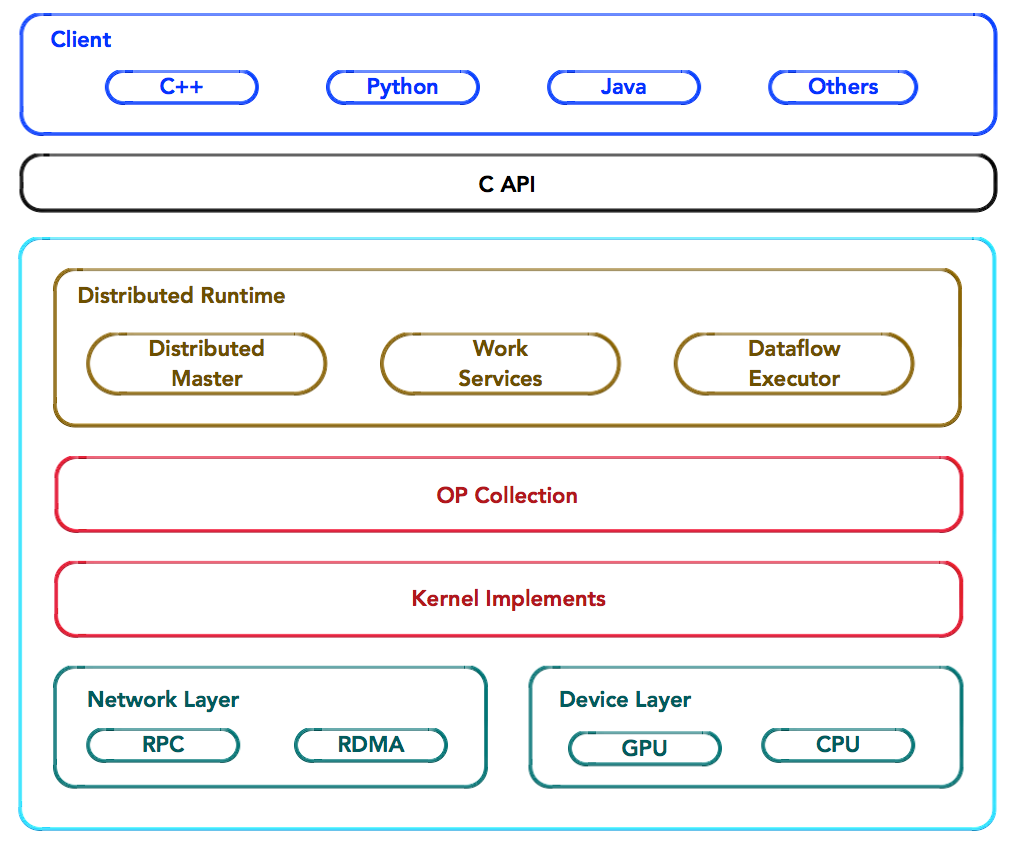
\includegraphics[width=0.9\textwidth]{figures/tf-architecture.png}
\caption{TensorFlow系统架构}
 \label{fig:tf-architecture}
\end{figure}

如\refig{tf-architecture}所示,重点关注系统中如下\ascii{4}个基本组件,它们是系统分布式运行时的核心。

\subsection{Client}

\ascii{Client}是前端系统的主要组成部分,它是一个支持多语言的编程环境。\ascii{Client}基于\ascii{TensorFlow}的编程接口,构造计算图。目前,\ascii{TensorFlow}支持\ascii{Python}和\ascii{C++}的编程接口较为完善,尤其对\ascii{Python}支持最佳;并且,对其他编程语言的编程接口的支持日益完善。

此时,\ascii{TensorFlow}并未执行任何的图计算,直至与后台计算引擎建立\ascii{Session},并以\ascii{Session}为桥梁,建立\ascii{Client}与\ascii{Master}之间的通道,将\ascii{Protobuf}格式的\ascii{GraphDef}发送至\ascii{Master},启动计算图的执行过程。

\subsection{Master}

在分布式的运行时环境中,\ascii{Client}根据\code{Session.run}传递整个计算图给后端的\ascii{Master};此时,计算图是完整的,常称为\ascii{Full Graph}。

随后,\ascii{Master}根据\ascii{Client}通过\code{Session.run}传递\code{fetches}参数列表,反向遍历\ascii{Full Graph},并按照依赖关系,对其实施剪枝,最终计算得到所依赖的「最小子图」,常称为\ascii{Client Graph}。

随后,\ascii{Master}负责将\ascii{Client Graph}按照任务的名称分裂\ascii{(split-by-task)}为多个「子图片段」,常称为\ascii{(Graph Partition)};其中,每个\ascii{Worker}对应一个\ascii{Graph Partition}。

随后,\ascii{Master}将\ascii{Graph Partition}分别注册到相应的\ascii{Worker}上,以便在不同的\ascii{Worker}上并发执行这些「子图片段」。

最后,\ascii{Master}将通知所有\ascii{Work}启动相应的\ascii{Graph Partition}的执行;其中,\ascii{Work}之间可能存在数据交互,\ascii{Master}不参与两者之间的数据交换,它们自行通信,独立交换数据即可,直至计算完成。

\subsection{Worker}

对于每以个任务,\tf{}都将启动一个\ascii{Worker}实例。\ascii{Worker}主要负责如下\ascii{3}个方面的职责:

\begin{enum}
  \eitem{处理来自\ascii{Master}的请求;}
  \eitem{调度\ascii{OP}的\ascii{Kernel}实现,执行本地子图;} 
  \eitem{协同任务之间的数据通信。}
\end{enum}

首先,\ascii{Worker}收到\ascii{Master}发送过来的图执行命令,此时的计算图相对于\ascii{Worker}是完整的,也称为\ascii{Full Graph},它对应于\ascii{Master}的一个\ascii{Graph Partition}。随后,\ascii{Worker}也会执行图剪枝,得到最小依赖的\ascii{Client Graph}。

随后,\ascii{Worker}根据当前可用的硬件环境,包括\ascii{(GPU/CPU)}资源,按照\ascii{OP}设备的约束规范,再将\ascii{Cliet Graph}分裂\ascii{(split-by-device)}为多个\ascii{Graph Partition};其中,每个计算设备对应一个\ascii{Graph Partition};随后,\ascii{Worker}启动所有当前设备的\ascii{Graph Partition}的执行。

最后,对于每一个计算设备,\ascii{Worker}将按照计算图中节点之间的依赖关系执行拓扑排序算法,并依次调用\ascii{OP}的\ascii{Kernel}实现,完成\ascii{OP}的运算(一种典型的多态实现技术)。其中,\ascii{Worker}还要负责将\ascii{OP}运算的结果发送到其他的\ascii{Work};或者接受来自其他\ascii{Worker}发送给它运算的结果,以便实现\ascii{Worker}之间的数据交互。

\subsection{Kernel}

\ascii{Kernel}是\ascii{OP}在某种硬件设备的特定实现,它负责执行\ascii{OP}的具体运算。目前,\ascii{TensorFlow}系统中包含\ascii{200}多个标准的\ascii{OP},包括数值计算,多维数组操作,控制流,状态管理等。

每一个\ascii{OP}根据设备类型都会存在一个优化了的\ascii{Kernel}实现。在运行时,运行时根据\ascii{OP}的设备约束贵方,及其本地设备的类型,为\ascii{OP}选择特定的\ascii{Kernel}实现,完成该\ascii{OP}的计算。

其中,大多数\ascii{Kernel}基于\ascii{Eigen::Tensor}实现。其中,\ascii{Eigen::Tensor}是一个使用\ascii{C++}模板技术,为多核\ascii{CPU/GPU}生成高效的并发代码。但是,\ascii{TensorFlow}也可以灵活地直接使用\ascii{cuDNN}实现更高效的\ascii{Kernel}。

此外,\ascii{TensorFlow}实现了矢量化技术,在高吞吐量、以数据为中心的应用需求中,及其移动设备中,实现更高效的推理。如果对于复合\ascii{OP}的子计算过程很难表示,或执行效率低下,\ascii{TensorFlow}甚至支持更高效的\ascii{Kernel}注册,其扩展性表现相当优越。

\end{content}

\section{图控制}

\begin{content}

随后,通过一个最简单的例子,进一步抽丝剥茧,逐渐挖掘出\tf{}计算图的控制与运行机制。


\subsection{组建集群}

如\refig{tf-1ps-1worker}所示。假如存在一个简单的分布式环境:\ascii{1 PS + 1 Worker},并将其划分为两个任务:

\begin{enum}
  \eitem{\ascii{ps0}: 使用\code{/job:ps/task:0}标记,负责模型参数的存储和更新;}
  \eitem{\ascii{worker0}: \code{/job:worker/task:0}标记,负责模型的训练。} 
\end{enum}

\begin{figure}[!htbp]
\centering
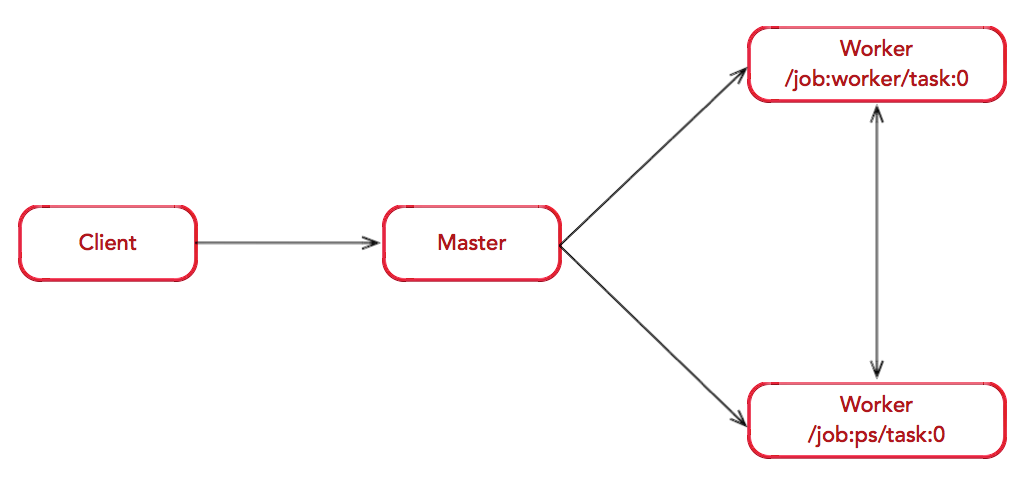
\includegraphics[width=0.9\textwidth]{figures/tf-1ps-1worker.png}
\caption{TensorFlow集群:\ascii{1 PS + 1 Worker}}
 \label{fig:tf-1ps-1worker}
\end{figure}

\subsection{图构造}

如\refig{tf-graph-construction}所示。\ascii{Client}构建了一个简单计算图;首先,将$w$与$x$进行矩阵相乘,再与截距$b$按位相加,最后更新至$s$。

\begin{figure}[!htbp]
\centering
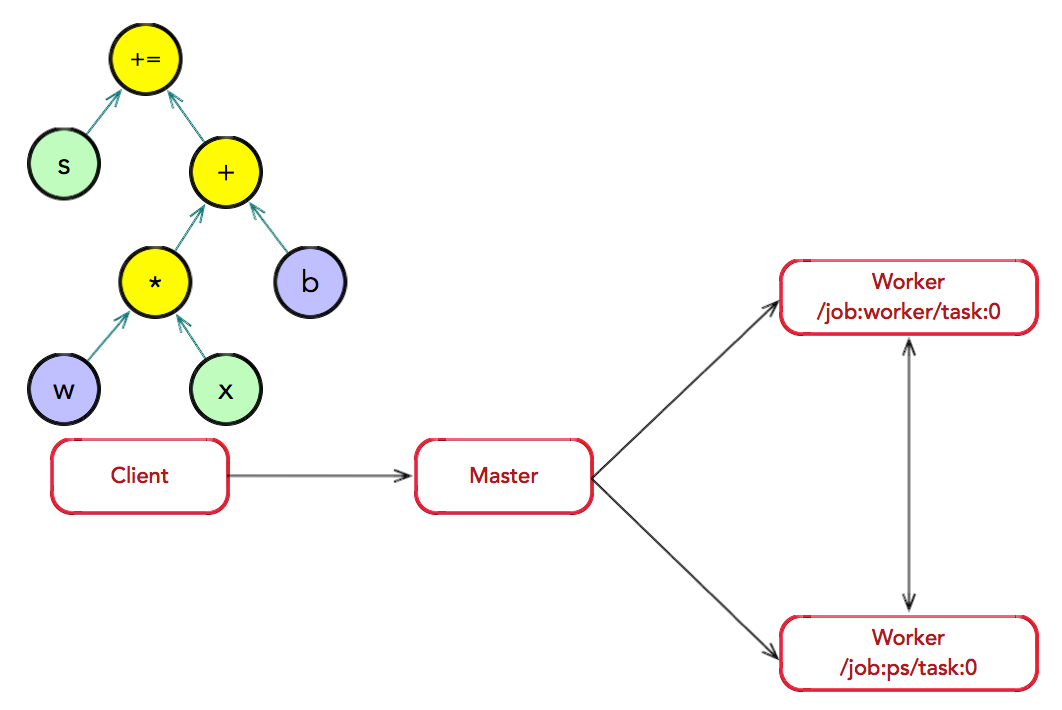
\includegraphics[width=0.9\textwidth]{figures/tf-graph-construction.png}
\caption{图构造}}
 \label{fig:tf-graph-construction}
\end{figure}

\subsection{图执行}

如\refig{tf-graph-execution}所示。首先,\ascii{Client}创建一个\code{Session}实例,建立与\ascii{Master}之间的通道;接着,\ascii{Client}通过调用\code{Sess.run}将计算图传递给\ascii{Master}。

随后,\ascii{Master}便开始启动一次\ascii{Step}的图计算过程。在执行之前,\ascii{Master}会实施一系列优化技术,例如「公共表达式消除」,「常量折叠」等。最后,\ascii{Master}负责任务之间的协同,执行优化后的计算子图。

\begin{figure}[!htbp]
\centering
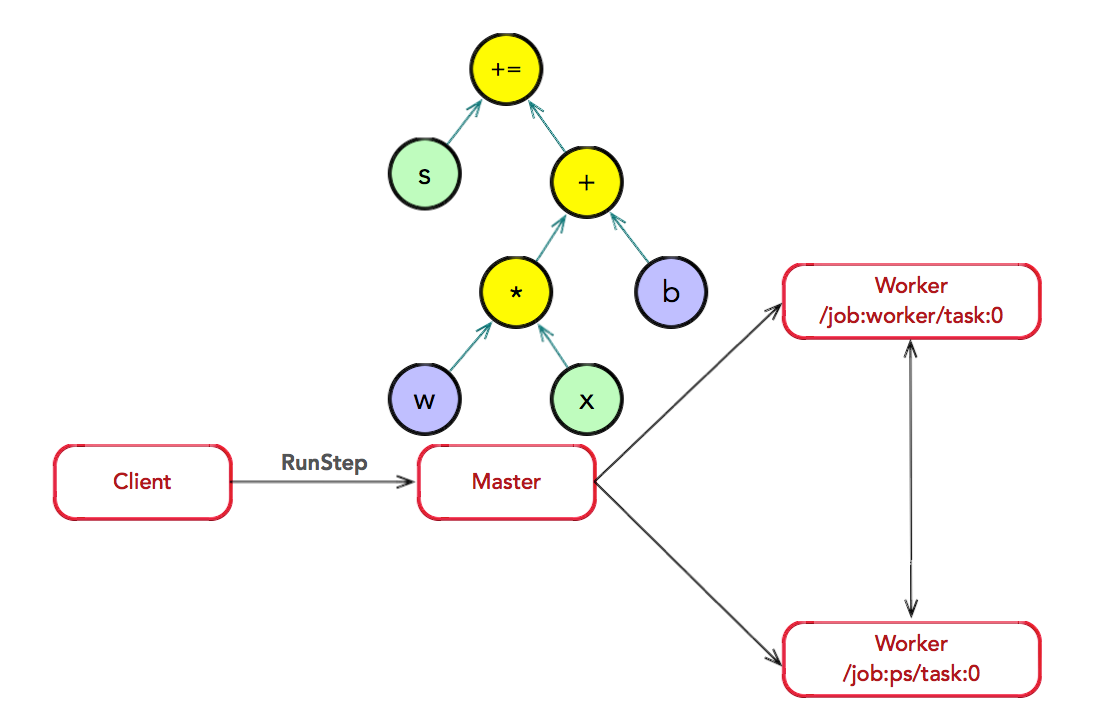
\includegraphics[width=0.9\textwidth]{figures/tf-graph-execution.png}
\caption{图执行}}
 \label{fig:tf-graph-execution}
\end{figure}

\subsubsection{图分裂}

如\refig{tf-graph-split-by-task}所示。存在一种合理的图划分算法。\ascii{Master}将模型参数相关的\ascii{OP}划分为一组,并放置在\ascii{ps0}任务上;其他\ascii{OP}划分为另外一组,放置在\ascii{worker0}任务上执行。

\begin{figure}[!htbp]
\centering
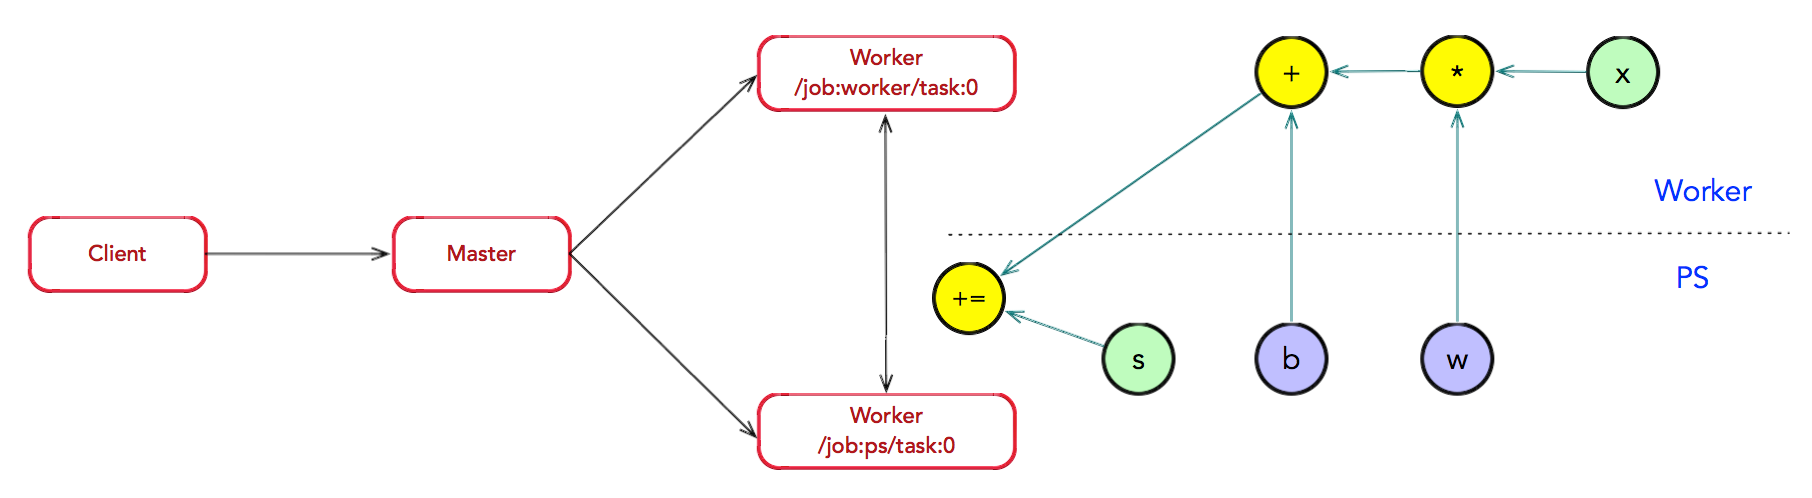
\includegraphics[width=0.9\textwidth]{figures/tf-graph-split-by-task.png}
\caption{图分裂:按任务划分}}
 \label{fig:tf-graph-split-by-task}
\end{figure}

\subsubsection{子图注册}

如\refig{tf-register-graph}所示。在图分离过程中,如果计算图的边跨越任务节点,\ascii{Master}将该边进行分裂,在两个任务之间插入\ascii{Send}和\ascii{Recv}节点,实现数据的传递。

其中,\ascii{Send}和\ascii{Recv}节点也是\ascii{OP},这是两个特殊的\ascii{OP},由内部运行时管理和控制,对用户不可见;并且,它们仅用于数据的通信,并没有任何数据计算的逻辑。

最后,\ascii{Master}通过调用\code{RegisterGraph}接口,将\ascii{Graph Partition}注册给相应的任务中,并由相应的\ascii{Worker}负责执行。

\begin{figure}[!htbp]
\centering
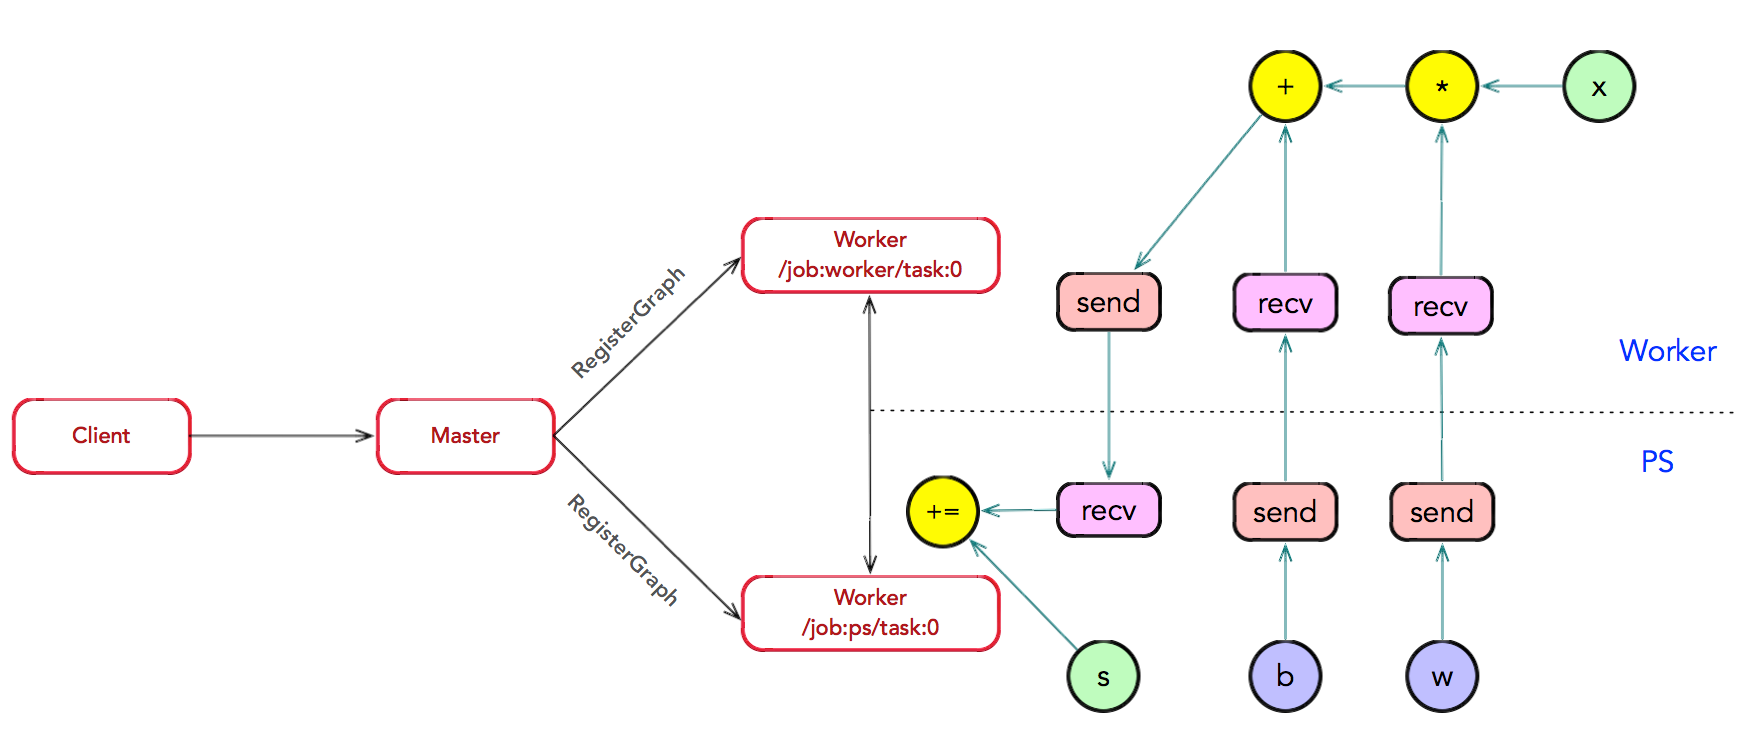
\includegraphics[width=0.9\textwidth]{figures/tf-register-graph.png}
\caption{子图注册:插入Send和Recv节点}}
 \label{fig:tf-register-graph}
\end{figure}

\subsubsection{子图运算}

如\refig{tf-run-graph}所示。\ascii{Master}通过调用\code{RunGraph}接口,通知所有\ascii{Worker}执行子图运算。其中,\ascii{Worker}之间通过调用\code{RecvTensor}接口,完成数据的交互。

\begin{figure}[!htbp]
\centering
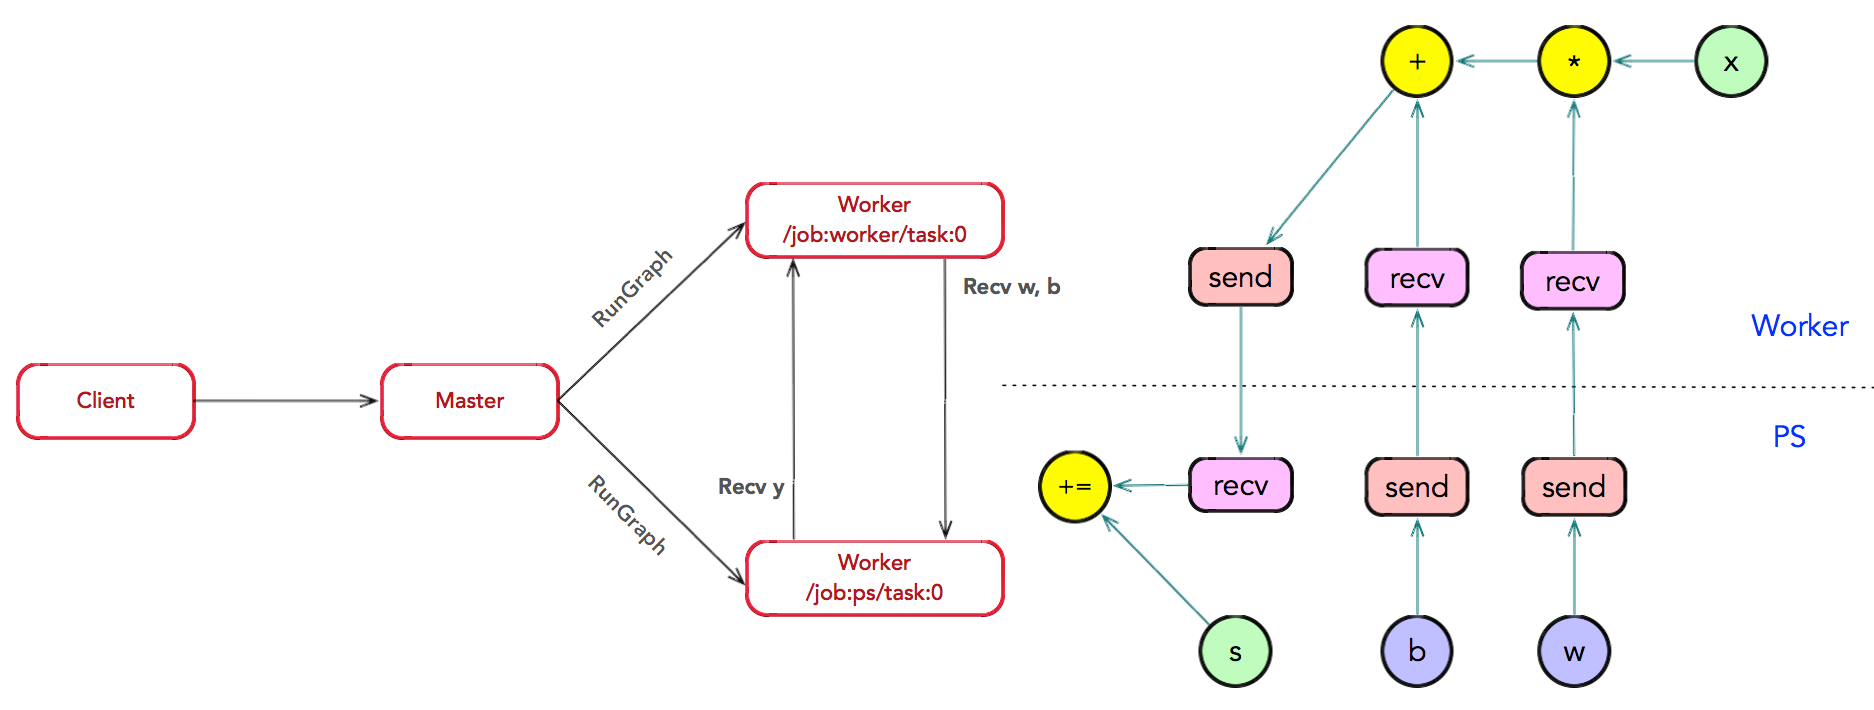
\includegraphics[width=0.9\textwidth]{figures/tf-run-graph.png}
\caption{子图执行}}
 \label{fig:tf-run-graph}
\end{figure}

\end{content}













\begin{savequote}[45mm]
\ascii{Any fool can write code that a computer can understand. Good programmers write code that humans can understand.}
\qauthor{\ascii{- Martin Flower}}
\end{savequote}

\chapter{计算图} 
\label{ch:computation-graph}

\begin{content}

在\tf{}的计算图中,使用\ascii{OP}表示节点,根据\ascii{OP}之间计算和数据依赖关系,构造\ascii{OP}之间生产与消费的数据依赖关系,并通过有向边表示。

其中,有向边存在两种类型,一种承载数据,并使用\code{Tensor}表示;另一种不承载数据,仅表示计算依赖关系。

本章将阐述\tf{}中最重要的领域对象:计算图。为了全面阐述计算图的关键实现技术,将分别探讨前后端的系统设计和实现,并探究前后端系统间计算图转换的工作流原理。

\end{content}

\section{Python前端}

\begin{content}

在\ascii{Python}的前端系统中,并没有\code{Node, Edge}的概念,仅存在\code{Operation, Tensor}的概念。事实上,在前端\ascii{Python}系统中,\code{Operation}表示图中的\code{Node}实例,而\code{Tensor}表示图中的\code{Edge}实例。

\subsection{Operation}

\code{Operation}表示某种抽象计算,它以零个或多个\code{Tensor}作为输入,经过计算后,输出零个或多个\code{Tensor}。

如\refig{py-operation}所示。在计算图构造期间,通过\ascii{OP}构造器\ascii{(OP Constructor)},构造\code{Operation}实例,并将其注册至默认的图实例中;与此同时,\code{Operation}反过来通过\ascii{graph}直接持有该图实例。

\code{Operation}的元数据由\code{OpDef}与\code{NodeDef}持有,它们以\ascii{ProtoBuf}的格式存在,它描述了\code{Operation}最本质的东西。其中,\code{OpDef}描述了\code{OP}的静态属性信息,例如名称,输入输出的属性名等信息。而\code{NodeDef}描述了\ascii{OP}的动态属性值信息。

\code{Operation}根据上游节点的输出,经过计算输出到下游。其中,\code{Operation}的输入和输出以\code{Tensor}的形式存在。从而上下游产生了数据依赖关系。

此外,\code{Operation}可能持有上游的控制依赖边的集合,表示其潜在的计算依赖关系。

\begin{figure}[!htbp]
\centering
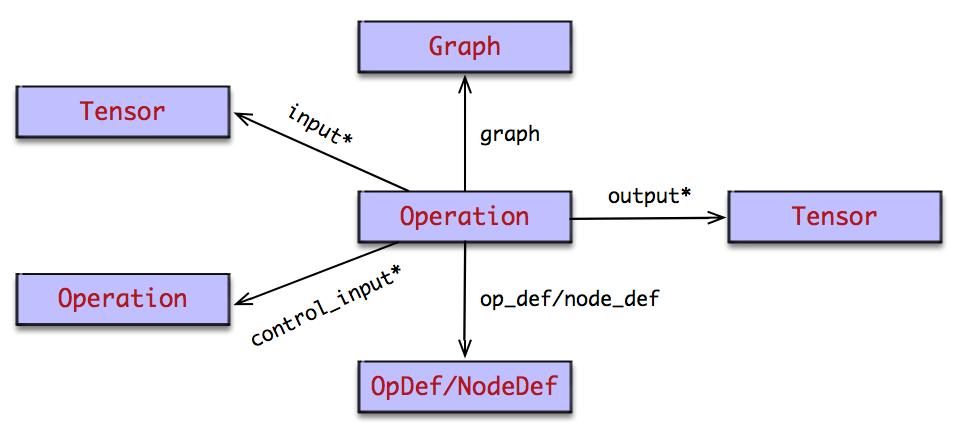
\includegraphics[width=0.9\textwidth]{figures/py-operation.png}
\caption{领域对象:Operation}
 \label{fig:py-operation}
\end{figure}

\subsection{Tensor}

一个\code{Tensor}表示\code{Operation}的某个输出的符号句柄,它并不持\code{Operation}输出的真实数据。可以通过\code{Session.run}计算得到\code{Tensor}所持有的真实数据。

如\refig{py-tensor}所示。\code{Tensor}是两个\code{Operation}数据交换的桥梁,它们之间构造了典型的「生产者-消费者」的关系。

\begin{figure}[!htbp]
\centering
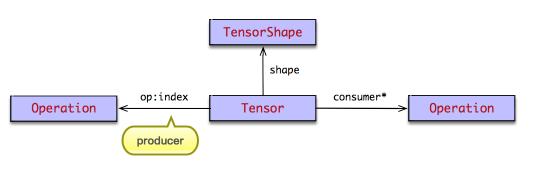
\includegraphics[width=0.9\textwidth]{figures/py-tensor.png}
\caption{领域对象:Tensor}
 \label{fig:py-tensor}
\end{figure}

其中,\code{Tensor}通过\ascii{op}持有扮演生产者角色的\code{Operation},并且使用\code{index}表示该\code{Tensor}在该\code{Operation}输出列表中的索引。也就是说,可以使用\code{op:index}的二元组信息在图中唯一标识一个\code{Tensor}实例。

此外,\code{Tensor}持有\code{Operation}的消费者列表。计算图以\code{Tensor}为边,构建\code{Operation}之间的数据连接,从而实现了整个计算图的数据依赖构建。

\subsubsection{生产者与消费者}

如\refig{py-tensor-producter-consumer}所示。上游\code{Operation}作为生产者,经过某种抽象计算,生产了一个\code{Tensor},并以此作为该上游\code{Operation}的输出之一,并使用\code{index}标识。

该\code{Tensor}被传递给下游\code{Operation},并作为下游\code{Operation}的输入,下游\code{Operation}充当该\code{Tensor}的消费者。

\begin{figure}[!htbp]
\centering
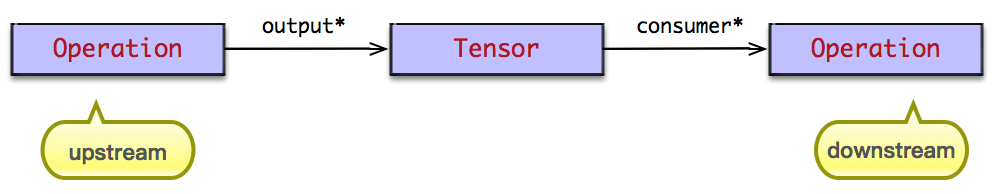
\includegraphics[width=0.9\textwidth]{figures/py-tensor-producter-consumer.png}
\caption{Tensor: 生产者-消费者关系}
 \label{fig:py-tensor-producter-consumer}
\end{figure}

\subsubsection{建立关联}

最后,参看\code{Operation}与\code{Tensor}的部分实现,很容易找两者「生产者-消费者」的关联关系。当\code{Tensor}列表作为输入流入\code{Operation}时,此时建立了下游\code{Operation}与输入的\code{Tensor}列表之间的消费关系。

\begin{leftbar}
\begin{python}
class Operation(object):
  def __init__(self, node_def, graph, inputs=None, output_types=None):
    # \_inputs as consumers
    self._inputs = list(inputs)
    for a in self._inputs:
      a._add_consumer(self)

    # self as producer
    self._output_types = output_types
    self._outputs = [Tensor(self, i, output_type)
                     for i, output_type in enumerate(output_types)]
\end{python}
\end{leftbar}


同样地,\code{Tensor}在构造函数中持有作为上游的的生产者\code{Operation},及其它在该\code{Operation}的\code{outputs}列表中的索引。此外,当调用\code{\_add\_consumer},将该下游\code{Operation}追加至消费者列表之中。

\begin{leftbar}
\begin{python}
class Tensor(_TensorLike):
  def __init__(self, op, value_index, dtype):    
    # Index of the OP's endpoint that produces this tensor.
    self._op = op
    self._value_index = value_index
    
    # List of operations that use this Tensor as input.  
    # We maintain this list to easily navigate a computation graph.
    self._consumers = []

  def _add_consumer(self, consumer):
    if not isinstance(consumer, Operation):
      raise TypeError("Consumer must be an Operation: %s" % consumer)
    self._consumers.append(consumer)
\end{python}
\end{leftbar}

\subsection{Graph}

如\refig{py-graph}所示。一个\code{Graph}对象将包含一系列\code{Operation}对象,表示计算单元的集合;同时,它间接持有一系列\code{Tensor}对象,表示数据单元的集合。

\begin{figure}[!htbp]
\centering
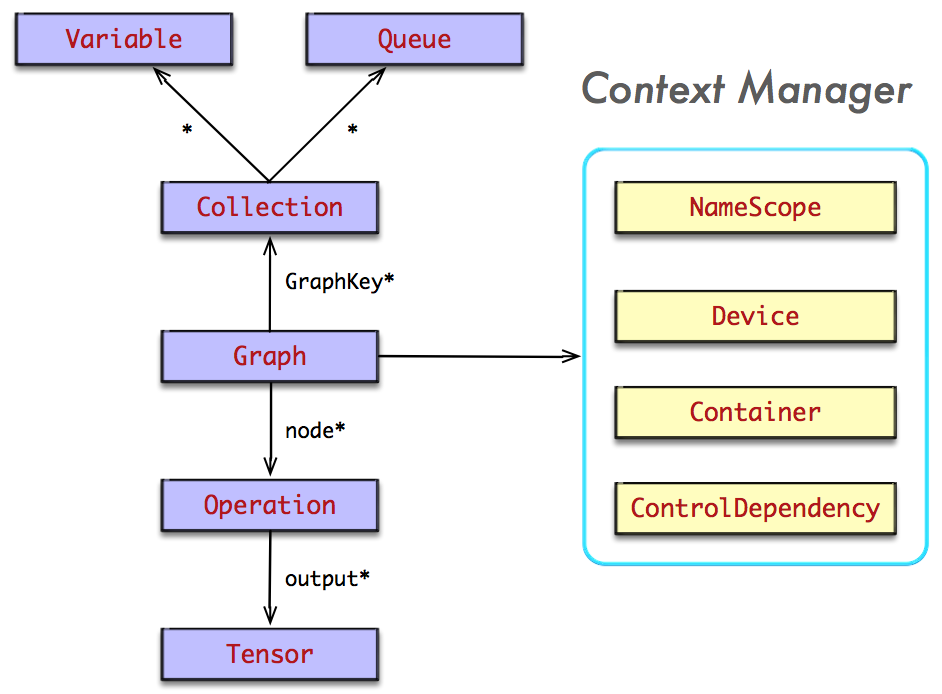
\includegraphics[width=0.9\textwidth]{figures/py-graph.png}
\caption{领域对象:Graph}
 \label{fig:py-graph}
\end{figure}

\subsection{图构造}

在计算图的构造期间,不执行任何\ascii{OP}的计算。简单地说,图的构造过程就是根据\ascii{OP}构造器完成\code{Operation}实例的构造。而在\code{Operation}实例的构造之前,需要实现完成\code{OpDef}与\code{NodeDef}的构造过程。

\subsubsection{OpDef仓库}

\code{OpDef}仓库在系统首次访问时,实现了\code{OpDef}的延迟加载和注册。也就是说,对于某中类型的\code{OpDef}仓库,\code{\_InitOpDefLibrary}模块首次导入时,扫描\code{op\_list\_ascii}表示的所有\ascii{OP},并将其转换为\ascii{Protobuf}格式的\code{OpList}实例,最终将其注册到\code{OpDefLibrary}实例之中。

例如,模块\code{gen\_array\_ops}是构建版本时自动生成的,它主要完成所有\code{array\_ops}类型的\code{OpDef}的定义,并自动注册到\code{OpDefLibrary}的仓库实例中,并提供按名查找\code{OpDef}的服务接口。

\begin{leftbar}
\begin{python}
_op_def_lib = _InitOpDefLibrary()

def _InitOpDefLibrary():
  op_list = _op_def_pb2.OpList()
  _text_format.Merge(_InitOpDefLibrary.op_list_ascii, op_list)   
  op_def_lib = _op_def_library.OpDefLibrary()
  op_def_lib.add_op_list(op_list)
  return op_def_lib

_InitOpDefLibrary.op_list_ascii = """op {
  name: "ZerosLike"
  input_arg {
    name: "x"
    type_attr: "T"
  }
  output_arg {
    name: "y"
    type_attr: "T"
  }
  attr {
    name: "T"
    type: "type"
  }
}
# ignore others
"""
\end{python}
\end{leftbar}

\subsubsection{工厂方法}

如\refig{py-op-factory-and-repo}所示。当\ascii{Client}使用\ascii{OP}构造器创建一个\code{Operation}实例时,将最终调用\code{Graph.create\_op}方法,将该\code{Operation}实例注册到该图实例中。

也就是说,一方面,\code{Graph}充当\code{Operation}的工厂,负责\code{Operation}的创建职责;另一方面,\code{Graph}充当\code{Operation}的仓库,负责\code{Operation}的存储,检索,转换等操作。

这个过程常称为计算图的构造。在计算图的构造期间,并不会触发运行时的\ascii{OP}运算,它仅仅描述计算节点之间的依赖关系,并构建\ascii{DAG}图,对整个计算过程做整体规划。

\begin{figure}[!htbp]
\centering
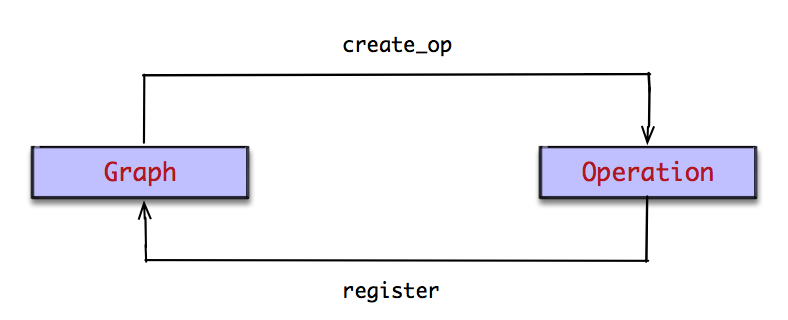
\includegraphics[width=0.9\textwidth]{figures/py-op-factory-and-repo.png}
\caption{Graph: OP工厂 + OP仓库}
 \label{fig:py-op-factory-and-repo}
\end{figure}

\subsubsection{OP构造器}

如\refig{py-op-constructor}所示。在图构造期,\ascii{Client}使用\code{tf.zeros\_like}构造一个名为\code{ZerosLike}的\ascii{OP},该\ascii{OP}拥有一个输入,输出一个全\ascii{0}的\ascii{Tensor};其中,\code{tf.zeros\_like}常称为\ascii{OP}构造器。

然后,\ascii{OP}构造器调用一段自动生成的代码,进而转调\code{OpDefLibrary.apply\_op}方法。

\begin{figure}[!htbp]
\centering
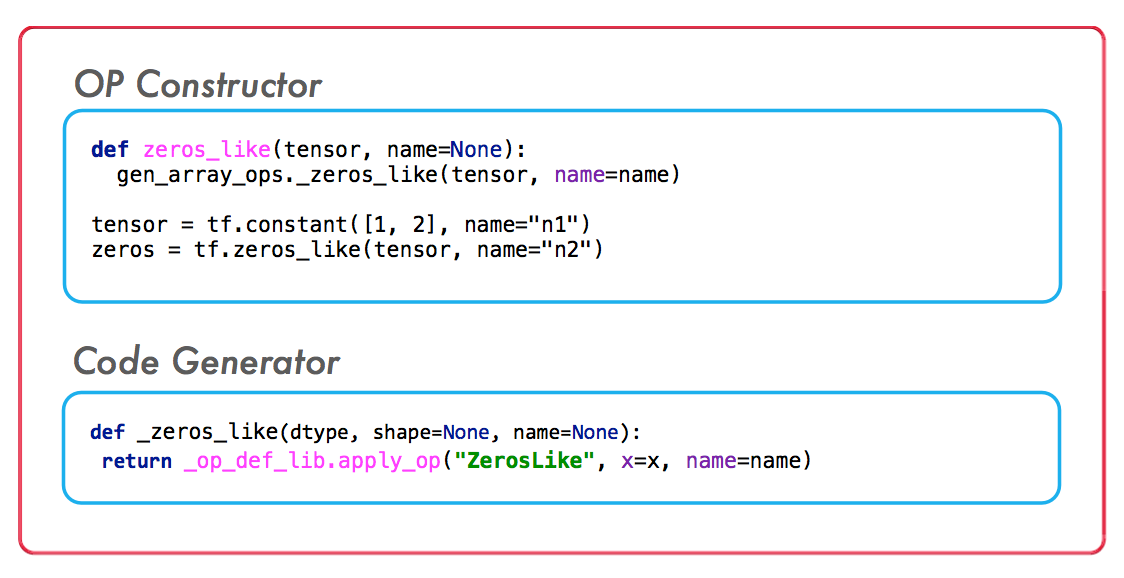
\includegraphics[width=0.9\textwidth]{figures/py-op-constructor.png}
\caption{OP构造器与代码生成器}
 \label{fig:py-op-constructor}
\end{figure}

\subsubsection{构造OpDef与NodeDef}

然后,如\refig{py-graph-create-op}所示。\code{OpDefLibrary}根据\ascii{OP}的名字从\code{OpDefLibrary}中,找到对应\code{OpDef}实例;最终,通过\code{Graph.create\_op}的工厂方法,创建\code{NodeDef}实例,进而创建\code{Operation}实例,将其自身注册到图实例中。

\begin{figure}[!htbp]
\centering
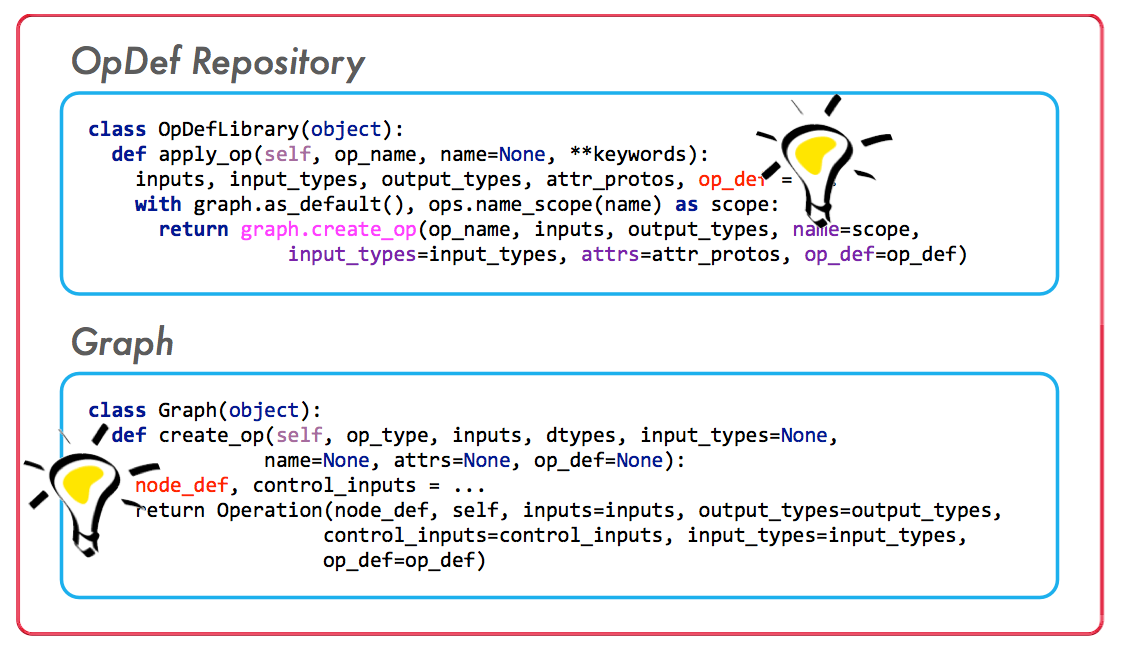
\includegraphics[width=0.9\textwidth]{figures/py-graph-create-op.png}
\caption{创建Operation实例: 创建OpDef, NodeDef实例}
 \label{fig:py-graph-create-op}
\end{figure}

\end{content}

\section{后端C++}

\begin{content}

在\ascii{C++}后端,计算图是\ascii{TensorFlow}领域模型的核心。

\subsection{边}

\code{Edge}持有前驱节点与后驱节点,从而实现了计算图的连接。一个节点可以拥有零条或多条输入边,与可以有零条或多条输出边。一般地,计算图中存在两类边:

\begin{enum}
  \eitem{普通边:用于承载数据(以\code{Tensor}表示),表示节点间“生产者-消费者”的数据依赖关系,常用实线表示;}
  \eitem{控制依赖:不承载数据,用于表示节点间的执行依赖关系,常用虚线表示。} 
\end{enum}

\subsubsection{两个标识}

\ascii{Edge}持有两个重要的索引:

\begin{enum}
  \eitem{\code{src\_output}:表示该边为「前驱节点」的第\code{src\_output}条输出边;}
  \eitem{\code{dst\_input}:表示该边为「后驱节点」的第\code{dst\_input}条输入边。} 
\end{enum}


\begin{figure}[!htbp]
\centering
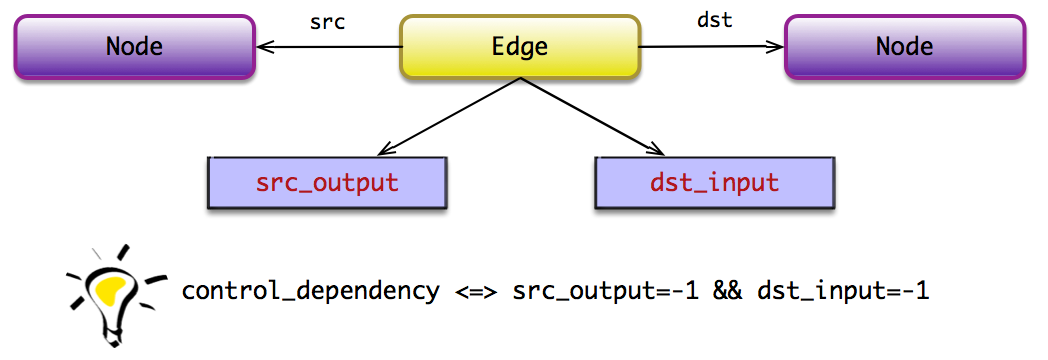
\includegraphics[width=0.9\textwidth]{figures/cc-edge-model.png}
\caption{领域对象:Edge}
 \label{fig:cc-edge-model}
\end{figure}

例如,存在两个前驱节点\code{s1, s2},都存在两条输出边;存在两个后驱节点\code{d1, d2},都存在两条输入边。

\begin{figure}[!htbp]
\centering
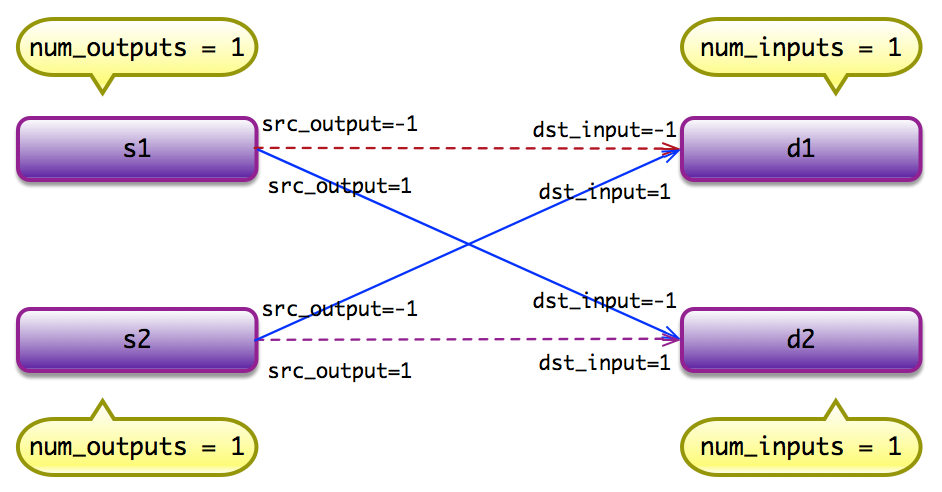
\includegraphics[width=0.9\textwidth]{figures/cc-edge-model-example.png}
\caption{边例子}
 \label{fig:cc-edge-model-example}
\end{figure}

\subsubsection{控制依赖}

对于控制依赖边,其\code{src\_output, dst\_input}都为\code{-1(Graph::kControlSlot)},暗喻控制依赖边不承载任何数据。

\begin{leftbar}
\begin{c++}
bool Edge::IsControlEdge() const {
   // or dst\_input\_ == Graph::kControlSlot;
   return src_output_ == Graph::kControlSlot;
}
\end{c++}
\end{leftbar}

\subsubsection{Tensor标识}

一般地,计算图的「普通边」承载\code{Tensor},并使用\code{TensorId}标识。\code{Tensor}标识由源节点的名字,及其所在边的\code{src\_output}唯一确定。

\begin{leftbar}
\begin{c++}
TensorId ::= node_name:src_output
\end{c++}
\end{leftbar}

缺省地,\code{src\_output}默认为\ascii{0};也就是说,\code{node\_name}与\code{node\_name:0}两者等价。特殊地,当\code{src\_output}等于\ascii{-1}时,表示该边为「控制依赖边」,\code{TensorId}可以标识为\code{\^node\_name},标识该边依赖于\code{node\_name}所在的节点。

\subsection{节点}

\code{Node}(节点)可以拥有零条或多条输入/输出的边,并使用\code{in\_edges, out\_edges}分别表示输入边和输出边的集合。另外,\code{Node}持有\code{NodeDef, OpDef}。其中,\code{NodeDef}包含设备分配信息,及其\ascii{OP}的属性值列表;\code{OpDef}持有\ascii{OP}的元数据,包括\ascii{OP}输入输出类型等信息。

\begin{figure}[!htbp]
\centering
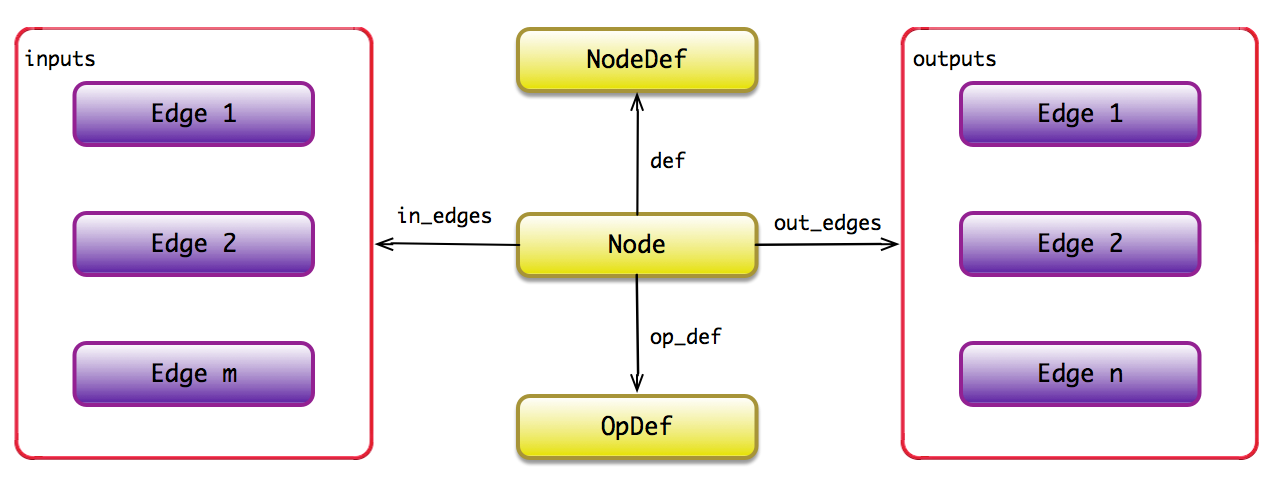
\includegraphics[width=0.9\textwidth]{figures/cc-node-model.png}
\caption{领域对象:Node}
 \label{fig:cc-node-model}
\end{figure}

\subsubsection{输入边}

在输入边的集合中,可以按照索引\code{(dst\_input)}线性查找。当节点输入的边比较多时,可能会成为性能的瓶颈。依次类推,按照索引\code{(src\_output)}查找输出边,算法类同。

\begin{leftbar}
\begin{c++}
Status Node::input_edge(int idx, const Edge** e) const {
  for (auto edge : in_edges()) {
    if (edge->dst_input() == idx) {
      *e = edge;
      return Status::OK();
    }
  }
  return errors::NotFound("not found input edge ", idx);
}
\end{c++}
\end{leftbar}

\subsubsection{前驱节点}

首先通过\code{idx}索引找到输入边,然后通过输入边找到前驱节点。依次类推,按照索引查找后驱节点,算法类同。

\begin{leftbar}
\begin{c++}
Status Node::input_node(int idx, const Node** n) const {
  const Edge* e = nullptr;
  TF_RETURN_IF_ERROR(input_edge(idx, &e));
  *n = e == nullptr ? nullptr : e->src();
  return Status::OK();
}
\end{c++}
\end{leftbar}

\subsection{图}

\code{Graph}(计算图)就是节点与边的集合。计算图是一个\ascii{DAG}图,计算图的执行过程将按照\ascii{DAG}的拓扑排序,依次启动\ascii{OP}的运算。其中,如果存在多个入度为\ascii{0}的节点,\ascii{TensorFlow}运行时可以实现并发,同时执行多个\ascii{OP}的运算,提高执行效率。

\begin{figure}[!htbp]
\centering

\includegraphics[width=0.9\textwidth]{figures/cc-graph-model.png}
\caption{领域模型:图}
 \label{fig:cc-graph-model}
\end{figure}

\subsubsection{空图}

计算图的初始状态,并非是一个空图。实现添加了两个特殊的节点:\code{Source}与\code{Sink}节点,分别表示\ascii{DAG}图的起始节点与终止节点。其中,\code{Source}的\code{id}为\ascii{0},\code{Sink}的\code{id}为\ascii{1};依次论断,普通\ascii{OP}节点的\ascii{id}将大于\ascii{1}。

\code{Source}与\code{Sink}之间,通过连接「控制依赖」的边,保证计算图的执行始于\code{Source}节点,终于\code{Sink}节点。它们之前的控制依赖边,其\code{src\_output, dst\_input}值都为\ascii{-1}。

\begin{figure}[!htbp]
\centering
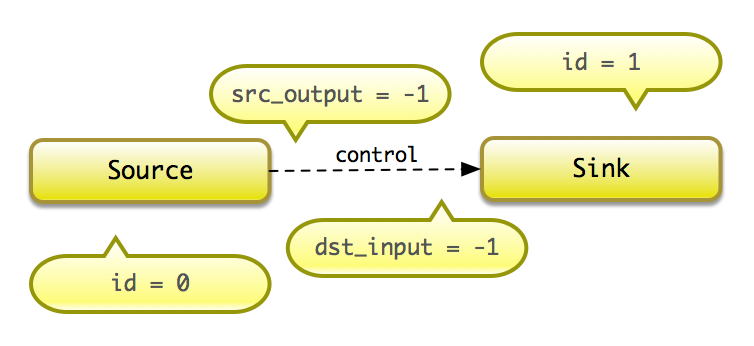
\includegraphics[width=0.9\textwidth]{figures/cc-empty-graph.png}
\caption{空图}
 \label{fig:cc-empty-graph}
\end{figure}

\code{Source}与\code{Sink}是两个内部实现保留的节点,其节点名称以下划线开头,分别使用\code{\_SOURCE}和\code{\_SINK}命名;并且,它们都是\code{NoOp},表示不执行任何计算。

\begin{leftbar}
\begin{c++}
Node* Graph::AddInternalNode(const char* name, int id) {
  NodeDef def;
  def.set_name(name);
  def.set_op("NoOp");

  Status status;
  Node* node = AddNode(def, &status);
  TF_CHECK_OK(status);
  CHECK_EQ(node->id(), id);
  return node;
}

Graph::Graph(const OpRegistryInterface* ops)
    : ops_(ops), arena_(8 << 10 /* 8kB */) {
  auto src  = AddInternalNode("_SOURCE", kSourceId);
  auto sink = AddInternalNode("_SINK",   kSinkId);
  AddControlEdge(src, sink);
}
\end{c++}
\end{leftbar}

习惯上,仅包含\code{Source}与\code{Sink}节点的计算图也常常称为空图。

\subsubsection{非空图}

在前端,用户使用\ascii{OP}构造器,将构造任意复杂度的计算图。对于运行时,实现将用户构造的计算图通过控制依赖的边与\code{Source/Sink}节点连接,保证计算图执行始于\code{Source}节点,终于\code{Sink}节点。

\begin{figure}[!htbp]
\centering
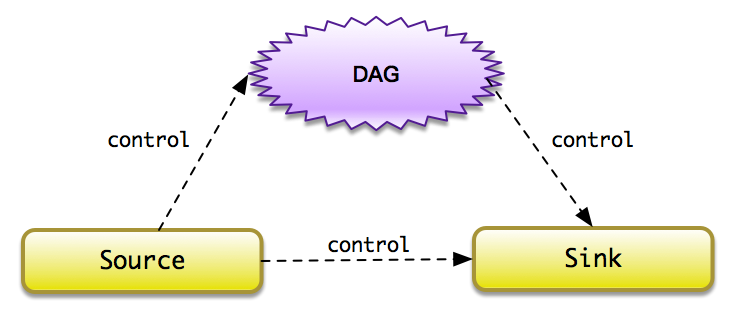
\includegraphics[width=0.9\textwidth]{figures/cc-non-empty-graph.png}
\caption{非空图}
 \label{fig:cc-non-empty-graph}
\end{figure}

\subsubsection{添加边}

计算图的构造过程非常简单,首先通过\code{Graph::AddNode}在图中放置节点,然后再通过\code{Graph::AddEdge}在图中放置边,实现节点之间的连接。

\begin{leftbar}
\begin{c++}
const Edge* Graph::AllocEdge() const {
  Edge* e = nullptr;
  if (free_edges_.empty()) {
    e = new (arena_.Alloc(sizeof(Edge))) Edge;
  } else {
    e = free_edges_.back();
    free_edges_.pop_back();
  }
  e->id_ = edges_.size();
  return e;
}

const Edge* Graph::AddEdge(Node* source, int x, Node* dest, int y) {
  auto e = AllocEdge();
  e->src_ = source;
  e->dst_ = dest;
  e->src_output_ = x;
  e->dst_input_ = y;

  CHECK(source->out_edges_.insert(e).second);
  CHECK(dest->in_edges_.insert(e).second);

  edges_.push_back(e);
  edge_set_.insert(e);
  return e;
}
\end{c++}
\end{leftbar}

\subsubsection{添加控制依赖边}

添加控制依赖边,则可以转发调用\code{Graph::AddEdge}实现;此时,\code{src\_output, dst\_input}都为\ascii{-1}。

\begin{leftbar}
\begin{c++}
const Edge* Graph::AddControlEdge(Node* src, Node* dst) {
  return AddEdge(src, kControlSlot, dst, kControlSlot);
}
\end{c++}
\end{leftbar}

\subsection{OpDef仓库}

同样地,\code{OpDef}仓库在\ascii{C++}系统\code{main}函数启动之前完成\code{OpDef}的加载和注册。它使用\ascii{REGISTER\_OP}宏完成\ascii{OpDef}的注册。

\begin{figure}[!htbp]
\centering
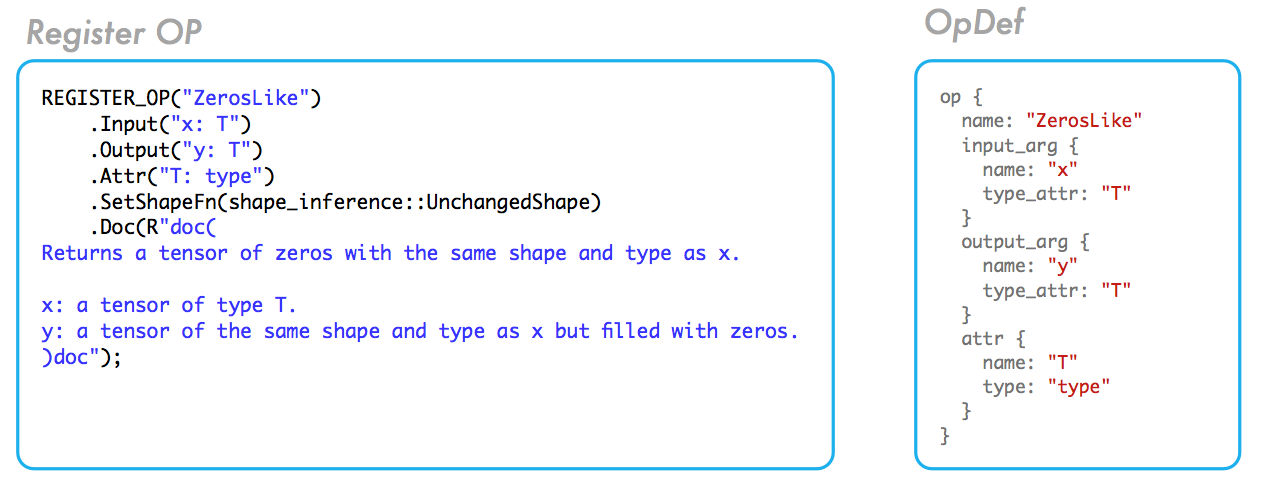
\includegraphics[width=0.9\textwidth]{figures/cc-op-repo.png}
\caption{OpDef注册:使用REGISTER\_OP}
 \label{fig:cc-op-repo}
\end{figure}

\end{content}

\section{图传递}

\begin{content}

\begin{figure}[!htbp]
\centering
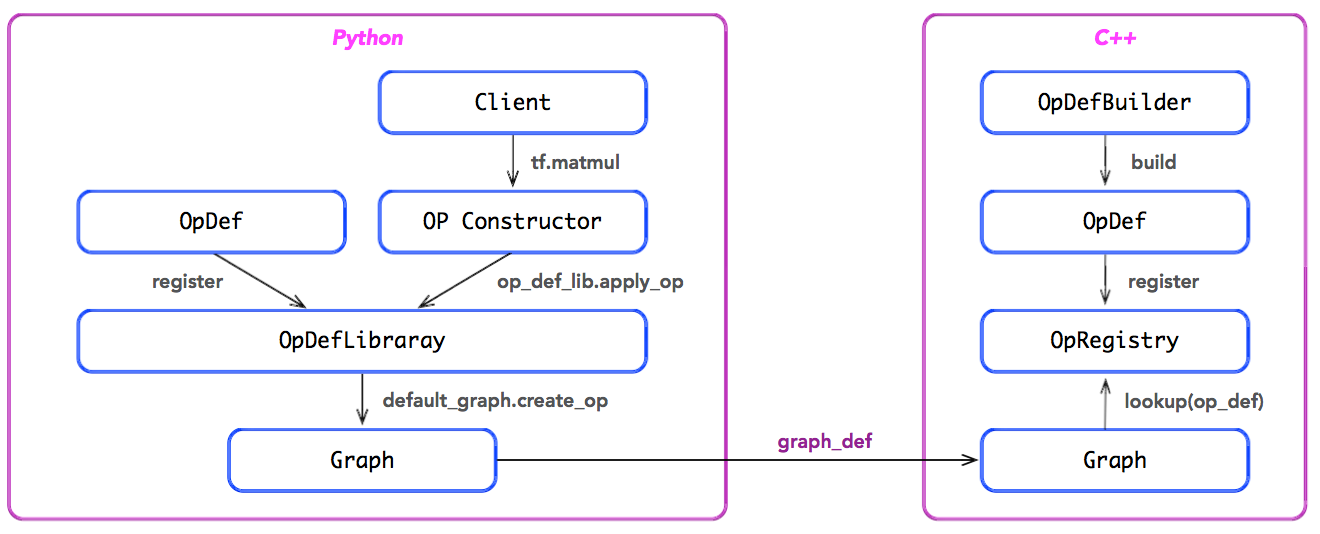
\includegraphics[width=0.9\textwidth]{figures/py-graph-creation.png}
\caption{图的序列化与反序列化}
 \label{fig:py-graph-creation}
\end{figure}

\end{content}


\begin{savequote}[45mm]
\ascii{Any fool can write code that a computer can understand. Good programmers write code that humans can understand.}
\qauthor{\ascii{- Martin Flower}}
\end{savequote}

\chapter{变量} 
\label{ch:variable}

\begin{content}

\ascii{Variable}是一个特殊的\ascii{OP},它拥有状态\ascii{(Stateful)}。从实现技术探究,\ascii{Variable}的\ascii{Kernel}实现直接持有一个\ascii{Tensor}实例,其生命周期与变量一致。相对于普通的\ascii{Tensor}实例,其生命周期仅对本次迭代\ascii{(Step)}有效;而\ascii{Variable}对多个迭代都有效,甚至可以存储到文件系统,或从文件系统中恢复。

\end{content}

\section{实战:线性模型}

\begin{content}

以一个简单的线性模型为例(为了简化问题,此处省略了训练子图)。首先,使用\code{tf.placeholder}定义模型的输入,然后定义了两个全局变量,同时它们都是训练参数,最后定义了一个简单的线性模型。

\begin{leftbar}
\begin{python}
x  = tf.placeholder(tf.float32, [None, 784])
W = tf.Variable(tf.zeros([784,10]), name='W')
b = tf.Variable(tf.zeros([10]), name='b') 
y = tf.matmul(x, W) + b
\end{python}
\end{leftbar}

在使用变量之前,必须对变量进行初始化。按照习惯用法,使用\code{tf.global\_variables}
\code{\_initializer()}将所有全局变量的初始化器汇总,并对其进行初始化。

\begin{leftbar}
\begin{python}
init = tf.global_variables_initializer()

with tf.Session() as sess:
  sess.run(init)
\end{python}
\end{leftbar}

按照既有经验,其计算图大致如\refig{tf-linear-model}所示。

\begin{figure}[!h]
\centering
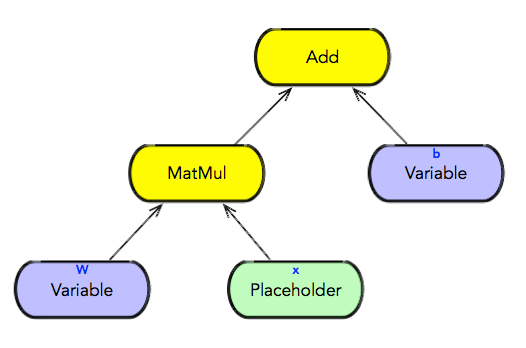
\includegraphics[width=0.6\textwidth]{figures/tf-linear-model.png}
\caption{计算图: 线性加权和}
 \label{fig:tf-linear-model}
\end{figure}

事实上,正如\refig{tf-real-linear-model}所示,实际的计算图要复杂得多,让我们从头说起。

\begin{figure}[!h]
\centering
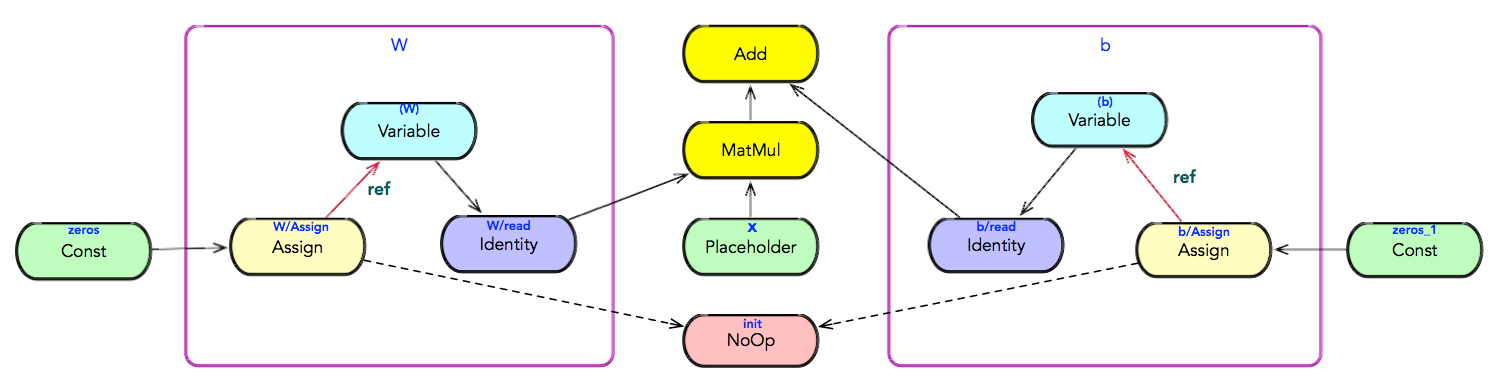
\includegraphics[width=1.0\textwidth]{figures/tf-real-linear-model.png}
\caption{计算图: 线性加权和}
 \label{fig:tf-real-linear-model}
\end{figure}

\end{content}

\section{初始化模型}

\begin{content}

\ascii{Variable}是一个特殊的OP,它拥有状态\ascii{(Stateful)}。如果从实现技术探究,\ascii{Variable}的K\ascii{ernel}实现直接持有一个\ascii{Tensor}实例,其生命周期与\ascii{Variable}一致。相对于普通的\ascii{Tensor}实例,其生命周期仅对本次迭代\ascii{(Step)}有效;而\ascii{Variable}对多个迭代\ascii{(Step)}都有效,甚至可以持久化到文件系统,或从文件系统中恢复。

\subsection{操作变量}

存在几个操作\ascii{Variable}的特殊OP用于修改变量的值,例如\ascii{Assign, AssignAdd}等。\ascii{Variable}所持有的\ascii{Tensor}以引用的方式输入到\ascii{Assign}中,\ascii{Assign}根据初始值\ascii{(Initial Value)}或新值,就地修改\ascii{Tensor}内部的值,最后以引用的方式输出该\ascii{Tensor}。

从设计角度看,\ascii{Variable}可以看做\ascii{Tensor}的包装器,\ascii{Tensor}所支持的所有操作都被\ascii{Variable}重载实现。也就是说,\ascii{Variable}可以出现在\ascii{Tensor}的所有地方。例如,

\begin{leftbar}
\begin{python}
# Create a variable
W = tf.Variable(tf.zeros([784,10]), name='W')

# Use the variable in the graph like any Tensor.
y = tf.matmul(x, W)

# The overloaded operators are available too.
z = tf.sigmoid(w + y)

# Assign a new value to the variable with assign/assign\_add.
w.assign(w + 1.0)
w.assign_add(1.0)
\end{python}
\end{leftbar}

\subsection{初始值}

一般地,在使用变量之前,必须对变量进行初始化。事实上,\ascii{TensorFlow}设计了一个精巧的变量初始化模型。\ascii{Variable}根据初始值\ascii{(Initial Value)}推演\ascii{Variable}的数据类型,并确定\ascii{Tensor}的形状\ascii{(Shape)}。

例如,\code{tf.zeros}称为\ascii{Variable}的初始值,它确定了\ascii{Variable}的类型为\code{int32},且\ascii{Shape}为\code{[784, 10]}。

\begin{leftbar}
\begin{python}
# Create a variable.
W = tf.Variable(tf.zeros([784,10]), name='W')
\end{python}
\end{leftbar}

如下表所示,构造变量初始值的常见\ascii{OP}包括:

\subsection{初始化器}

另外,变量通过初始化器\ascii{(Initializer)}在初始化期间,将初始化值赋予\ascii{Variable}内部所持有\ascii{Tensor},完成\ascii{Variable}的就地修改。

在变量使用之前,必须保证变量被初始化器已初始化。事实上,变量初始化过程,即运行变量的初始化器。

证如上例\code{W}的定义,可以如下完成\code{W}的初始化。此处,\code{W.initializer}实际上为\ascii{Assign}的\ascii{OP},这是\ascii{Variable}默认的初始化器。

\begin{leftbar}
\begin{python}
# Run the variable initializer.
with tf.Session() as sess:
  sess.run(W.initializer)
\end{python}
\end{leftbar}

一旦完成\ascii{Variable}的初始化,其类型与值得以确定。随后可以使用\ascii{Assign}族的\ascii{OP}(例如\ascii{Assign, AssignAdd}等)修改\ascii{Variable}的值。

需要注意的是,在\ascii{TensorBoard}中展示\ascii{Assign}的输入,其边使用特殊的\ascii{ref}标识。数据流向与之刚好相反,否则计算图必然出现环,显然违反了\ascii{DAG}(有向无环图)的基本需求。

\subsection{快照}

如果要读取变量的值,则通过\ascii{Identity}恒等变化,直接输出变量所持有的\ascii{Tensor}。\ascii{Identity}去除了\ascii{Variable}的引用标识,同时也避免了内存拷贝。

\ascii{Identity}操作\ascii{Variable}常称为一个快照\ascii{(Snapshot)},表示\ascii{Variable}当前的值。

事实上,通过\ascii{Identity}将\ascii{Variable}转变为普通的\ascii{Tensor},使得它能够兼容所有\ascii{Tensor}的操作。


\subsection{变量子图}

例如,变量\ascii{W}的定义如下。

\begin{leftbar}
\begin{python}
W = tf.Variable(tf.zeros([784,10]), name='W')
\end{python}
\end{leftbar}

\code{tf.zeros([784,10])}常称为初始值,它通过初始化器\ascii{Assign},将\code{W}内部持有的\ascii{Tensor}以引用的形式就地修改为该初始值;同时,\ascii{Identity}去除了\ascii{Variable}的引用标识,实现了\ascii{Variable}的读取。

\begin{figure}[!h]
\centering
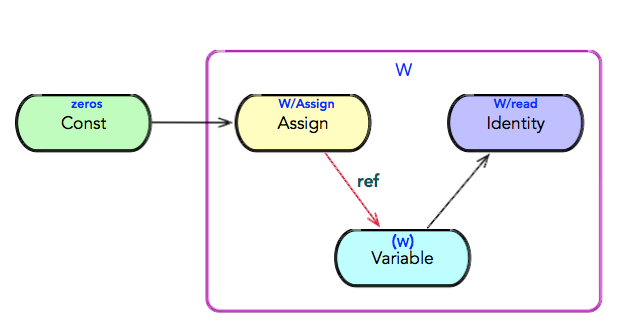
\includegraphics[width=0.8\textwidth]{figures/variable-initialization-model.png}
\caption{变量子图}
 \label{fig:variable-initialization-model}
\end{figure}


\subsection{初始化过程}

更为常见的是,通过调用\code{tf.global\_variables\_initializer()}将所有变量的初始化器进行汇总,然后启动\ascii{Session}运行该\ascii{OP}。

\begin{leftbar}
\begin{python}
init = tf.global_variables_initializer()
\end{python}
\end{leftbar}

事实上,搜集所有全局变量的初始化器的\ascii{OP}是一个\ascii{NoOp},即不存在输入,也不存在输出。所有变量的初始化器通过控制依赖边与该\ascii{NoOp}相连,保证所有的全局变量被初始化。

\begin{figure}[!h]
\centering
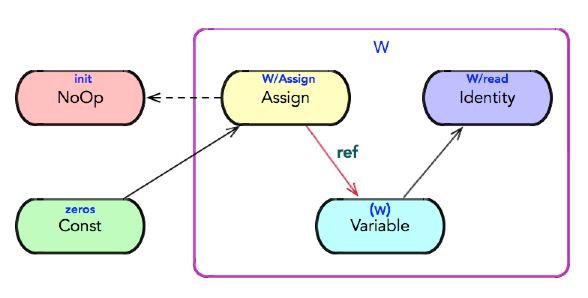
\includegraphics[width=0.8\textwidth]{figures/variable-initialization-no-op.png}
\caption{初始化OP}
 \label{fig:variable-initialization-no-op}
\end{figure}

\subsection{同位关系}

同位关系是一种特殊的设备约束关系。显而易见,\ascii{Assign, Identity}这两个\ascii{OP}与\ascii{Variable}关系极其紧密,分别实现了变量的修改与读取。因此,它们必须与\ascii{Variable}在同一个设备上执行;这样的关系,常称为同位关系\ascii{(Colocation)}。

可以在\ascii{Assign/Identity}节点上指定\code{\_class}属性值:\code{[s: "loc:@W"]},它表示这两个\ascii{OP}与\code{W}放在同一个设备上运行。

例如,以\code{W/read}节点为例,该节点增加了\code{\_class}属性,指示与\code{W}的同位关系。

\begin{leftbar}
\begin{python}
node {
  name: "W/read"
  op: "Identity"
  input: "W"
  attr {
    key: "T"
    value {
      type: DT_FLOAT
    }
  }
  attr {
    key: "_class"
    value {
      list {
        s: "loc:@W"
      }
    }
  }
}
\end{python}
\end{leftbar}

\subsection{初始化依赖}

如果一个变量初始化需要依赖于另外一个变量的初始值,则需要特殊地处理。例如,变量\code{V}的初始值依赖于\code{W}的初始值,可以通过\code{W.initialized\_value()}指定。

\begin{leftbar}
\begin{python}
W = tf.Variable(tf.zeros([784,10]), name='W')
V = tf.Variable(W.initialized_value(), name='V')
\end{python}
\end{leftbar}

事实上,两者通过\ascii{Identity}衔接,并显式地添加了依赖控制边,保证\code{W}在\code{V}之前初始化。此处,存在两个\ascii{Identity}的\ascii{OP},但职责不一样,它们分别完成初始化依赖和变量读取。


\begin{figure}[!h]
\centering
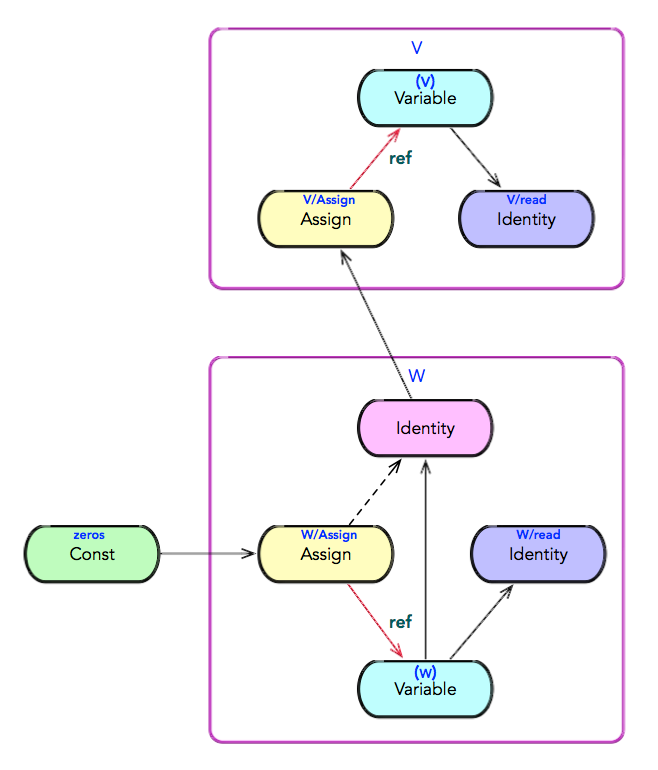
\includegraphics[width=0.8\textwidth]{figures/variable-initialization-dependency-1.png}
\caption{初始化依赖}
 \label{fig:variable-initialization-dependency-1}
\end{figure}

同样地,可以通过调用\code{tf.global\_variables\_initializer()}将变量的所有初始化器进行汇总,然后启动\ascii{Session}完成所有变量的初始化。

\begin{leftbar}
\begin{python}
init = tf.global_variables_initializer()
\end{python}
\end{leftbar}

按照依赖关系,因为增加了\code{W/Assign}与\code{Identity}之间的控制依赖边,从而巧妙地实现了\code{W}在\code{V}之前完成初始化,并通过\code{W}当前的初始化值,最终完成\code{V}的初始化。

\begin{figure}[!h]
\centering
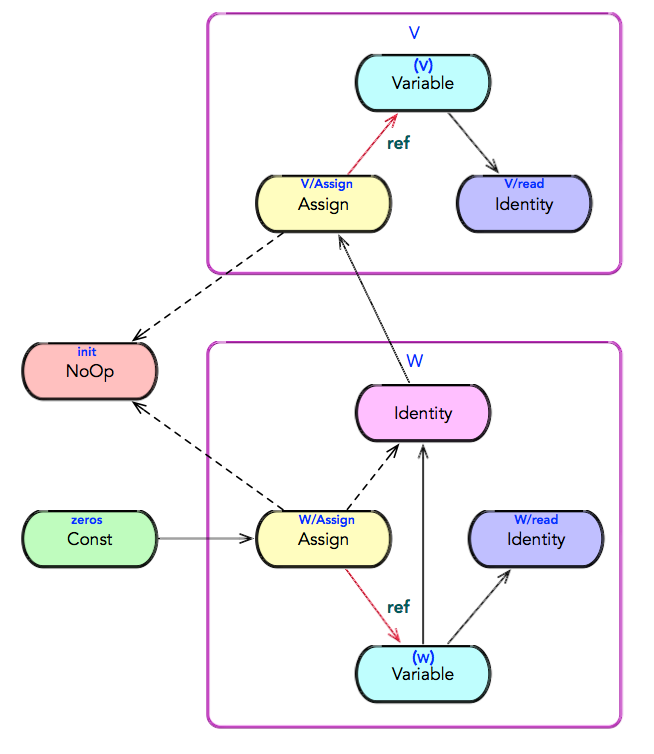
\includegraphics[width=0.8\textwidth]{figures/variable-initialization-dependency-2.png}
\caption{初始化OP}
 \label{fig:variable-initialization-dependency-2}
\end{figure}

\subsection{初始化器列表}

可以使用\code{variables\_initializer}构建变量列表的初始化器列表。其中,\code{group}将构造一个仅控制依赖于\code{\_initialier\_list()}的\ascii{NoOP}。

\begin{leftbar}
\begin{python}
def variables_initializer(var_list, name="init"):
  def _initialier_list():
    return *[v.initializer for v in var_list]
  return control_flow_ops.group(_initialier_list(), name=name)
\end{python}
\end{leftbar}

例如,全局变量列表的初始化器列表可以如下构造。

\begin{leftbar}
\begin{python}
def global_variables_initializer():
  return variables_initializer(global_variables())
\end{python}
\end{leftbar}

\end{content}

\section{变量分组}

\begin{content}

默认地,\ascii{Variable}被划分在全局变量和训练变量的集合中。正如上例,\code{W, V}自动划分至全局变量和训练变量的集合中。

\subsection{全局变量}

可以通过\code{tf.global\_variables()}方便地检索全局变量的集合。在分布式环境中,全局变量能在不同的进程间实现参数共享。

\begin{leftbar}
\begin{python}
def global_variables():
  return ops.get_collection(ops.GraphKeys.GLOBAL_VARIABLES)
\end{python}
\end{leftbar}

\subsection{本地变量}

可以通过\code{tf.local\_variables()}方便地检索本地变量的集合。

\begin{leftbar}
\begin{python}
def local_variables():
  return ops.get_collection(ops.GraphKeys.LOCAL_VARIABLES)
\end{python}
\end{leftbar}

可以使用\code{local\_variable}的语法糖,构建一个本地变量。

\begin{leftbar}
\begin{python}
def local_variable(initial_value, validate_shape=True, name=None):
  return variables.Variable(
      initial_value, trainable=False,
      collections=[ops.GraphKeys.LOCAL_VARIABLES],
      validate_shape=validate_shape, name=name)
\end{python}
\end{leftbar}

本地变量表示进程内的共享变量,它通常不需要做断点恢复\ascii{(Checkpoint)},仅用于临时的计数器的用途。例如,在分布式环境中,使用本地变量记录该进程已读数据的\ascii{Epoch}数目。

\subsection{训练变量}

可以通过\code{tf.trainable\_variables()}检索训练变量的集合。在机器学习中,训练变量表示模型参数。

\begin{leftbar}
\begin{python}
def trainable_variables():
  return ops.get_collection(ops.GraphKeys.TRAINABLE_VARIABLES)
\end{python}
\end{leftbar}

\subsection{global\_step}

\code{global\_step}是一个特殊的\ascii{Variable},它不是训练变量,但它是一个全局变量。在分布式环境中,\code{global\_step}常用于追踪已运行\ascii{step}的次数,并在不同进程间实现数据的同步。

创建一个\code{global\_step}可以使用如下函数:

\begin{leftbar}
\begin{python}
def create_global_step(graph=None):
  graph = ops.get_default_graph() if graph is None else graph
  with graph.as_default() as g, g.name_scope(None):
    collections = [GLOBAL_VARIABLES, GLOBAL_STEP]
    return variable(
        GLOBAL_STEP,
        shape=[],
        dtype=dtypes.int64,
        initializer=init_ops.zeros_initializer(),
        trainable=False,
        collections=collections)
\end{python}
\end{leftbar}

\end{content}

\section{源码分析:构造变量}

\begin{content}

为了简化代码实现,此处对\ascii{Variable}做了简单的重构。

\begin{leftbar}
\begin{python}
class Variable(object):
  def __init__(self, initial_value=None, trainable=True,
    collections=None, name=None, dtype=None):
    with ops.name_scope(name, "Variable", [initial_value]) as name:
      self._cons_initial_value(initial_value, dtype)
      self._cons_variable(name)
      self._cons_initializer()
      self._cons_snapshot()
    self._cons_collections(trainable, collections)
\end{python}
\end{leftbar}

构造\ascii{Variable}实例,基本包括如下几个步骤:

\subsection{构造初始值}

\begin{leftbar}
\begin{python}
  def _cons_initial_value(self, initial_value, dtype):
    self._initial_value = ops.convert_to_tensor(
        initial_value, name="initial_value", dtype=dtype)
\end{python}
\end{leftbar}

\subsection{构造变量OP}

\ascii{Variable}根据初始值的类型和大小完成自动推演。

\begin{leftbar}
\begin{python}
  def _cons_variable(self, name):
    self._variable = state_ops.variable_op_v2(
      self._initial_value.get_shape(),
      self._initial_value.dtype.base_dtype,
      name=name)
\end{python}
\end{leftbar}

\subsection{构造初始化器}

\ascii{Variable}的初始化器本质上是一个\ascii{Assign},它持有\ascii{Variable}的引用,并使用初始值就地修改变量本身。

\begin{leftbar}
\begin{python}
  def _cons_initializer(self):
    self._initializer_op = state_ops.assign(
      self._variable,
      self._initial_value).op
\end{python}
\end{leftbar}

\subsection{构造快照}

\ascii{Variable}的快照本质上是一个\ascii{Identity},表示\ascii{Variable}的当前值。

\begin{leftbar}
\begin{python}
  def _cons_snapshot(self):
    with ops.colocate_with(self._variable.op):
      self._snapshot = array_ops.identity(
        self._variable, name="read")
\end{python}
\end{leftbar}

\subsection{变量分组}

默认地,\ascii{Variable}被划分在全局变量的集合中;如果\code{trainable}为真,则表示该变量为训练参数,并将其划分到训练变量的集合中。

\begin{leftbar}
\begin{python}
  def _cons_collections(self, trainable, collections)
    if collections is None:
      collections = [GLOBAL_VARIABLES]
    if trainable and TRAINABLE_VARIABLES not in collections:
      collections = list(collections) + [TRAINABLE_VARIABLES]
    ops.add_to_collections(collections, self)
\end{python}
\end{leftbar}

\end{content}
\begin{savequote}[45mm]
\ascii{Any fool can write code that a computer can understand. Good programmers write code that humans can understand.}
\qauthor{\ascii{- Martin Flower}}
\end{savequote}

\chapter{设备} 
\label{ch:device}

\begin{content}

\end{content}

\section{设备规范}

\begin{content}

设备规范\ascii{(Device Specification)}用于描述\ascii{OP}存储或计算设备的具体位置。

\subsection{形式化}

一个设备规范可以形式化地描述为:

\begin{leftbar}
\begin{python}
DEVICE_SPEC ::= COLOCATED_NODE | PARTIAL_SPEC
COLOCATED_NODE ::= "@" NODE_NAME
PARTIAL_SPEC ::= ("/" CONSTRAINT) *
CONSTRAINT ::= ("job:" JOB_NAME)
             | ("replica:" [1-9][0-9]*)
             | ("task:" [1-9][0-9]*)
             | ( ("gpu" | "cpu") ":" ([1-9][0-9]* | "*") )
\end{python}
\end{leftbar}

\subsubsection{完整指定}

如下例所示,完整地描述某个\ascii{OP}被放置在\ascii{PS}作业,\ascii{0}号备份,\ascii{0}号任务,\ascii{GPU 0}号设备。

\begin{leftbar}
\begin{python}
/job:ps/replica:0/task:0/device:GPU:0
\end{python}
\end{leftbar}

\subsubsection{部分指定}

设备规范也可以部分指定,甚至为空。例如,下例仅描述了\code{GPU0}号设备。

\begin{leftbar}
\begin{python}
/device:GPU:0
\end{python}
\end{leftbar}

特殊地,当设备规范为空时,则表示对\ascii{OP}未实施设备约束,运行时自动选择设备放置\ascii{OP}。

\subsubsection{同位}

使用\code{COLOCATED\_NODE}指示该\ascii{OP}与指定的节点被同时放置在相同的设备上。例如,该节点与\code{other/node}放置在相同的设备上。

\begin{leftbar}
\begin{python}
@other/node  # colocate with "other/node"
\end{python}
\end{leftbar}

\subsubsection{DeviceSpec}

一个设备规范可以使用字符串,或者\code{DeviceSpec}表示。其中,\code{DeviceSpec}是一个值对象,使用如下\ascii{5}个标识确定设备规范。

\begin{enum}
  \eitem{作业名称}
  \eitem{备份索引}
  \eitem{任务索引}
  \eitem{设备类型}
  \eitem{设备索引}
\end{enum}

例如,使用\code{DeviceSpec}构造的设备规范。

\begin{leftbar}
\begin{python}
# '/job:ps/replica:0/task:0/device:CPU:0'
DeviceSpec(job="ps", replica=0, task=0, device_type="CPU", device_index=0)
\end{python}
\end{leftbar}

\subsection{上下文管理器}

常常使用上下文管理器\code{device(device\_spec)}指定\ascii{OP}设备规范,在该上下文的作用域内构造的\code{OP}在运行时将被放置在指定设备上运行。

\begin{leftbar}
\begin{python}
with g.device('/gpu:0'):
  # All OPs constructed here will be placed on GPU 0.
\end{python}
\end{leftbar}

其中,\code{device}是\code{Graph}的一个方法,它设计了一个栈式结构的上下文管理器,实现设备规范的闭包、合并、覆盖等特性。

\subsubsection{合并}

可以对两个不同范围的设备规范进行合并。

\begin{leftbar}
\begin{python}
with device("/job:ps"):
  # All OPs constructed here will be placed on PS.
  with device("/task:0/device:GPU:0"):
    # All OPs constructed here will be placed on
    # /job:ps/task:0/device:GPU:0
\end{python}
\end{leftbar}

\subsubsection{覆盖}

在合并两个相同范围的设备规范时,内部指定的设备规范具有高优先级,实现设备规范的覆盖。

\begin{leftbar}
\begin{python}
with device("/device:CPU:0"):
  # All OPs constructed here will be placed on CPU 0.
  with device("/job:ps/device:GPU:0"):
    # All OPs constructed here will be placed on
    # /job:ps/device:GPU:0
\end{python}
\end{leftbar}

\subsubsection{重置}

特殊地,当内部的设备规范置位为\code{None}时,将忽略外部所有设备规范的定义。

\begin{leftbar}
\begin{python}
with device("/device:GPU:0"):
  # All OPs constructed here will be placed on CPU 0.
  with device(None):
    # /device:GPU:0 will be ignored.
\end{python}
\end{leftbar}

\subsubsection{设备规范函数}

当指定设备规范时,常常使用字符串,或\code{DeviceSpec}进行描述。也可以使用更加灵活的\emph{设备规范函数},它提供了一种更加灵活的扩展方式指定设备规范。设备规范函数是一个回调函数,入参为\code{Operation},生成一个字符串格式的设备规范。

\begin{leftbar}
\begin{python}
def matmul_on_gpu(n):
 if n.type == "MatMul":
   return "/gpu:0"
 else:
   return "/cpu:0"

with g.device(matmul_on_gpu):
  # All OPs of type "MatMul" constructed in this context
  # will be placed on GPU 0; all other OPs will be placed
  # on CPU 0.
\end{python}
\end{leftbar}

\subsubsection{实现}

\code{Graph.device(spec)}实现了一个栈式结构的上下文管理器,它可以接受字符串格式的设备规范,或者\emph{设备规范函数}。事实上,当给\code{device}函数传递字符串,或者\code{DeviceSpec}时,首先会对该字符串,或\code{DeviceSpec}做一个简单的适配,统一转换为设备规范函数。

\begin{leftbar}
\begin{python}
class Graph(object):
  def device(self, device_name_or_func):
    def to_device_func():
      if (device_name_or_func is not None
          and not callable(device_name_or_func)):
        return pydev.merge_device(device_name_or_func)
      else:
        return device_name_or_func

    try:
      self._device_function_stack.append(to_device_func())
      yield
    finally:
      self._device_function_stack.pop()
\end{python}
\end{leftbar}

当用户使用\code{device}时,未显式地指定图实例,则隐式地使用全局唯一的默认图实例。也就是说,\code{tf.device(spec)}函数事实上是对\code{get\_default\_graph().device(spec)}的一个简单包装。

\begin{leftbar}
\begin{python}
# tensorflow/python/framework/ops.py
def device(device_name_or_function):
  return get_default_graph().device(device_name_or_function)
\end{python}
\end{leftbar}

\subsubsection{应用}

在\code{Graph.device}实现中,\code{pydev.merge\_device}生成一个设备规范函数。该设备函数以输入的\code{spec}创建新的副本,通过调用\code{copy\_spec.merge\_from(current\_device)},合并既有的\code{node\_def.device}设备规范,并且\code{node\_def.device}具有更高的优先级。实现较为隐晦,为什么\code{node\_def.device}具有较高优先级呢?这取决于\code{\_apply\_device\_functions}实现覆盖、合并、重置的需求。

\begin{leftbar}
\begin{python}
def merge_device(spec):
  # replace string to DeviceSpec
  if not isinstance(spec, DeviceSpec):
    spec = DeviceSpec.from_string(spec or "")

  # returns a device function that merges devices specifications
  def _device_function(node_def):
    current_device = DeviceSpec.from_string(node_def.device or "")
    copy_spec = copy.copy(spec)

    # IMPORTANT: `node\_def.device` takes precedence.
    copy_spec.merge_from(current_device)      
    return copy_spec
  return _device_function
\end{python}
\end{leftbar}

当\code{Graph.create\_op}时,将调用\code{\_apply\_device\_functions}设置\code{NodeDef}的设备规范。它将对\code{\_device\_function\_stack}依次实施出栈操作,并调用相应的设备规范函数,并将结果直接设置为\code{NodeDef}的设备规范。如此,内嵌指定的\code{device}具有较高优先级,实现了合并、覆盖、重置外围指定的\code{device}。

\begin{leftbar}
\begin{python}
class Graph(object):
  def _apply_device_functions(self, op):
    for device_function in reversed(self._device_function_stack):
      if device_function is None:
        break
      # IMPORTANT: `node\_def.device` takes precedence.  
      op._set_device(device_function(op)) 
\end{python}
\end{leftbar}

\end{content}

\begin{savequote}[45mm]
\ascii{Any fool can write code that a computer can understand. Good programmers write code that humans can understand.}
\qauthor{\ascii{- Martin Flower}}
\end{savequote}

\chapter{会话} 
\label{ch:session}

\begin{content}

客户端以\code{Session}为桥梁,与后台计算引擎建立连接,并启动计算图的执行过程。其中,通过调用\code{Session.run}将触发\ascii{TensorFlow}的一次计算\ascii{(Step)}。

事实上,\code{Session}建立了执行计算图的闭包环境,它封装了\ascii{OP}计算,及其\ascii{Tensor}求值的计算环境。

\end{content}

\section{资源管理}

\begin{content}

在\code{Session}的生命周期中,将根据计算图的计算需求,按需分配系统资源,包括变量,队列,读取器等。

\subsection{关闭会话}

当计算完成后,需要确保\code{Session}被安全地关闭,以便安全释放所管理的系统资源。

\begin{leftbar}
\begin{python}
sess = tf.Session()
sess.run(targets)
sess.close()
\end{python}
\end{leftbar}

\subsection{上下文管理器}

一般地,常常使用上下文管理器创建\code{Session},使得\code{Session}在计算完成后,能够自动关闭,确保资源安全性地被释放。

\begin{leftbar}
\begin{python}
with tf.Session() as sess:
  sess.run(targets)
\end{python}
\end{leftbar}

\subsection{图实例}

一个\code{Session}实例,只能运行一个图实例;但是,一个图实例,可以运行在多个\code{Session}实例中。如果尝试在同一个\code{Session}运行另外一个图实例,必须先关闭\code{Session}(不必销毁),再启动新图的计算过程。

虽然一个\code{Session}实例,只能运行一个图实例。但是,可以\code{Session}是一个线程安全的类,可以并发地执行该图实例上的不同子图。例如,一个典型的机器学习训练模型中,可以使用同一个\code{Session}实例,并发地运行输入子图,训练子图,及其\ascii{Checkpoint}子图。

\subsubsection{引用计数器}

为了提高效率,避免计算图频繁地创建与销毁,存在一种实现上的优化技术。在图实例中维护一个\code{Session}的引用计数器,当且仅当\code{Session}的数目为零时,才真正地销毁图实例。

\begin{figure}[!htbp]
\centering
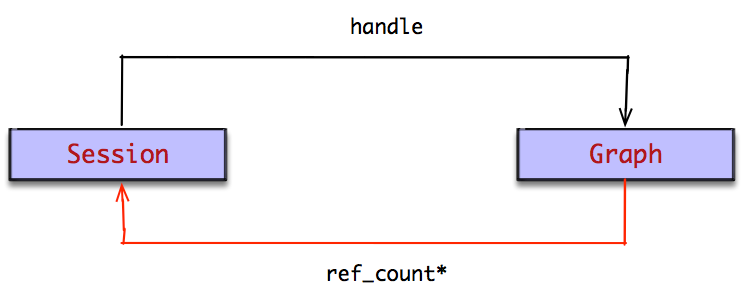
\includegraphics[width=0.7\textwidth]{figures/tf-graph-session-relation.png}
\caption{优化技术:会话实例的引用计数器}
 \label{fig:tf-graph-session-relation}
\end{figure}

\subsubsection{数据结构}

此处,摘取\code{TF\_Graph}部分关于\code{Session}引用计数器技术的关键字段;其中,\code{TF\_Graph}结构体定义于\ascii{C API}的头文件。

\begin{leftbar}
\begin{c++}
struct TF_Graph {
  TF_Graph();

  tensorflow::mutex mu;
  tensorflow::Graph graph GUARDED_BY(mu);

  // TF\_Graph may only and must be deleted when
  // num\_sessions == 0 and delete\_requested == true

  // num\_sessions incremented by TF\_NewSession, 
  // and decremented by TF\_DeleteSession.
  int num_sessions GUARDED_BY(mu);
  bool delete_requested GUARDED_BY(mu);
};
\end{c++}
\end{leftbar}

同理,\code{TF\_Session}持有一个二元组:\code{<tensorflow::Sesssion, TF\_Graph>},它们之间是一对一的关系。其中,\code{tensorflow::Sesssion}是\ascii{C++}客户端侧的会话实例。

\begin{leftbar}
\begin{c++}
struct TF_Session {
  TF_Session(tensorflow::Session* s, TF_Graph* g)
      : session(s), graph(g), last_num_graph_nodes(0) {}
  tensorflow::Session* session;
  TF_Graph* graph;
  tensorflow::mutex mu;
  int last_num_graph_nodes;
};
\end{c++}
\end{leftbar}

\subsubsection{创建会话}

\begin{leftbar}
\begin{c++}
TF_Session* TF_NewSession(TF_Graph* graph, const TF_SessionOptions* opt,
                          TF_Status* status) {
  Session* session;
  status->status = NewSession(opt->options, &session);
  if (status->status.ok()) {
    if (graph != nullptr) {
      mutex_lock l(graph->mu);
      graph->num_sessions += 1;
    }
    return new TF_Session(session, graph);
  } else {
    DCHECK_EQ(nullptr, session);
    return nullptr;
  }
}
\end{c++}
\end{leftbar}

\subsubsection{销毁会话}

\begin{leftbar}
\begin{c++}
void TF_DeleteSession(TF_Session* s, TF_Status* status) {
  status->status = Status::OK();
  TF_Graph* const graph = s->graph;
  if (graph != nullptr) {
    graph->mu.lock();
    graph->num_sessions -= 1;
    const bool del = graph->delete_requested && graph->num_sessions == 0;
    graph->mu.unlock();
    if (del) delete graph;
  }
  delete s->session;
  delete s;
}
\end{c++}
\end{leftbar}

\section{默认会话}

\begin{content}

通过调用\ascii{Session.as\_default()},将该\code{Session}置为默认\code{Session},同时它返回了一个上下文管理器。在默认\code{Session}的上文中,可以直接实施\ascii{OP}的运算,或者\ascii{Tensor}的求值。

\begin{leftbar}
\begin{python}
hello = tf.constant('hello, world')

sess = tf.Session()  
with sess.as_default():
  print(hello.eval())
sess.close()
\end{python}
\end{leftbar}

但是,\code{Session.as\_default()}并不会自动关闭\code{Session},需要用户显式地调用\code{Session.close}方法。

\subsection{张量求值}

如上例代码,\code{hello.eval()}等价于\code{tf.get\_default\_session().run(hello)}。其中,\code{Tensor.eval}如下代码实现。

\begin{leftbar}
\begin{python}
class Tensor(_TensorLike):
  def eval(self, feed_dict=None, session=None):
    if session is None:
      session = get_default_session()
    return session.run(tensors, feed_dict)
\end{python}
\end{leftbar}

\subsection{OP运算}

同理,当用户未显式提供\code{Session},\code{Operation.run}将自动获取默认的\code{Session}实例,并按照当前\ascii{OP}的依赖关系,以某个特定的拓扑排序执行该计算子图。

\begin{leftbar}
\begin{python}
class Operation(object):
  def run(self, feed_dict=None, session=None):
    if session is None:
      session = tf.get_default_session()
    session.run(self, feed_dict)
\end{python}
\end{leftbar}

\subsection{线程相关}

默认会话仅仅对当前线程有效,以便在当前线程追踪Session的调用栈。如果在新的线程中使用默认会话,需要在线程函数中通过调用\code{as\_default}将\code{Session}置为默认会话。

事实上,在\ascii{TensorFlow}运行时维护了一个\code{Session}的本地线程栈,实现默认\code{Session}的自动管理。

\begin{leftbar}
\begin{python}
_default_session_stack = _DefaultStack()

def get_default_session(session):
  return _default_session_stack.get_default(session)
\end{python}
\end{leftbar}

其中,\code{\_DefaultStack}表示栈的数据结构。

\begin{leftbar}
\begin{python}
class _DefaultStack(threading.local):
  def __init__(self):
    super(_DefaultStack, self).__init__()
    self.stack = []

  def get_default(self):
    return self.stack[-1] if len(self.stack) >= 1 else None

  @contextlib.contextmanager
  def get_controller(self, default):
    try:
      self.stack.append(default)
      yield default
    finally:
      self.stack.remove(default)
\end{python}
\end{leftbar}

\end{content}

\section{会话类型}

\begin{content}

一般地,存在两种基本的会话类型:\code{Session}与\code{InteractiveSession}。后者常常用于交互式环境,它在构造期间将其自身置为默认,简化默认会话的管理过程。

此外,两者在运行时的配置也存在差异。例如,\code{InteractiveSession}将\code{GPUOptions.allow\_growth}置为\code{True},避免在实验环境中独占整个GPU的存储资源。

\begin{figure}[!htbp]
\centering
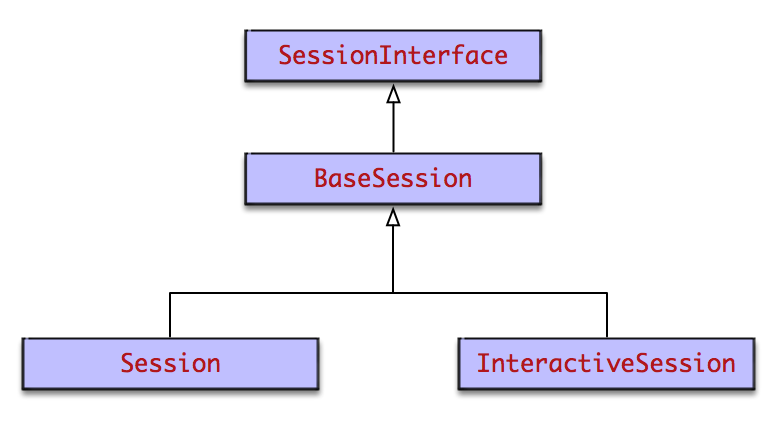
\includegraphics[width=0.7\textwidth]{figures/py-session-hierarchy.png}
\caption{Session:类层次结构}
 \label{fig:py-session-hierarchy}
\end{figure}

\subsection{Session}

\code{Session}继承\code{BaseSession},并增加了默认图与默认会话的上下文管理器的功能,保证系统资源的安全释放。

一般地,使用\code{with}进入会话的上下文管理器,并自动切换默认图与默认会话的上下文;退出\code{with}语句时,将自动关闭默认图与默认会话的上下文,并自动关闭会话。

\begin{leftbar}
\begin{python}
class Session(BaseSession):
  def __init__(self, target='', graph=None, config=None):
    super(Session, self).__init__(target, graph, config=config)
    self._default_graph_context_manager = None
    self._default_session_context_manager = None

  def __enter__(self):
    self._default_graph_context_manager = self.graph.as_default()
    self._default_session_context_manager = self.as_default()

    self._default_graph_context_manager.__enter__()
    return self._default_session_context_manager.__enter__()

  def __exit__(self, exec_type, exec_value, exec_tb):
    self._default_session_context_manager.__exit__(
        exec_type, exec_value, exec_tb)
    self._default_graph_context_manager.__exit__(
        exec_type, exec_value, exec_tb)

    self._default_session_context_manager = None
    self._default_graph_context_manager = None

    self.close()
\end{python}
\end{leftbar}

\subsection{InteractiveSession}

与\code{Session}不同,\code{InteractiveSession}在构造期间将其自身置为默认,并实现默认图与默认会话的自动切换。与此相反,\code{Session}必须借助于\code{with}语句才能完成该功能。在交互式环境中,\code{InteractiveSession}简化了用户管理默认图和默认会话的过程。

同理,\code{InteractiveSession}在计算完成后需要显式地关闭,以便安全地释放其所占用的系统资源。

\begin{leftbar}
\begin{python}
class InteractiveSession(BaseSession):
  def __init__(self, target='', graph=None, config=None):
    super(InteractiveSession, self).__init__(target, graph, config)

    self._default_session_context_manager = self.as_default()
    self._default_session_context_manager.__enter__()

    self._default_graph_context_manager = graph.as_default()
    self._default_graph_context_manager.__enter__()

  def close(self):
    super(InteractiveSession, self).close()
    self._default_graph.__exit__(None, None, None)
    self._default_session.__exit__(None, None, None)
\end{python}
\end{leftbar}

\subsection{BaseSession}

\code{BaseSession}是两者的基类,它主要实现会话的创建,关闭,执行,销毁等管理生命周期的操作;它与后台计算引擎相连接,实现前后端计算的交互。

\subsubsection{创建会话}

通过调用\ascii{C API}的接口,\code{self.\_session}直接持有后台计算引擎的会话句柄,后期执行计算图,关闭会话等操作都以此句柄为标识。

\begin{leftbar}
\begin{python}
class BaseSession(SessionInterface):
  def __init__(self, target='', graph=None, config=None):
    # ignore implements...
    with errors.raise_exception_on_not_ok_status() as status:
      self._session = 
        tf_session.TF_NewDeprecatedSession(opts, status)
\end{python}
\end{leftbar}

\subsubsection{执行计算图}

通过调用\code{run}接口,实现计算图的一次计算。它首先通过\code{tf\_session.TF\_ExtendGraph}将图注册给后台计算引擎,然后再通过调用\code{tf\_session.TF\_Run}启动计算图的执行。

\begin{leftbar}
\begin{python}
class BaseSession(SessionInterface):
  def run(self, 
    fetches, feed_dict=None, options=None, run_metadata=None):
    self._extend_graph()
    with errors.raise_exception_on_not_ok_status() as status:
      return tf_session.TF_Run(session, 
        options, feed_dict, fetch_list, 
        target_list, status, run_metadata)
  
  def _extend_graph(self):
    with errors.raise_exception_on_not_ok_status() as status:
      tf_session.TF_ExtendGraph(self._session,
        graph_def.SerializeToString(), status)  
\end{python}
\end{leftbar}

\subsubsection{关闭会话}

\begin{leftbar}
\begin{python}
class BaseSession(SessionInterface):
  def close(self):
    with errors.raise_exception_on_not_ok_status() as status:
      tf_session.TF_CloseDeprecatedSession(self._session, status)
\end{python}
\end{leftbar}

\subsubsection{销毁会话}

\begin{leftbar}
\begin{python}
class BaseSession(SessionInterface):
  def __del__(self):
    try:
      status = tf_session.TF_NewStatus()
      tf_session.TF_DeleteDeprecatedSession(self._session, status)
    finally:
      tf_session.TF_DeleteStatus(status)
\end{python}
\end{leftbar}

\begin{content}
\begin{savequote}[45mm]
\ascii{Any fool can write code that a computer can understand. Good programmers write code that humans can understand.}
\qauthor{\ascii{- Martin Flower}}
\end{savequote}

\chapter{Saver} 
\label{ch:saver}

\section{Saver}

\begin{content}

在长期的训练任务过程中,为了实现任务的高可用性,\tf{}会周期性地执行断点检查(\ascii{Checkpoint})。

\code{Saver}是实现断点检查功能的基础设施,它会将所有的训练参数持久化在文件系统中;当需要恢复训练时,可以载从文件系统中恢复计算图,及其训练参数的值。也就是说,\code{Saver}承担如下两个方面的职责:

\begin{enum}
  \eitem{\code{save}: 将训练参数的当前值持久化到断点文件中;}
  \eitem{\code{restore}: 从断点文件中恢复训练参数的值。} 
\end{enum}

\subsection{使用方法}

例如,存在一个简单的计算图,包含两个训练参数。首先,执行初始化后,将其结果持久化到文件系统中。

\begin{leftbar}
\begin{python}
# construct graph
v1 = tf.Variable([0], name='v1')
v2 = tf.Variable([0], name='v2')

# run graph
with tf.Session() as sess:
  sess.run(tf.global_variables_initializer())
  saver = tf.train.Saver()
  saver.save(sess, 'ckp')
\end{python}
\end{leftbar}

随后,可以根据断点文件存储的位置恢复模型。

\begin{leftbar}
\begin{python}
with tf.Session() as sess:
  saver = tf.import_meta_graph('ckp.meta')
  saver.restore(sess, 'ckp')
\end{python}
\end{leftbar}

\subsection{文件功能}

当执行\code{Saver.save}操作之后,在文件系统中生成如下文件:

\begin{leftbar}
\begin{python}
├── checkpoint
├── ckp.data-00000-of-00001
├── ckp.index
├── ckp.meta
\end{python}
\end{leftbar}

\subsubsection{索引文件}

索引(\ascii{index})文件保存了一个不可变表(\code{tensorflow::table::Table})的数据;其中,关键字为\ascii{Tensor}的名称,其值描述该\ascii{Tensor}的元数据信息,包括该\ascii{Tensor}存储在哪个数据(\ascii{data})文件中,及其在该数据文件中的偏移,及其校验和等信息。

\subsubsection{数据文件}

数据(\ascii{data})文件记录了所有变量\ascii{(Variable)}的值。当\code{restore}某个变量时,首先从索引文件中找到相应变量在哪个数据文件,然后根据索引直接获取变量的值,从而实现变量数据的恢复。

\subsubsection{元文件}

元文件(\ascii{meta})中保存了\code{MetaGraphDef}的持久化数据,它包括\code{GraphDef, SaverDef}等元数据。

将描述计算图的元数据与存储变量值的数据文件相分离,实现了静态的图结构与动态的数据表示的分离。因此,在恢复\ascii{(Restore)}时,先调用\code{tf.import\_meta\_graph}先将\code{GraphDef}恢复出来,然后再恢复\code{SaverDef},从而恢复了描述静态图结构的\code{Graph}对象,及其用于恢复变量值的\code{Saver}对象,最后使用\code{Saver.restore}恢复所有变量的值。

这也是在上例中,在调用\code{Saver.restore}之前,得先调用\code{tf.import\_meta\_graph}的真正原因;否则,缺失计算图的实例,就无法谈及恢复数据到图实例中了。

\subsubsection{状态文件}

\ascii{Checkpoint}文件会记录最近一次的断点文件(\ascii{Checkpoint File})的前缀,根据前缀可以找对对应的索引和数据文件。当调用\code{tf.train.latest\_checkpoint},可以快速找到最近一次的断点文件。


此外,\ascii{Checkpoint}文件也记录了所有的断点文件列表,并且文件列表按照由旧至新的时间依次排序。当训练任务时间周期非常长,断点检查将持续进行,必将导致磁盘空间被耗尽。为了避免这个问题,存在两种基本的方法:

\begin{enum}
  \eitem{\code{max\_to\_keep}: 配置最近有效文件的最大数目,当新的断点文件生成时,且文件数目超过\code{max\_to\_keep},则删除最旧的断点文件;其中,\code{max\_to\_keep}默认值为\ascii{5};}
  \eitem{\code{keep\_checkpoint\_every\_n\_hours}: 在训练过程中每\code{n}小时做一次断点检查,保证只有一个断点文件;其中,该选项默认是关闭的。} 
\end{enum}

由于\ascii{Checkpoint}文件也记录了断点文件列表,并且文件列表按照由旧至新的时间依次排序。根据上述策略删除陈旧的断点文件将变得极其简单有效。

\subsection{模型}

\subsubsection{持久化模型}

为了实现持久化的功能,\code{Saver}在构造时在计算图中插入\code{SaveV2},及其关联的\ascii{OP}。其中,\code{file\_name}为一个\ascii{Const}的\ascii{OP},指定断点文件的名称;\code{tensor\_names}也是一个\ascii{Const}的\ascii{OP},用于指定训练参数的\ascii{Tensor}名称列表。

\begin{figure}[!htbp]
\centering
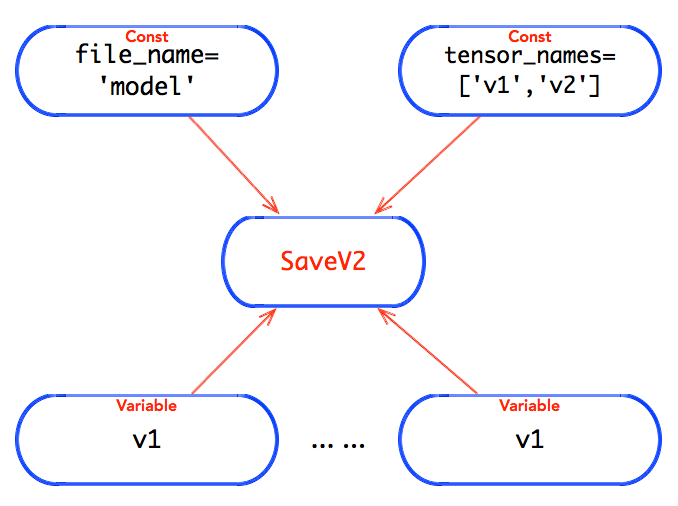
\includegraphics[width=0.5\textwidth]{figures/py-saver-save-model.png}
\caption{Saver:持久化模型}
 \label{fig:py-saver-save-model}
\end{figure}

\subsubsection{恢复模型}

同样地,为了实现恢复功能,\code{Saver}在构造期,为每个训练参数,插入了一个\code{RestoreV2},及其关联的\ascii{OP}。其中,包括从断点文件中恢复参数默认值的初始化器\ascii{(Initializer)},其本质是一个\code{Assign}的\ascii{OP}。 

另外,\code{file\_name}为一个\ascii{Const}的\ascii{OP},指定断点文件的名称;\code{tensor\_names}也是一个\ascii{Const}的\ascii{OP},用于指定训练参数的\ascii{Tensor}名称列表,其长度为\ascii{1}。

\begin{figure}[!htbp]
\centering
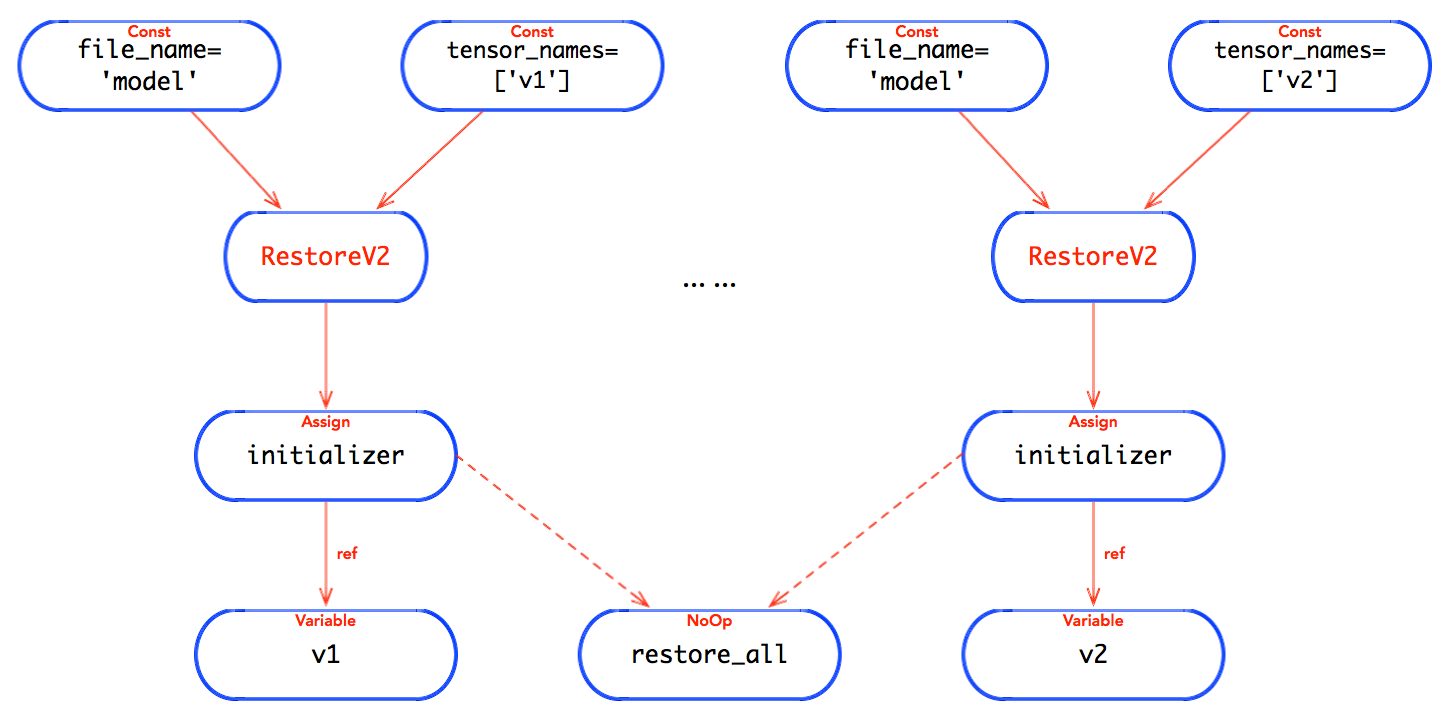
\includegraphics[width=0.9\textwidth]{figures/py-saver-restore-model.png}
\caption{Saver:恢复模型}
 \label{fig:py-saver-restore-model}
\end{figure}

\end{content}

\begin{savequote}[45mm]
\ascii{Any fool can write code that a computer can understand. Good programmers write code that humans can understand.}
\qauthor{\ascii{- Martin Flower}}
\end{savequote}

\chapter{MonitoredSession} 
\label{ch:monitored-session}

\begin{content}

训练一个简单的模型,可以通过运行\code{train\_op}数次直至模型收敛,最终将训练参数实施\ascii{Checkpoint},持久化训练模型。对于小规模的学习模型,这个过程至多需要花费数小时的时间。

但是,对于大规模的学习模型,需要花费数天时间;而且可能需要使用多份复本\ascii{(replica)},此时需要更加健壮的训练过程支持模型的训练。因此,需要解决三个基本问题:

\begin{enum}
  \eitem{当训练过程异常关闭,或程序崩溃,能够合理地处理异常;}
  \eitem{当异常关闭,或程序崩溃之后,能够恢复训练过程;} 
  \eitem{能够通过\ascii{TensorBoard}监控整个训练过程。}   
\end{enum}

当训练被异常关闭或程序崩溃之后,为了能够恢复训练过程,必须周期性实施\ascii{Checkpoint}。当训练过程重启后,可以通过寻找最近一次的\ascii{Checkpoint}文件,恢复训练过程。

为了能够使用\ascii{TensorBoard}监控训练过程,可以通过周期性运行一些\ascii{Summary}的\ascii{OP},并将结果追加到事件文件中。\ascii{TensorBoard}能够监控和解析事件文件的数据,可视化整个训练过程,包括展示计算图的结构。

\end{content}

\section{引入MonitoredSession}

\begin{content}

\code{tf.train.MonitoredSession},它可以定制化\code{Hook},用于监听整个\code{Session}的生命周期;内置\code{Coordinator}对象,用于协调所有运行中的线程同时停止,并监听,上报和处理异常;当发生\code{AbortedError}或\code{UnavailableError}异常时,可以重启\code{Session}。

\subsection{使用方法}

一般地,首先使用\code{ChiefSessionCreator}创建\code{Session}实例,并且注册三个最基本的\code{tf.train.SessionRunHook}:

\begin{enum}
  \eitem{\code{CheckpointSaverHook}:周期性地\ascii{Checkpoint};}
  \eitem{\code{SummarySaverHook}:周期性地运行\ascii{Summary};} 
  \eitem{\code{StepCounterHook}:周期性地统计每秒运行的\ascii{Step}数目。}   
\end{enum}

为了能够安全处理异常,并且能够关闭\code{MonitoredSession},常常使用\code{with}的上下文管理器。

\begin{leftbar}
\begin{python}
session_creator = tf.train.ChiefSessionCreator(
  checkpoint_dir=checkpoint_dir,
  master=master,
  config=config)

hooks = [
  tf.train.CheckpointSaverHook(
    checkpoint_dir=checkpoint_dir,
    save_secs=save_checkpoint_secs),
  tf.train.SummarySaverHook(
    save_secs=save_summaries_secs,
    output_dir=checkpoint_dir),
  tf.train.StepCounterHook(
    output_dir=checkpoint_dir, 
    every_n_steps=log_step_count_steps)
]

with tf.train.MonitoredSession(
  session_creator=session_creator,
  hooks=hooks) as sess:
  if not sess.should_stop():
    sess.run(train_op)
\end{python}
\end{leftbar}

\subsection{使用工厂}

使用\code{MonitoredTrainingSession}的工厂方法,可以简化\code{MonitoredSession}的创建过程。

\begin{figure}[!htbp]
\centering
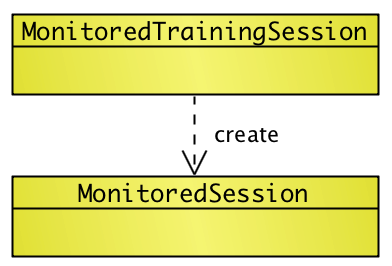
\includegraphics[width=0.4\textwidth]{figures/py-train-monitored-training-session.png}
\caption{MonitoredTrainingSession:工厂方法}
 \label{fig:py-train-monitored-training-session}
\end{figure}

\begin{leftbar}
\begin{python}
with MonitoredTrainingSession(
  master=master,
  is_chief=is_chief,
  checkpoint_dir=checkpoint_dir
  config=config) as sess:
  if not sess.should_stop():
    sess.run(train_op)
\end{python}
\end{leftbar}

\subsection{装饰器}

为了得到复合功能的\code{MonitoredSession},可以将完成子功能的\code{WrappedSession}进行组合拼装。

\begin{enum}
  \eitem{\code{RecoverableSession}:当发生\code{AbortedError}或\code{UnavailableError}异常时,可以恢复和重建\code{Session};}
  \eitem{\code{CoordinatedSession}:内置\code{Coordinator}对象,用于协调所有运行中的线程同时停止,并监听,上报和处理异常;} 
  \eitem{\code{HookedSession}:可以定制化\code{Hook},用于监听整个\code{Session}的生命周期。}   
\end{enum}

\begin{figure}[!htbp]
\centering
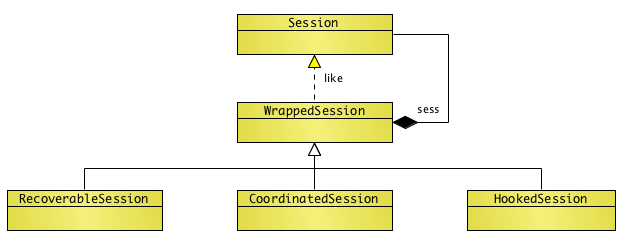
\includegraphics[width=0.9\textwidth]{figures/py-train-monitored-session-decorator.png}
\caption{MonitoredSession:装饰器}
 \label{fig:py-train-monitored-session-decorator}
\end{figure}

最终,可以组合三者的特性,构建得到\code{MonitoredSession}(伪代码实现,详情请查阅\code{MonitoredSession}的具体实现)。

\begin{leftbar}
\begin{python}
MonitoredSession(
  RecoverableSession(
    CoordinatedSession(
      HookedSession(
        tf.Session(target, config)))))
\end{python}
\end{leftbar}

\end{content}

\section{生命周期}

\begin{content}

\code{MonitoredSession}具有\code{Session}的生命周期特征(但并非\ascii{IS-A}关系,而是\ascii{Like-A}关系,这是一种典型的按照鸭子编程的风格)。

在生命周期过程中,插入了\code{SessionRunHook}的回调钩子,用于监听\code{MonitoredSession}的生命周期过程。

\subsection{初始化}

在初始化阶段,\code{MonitoredSession}主要完成如下过程:

\begin{enum}
  \eitem{运行所有回调钩子的\code{begin}方法;}
  \eitem{通过调用\code{scaffold.finalize()}冻结计算图;} 
  \eitem{创建会话:使用\code{SessionCreator}多态创建\code{Session}}   
  \eitem{运行所有回调钩子的\code{after\_create\_session}方法}
\end{enum}

其中,使用\code{SessionCreator}多态创建\ascii{Session}的过程,存在两种类型。

\begin{enum}
  \eitem{\code{ChiefSessionCreator}:调用\code{SessionManager.prepare\_session},通过从最近的\ascii{Checkpoing}恢复模型,或运行\code{init\_op},完成模型的初始化;然后,启动所有\code{QueueRunner}实例;}
  \eitem{\code{WorkerSessionCreator}:调用\code{SessionManager.wait\_for\_session},等待\code{Chief}完成模型的初始化。} 
\end{enum}

\begin{figure}[!htbp]
\centering
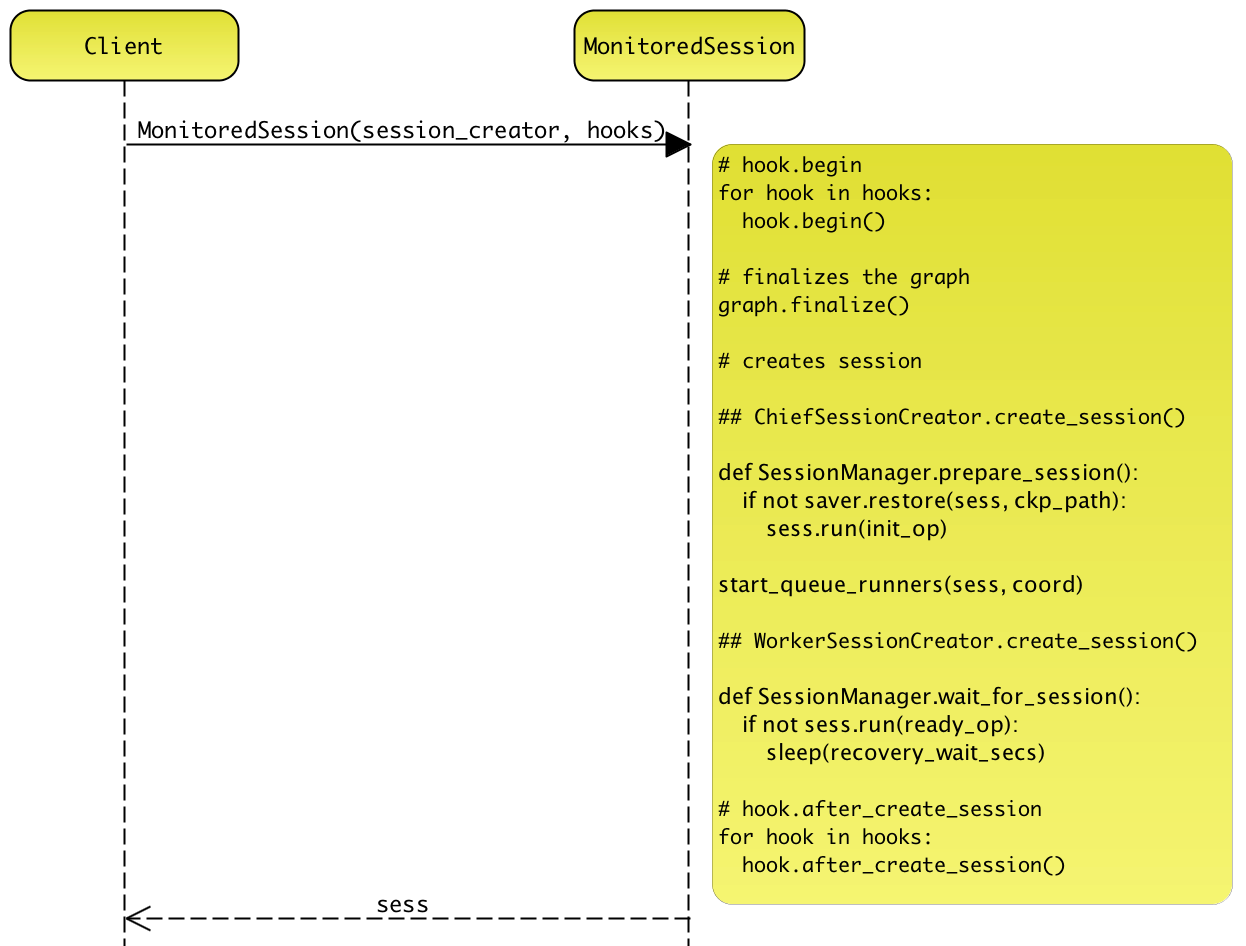
\includegraphics[width=0.9\textwidth]{figures/py-train-monitored-session-initialization.png}
\caption{MonitoredSession:初始化}
 \label{fig:py-train-monitored-session-initialization}
\end{figure}

\subsection{执行}

在执行阶段,在运行\code{Session.run}前后分别回调钩子的\code{before\_run}和\code{after\_run}方法。如果在运行过程发生了\code{AbortedError}或\code{UnavailableError}异常,则重启会话服务。

\begin{figure}[!htbp]
\centering
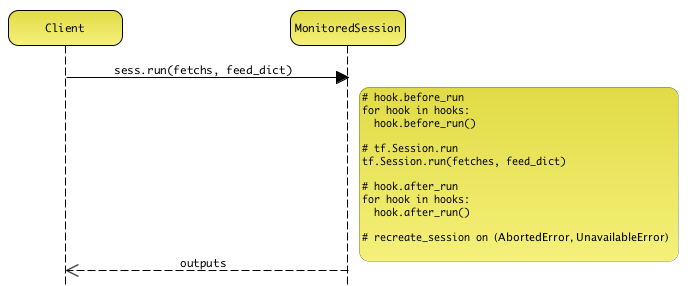
\includegraphics[width=0.9\textwidth]{figures/py-train-monitored-session-execution.png}
\caption{MonitoredSession:执行}
 \label{fig:py-train-monitored-session-execution}
\end{figure}

\subsection{关闭}

当训练过程结束后,通过调用\code{close}方法,关闭\code{MonitoredSession},释放系统的计算资源。

此时,将回调钩子的\code{end}方法,并且会通过调用\code{Coordinator.request\_stop}方法,停止所有\code{QueueRunner}实例。最终,听过调用\code{tf.Session.close}方法,释放系统的资源。

另外,如果发生\code{OutOfRangeError}异常,\code{MonitoredSession}认为训练过程正常终止,并忽略该异常。

\begin{figure}[!htbp]
\centering
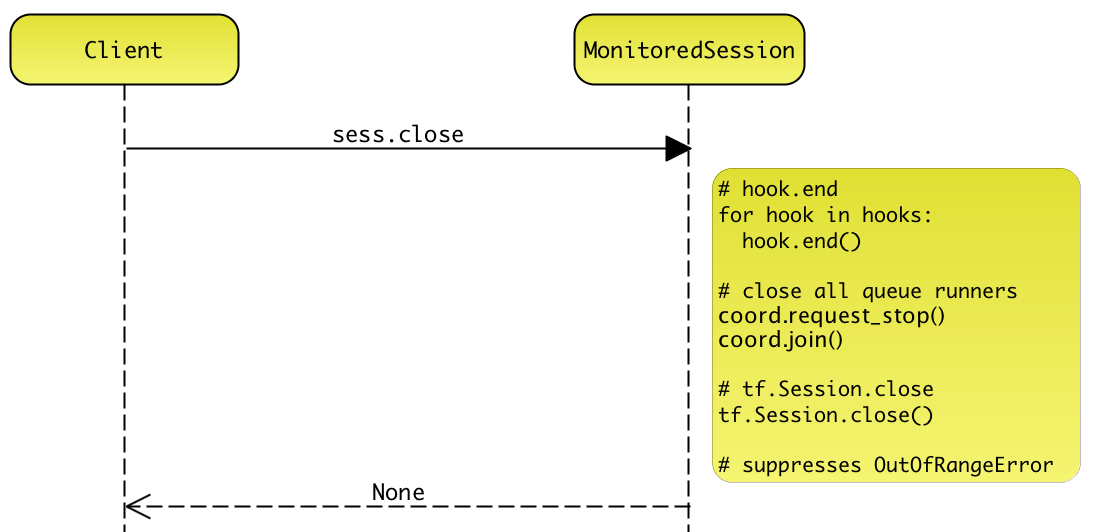
\includegraphics[width=0.9\textwidth]{figures/py-train-monitored-session-close.png}
\caption{MonitoredSession:关闭}
 \label{fig:py-train-monitored-session-close}
\end{figure}

\end{content}

\section{模型初始化}

\begin{content}

\code{MonitoredSession}在初始化时,使用\code{SessionCreator}完成会话的创建和模型的初始化。

一般地,在分布式环境下,存在两种类型的\ascii{Worker}:

\begin{enum}
  \eitem{\ascii{Chief}: 负责模型的初始化;}
  \eitem{\ascii{Non-Chief}: 等待\ascii{Chief}完成模型的初始化。} 
\end{enum}

两者之间,通过一个简单的协调协议共同完成模型的初始化。

\subsection{协调协议}

对于\ascii{Chief},它会尝试从\ascii{Checkpoint}文件中恢复模型;如果没有成功,则会通过执行\code{init\_op}全新地初始化模型;其初始化算法,可以形式化描述为:

\begin{leftbar}
\begin{python}
def prepare_session(master, init_op, saver, ckp_dir):
  if is_chief():
    sess = tf.Session(master)
    sess.run(init_op) if not saver.restore(sess, ckp_dir)
\end{python}
\end{leftbar}

对于\ascii{Non-Chief},它会周期性地通过运行\ascii{ready\_op},查看\ascii{Chief}是否已经完成模型的初始化。

\begin{leftbar}
\begin{python}
def wait_for_session(master, ready_op, recovery_wait_secs):
  while True:
    sess = tf.Session(master)
    if sess.run(ready_op):
      return sess
    else:
      sess.close()
      time.sleep(recovery_wait_secs)   
\end{python}
\end{leftbar}

\subsection{SessionManager}

事实上,上述算法主要由\code{SessionManager}实现,它主要负责从\ascii{Checkpoint}文件中完成模型的恢复,或直接通过运行\code{init\_op}完成模型的初始化,最终创建可工作的\code{Session}实例。

\begin{enum}
  \eitem{对于\ascii{Chief},通过调用\code{prepare\_session}方法,完成模型的初始化;}
  \eitem{对于\ascii{Non-Chief},通过调用\code{wait\_for\_session}方法,等待\ascii{Chief}完成模型的初始化。} 
\end{enum}

详情可以参考\code{SessionManager}的具体实现。

\subsection{引入工厂}

使用工厂方法,分别使用\code{ChiefSessionCreator}和\code{WorkerSessionCreator}分别完成上述算法。

\begin{figure}[!htbp]
\centering
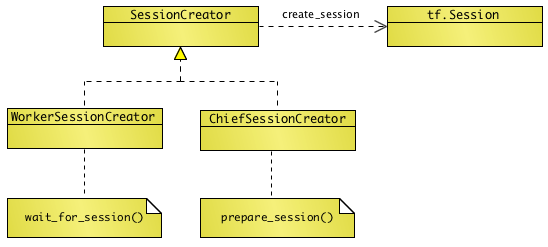
\includegraphics[width=0.9\textwidth]{figures/py-train-session-creator.png}
\caption{SessionManager}
 \label{fig:py-train-session-creator}
\end{figure}

\subsection{Scaffold}

当要构建一个模型训练,需要\code{init\_op}初始化变量;需要\code{Saver}周期性实施\ascii{Checkpoint};需要\code{ready\_op}查看一个模型是否已经初始化完毕;需要\code{summary\_op}搜集所有\ascii{Summary},用于训练过程的可视化。

一般地,在计算图中通过\code{GraphKey}标识了这些特殊的OP或对象,以便可以从计算图中检索出这些特殊的\ascii{OP}或对象。

在训练模型的特殊领域中,提供了一个基础工具库:\code{Scaffold},用于创建这些\ascii{OP}或对象的默认值,并添加到计算图的集合中,并且\code{Scaffold}提供了查询接口可以方便地获取到这些\ascii{OP}或对象。

可以通过调用\code{Scaffold.finalize}方法,如果对应的\ascii{OP}或对象为\code{None},则默认创建该类型的实例。最终冻结计算图,之后禁止再往图中增加节点。

\begin{leftbar}
\begin{python}
class Scaffold(object):
  def finalize(self):
    """Creates operations if needed and finalizes the graph."""
    
    # create init\_op
    if self._init_op is None:
      def default_init_op():
        return control_flow_ops.group(
            variables.global_variables_initializer(),
            resources.initialize_resources(
              resources.shared_resources()))
      self._init_op = Scaffold.get_or_default(
          'init_op',
          ops.GraphKeys.INIT_OP,
          default_init_op)

    # create ready\_op
    if self._ready_op is None:
      def default_ready_op():
        return array_ops.concat([
            variables.report_uninitialized_variables(),
            resources.report_uninitialized_resources()
        ], 0)
      self._ready_op = Scaffold.get_or_default(
          'ready_op', 
          ops.GraphKeys.READY_OP,
          default_ready_op)
    
    # create ready\_for\_local\_init\_op
    if self._ready_for_local_init_op is None:
      def default_ready_for_local_init_op():
        return variables.report_uninitialized_variables(
            variables.global_variables())
      self._ready_for_local_init_op = Scaffold.get_or_default(
          'ready_for_local_init_op',
          ops.GraphKeys.READY_FOR_LOCAL_INIT_OP,
          default_ready_for_local_init_op)
    
    # create local\_init\_op
    if self._local_init_op is None:
      def _default_local_init_op():
        return control_flow_ops.group(
            variables.local_variables_initializer(),
            lookup_ops.tables_initializer())
      self._local_init_op = Scaffold.get_or_default(
          'local_init_op',
          ops.GraphKeys.LOCAL_INIT_OP,
          _default_local_init_op)
    
    # create summary\_op
    if self._summary_op is None:
      self._summary_op = Scaffold.get_or_default(
          'summary_op',
          ops.GraphKeys.SUMMARY_OP,
          summary.merge_all)
    
    # create Saver
    if self._saver is None:
      self._saver = training_saver._get_saver_or_default()
    self._saver.build()

    ops.get_default_graph().finalize()
    return self
\end{python}
\end{leftbar}

从\code{finalize}的实现可以看出,以下\ascii{OP}完成的功能为:

\begin{enum}
  \eitem{\code{init\_op}: 完成所有全局变量和全局资源的初始化;}
  \eitem{\code{local\_init\_op}: 完成所有本地变量和表格的初始化;} 
  \eitem{\code{ready\_op}: 查看所有的全局变量和全局资源是否已经初始化了;否则报告未初始化的全局变量和全局资源的列表;}   
  \eitem{\code{ready\_for\_local\_init\_op}: 查看所有的本地变量和表格是否已经初始化了;否则报告未初始化的本地变量和表格的列表;}   
  \eitem{\code{summary\_op}: 汇总所有\ascii{Summary}的输出;}       
\end{enum}

其中,本地变量不能持久化到\ascii{Checkpoint}文件中;当然,也就不能从\ascii{Checkpoint}文件中恢复本地变量的值。

\subsection{初始化算法}

通过观测上面的\ascii{OP}的定义,理解\code{prepare\_session}模型初始化的完整语义便不是那么困难了。

\begin{leftbar}
\begin{python}
class SessionManager(object):
  def prepare_session(self,
                      master,
                      saver=None
                      checkpoint_filename=None
                      init_op=None,
                      init_feed_dict=None,
                      init_fn=None):
    """Creates a Session. Makes sure the model is ready."""

    def _restore_checkpoint():
      sess = session.Session(master)
      if not saver or not checkpoint_filename):
        return sess, False
      else:
        saver.restore(sess, checkpoint_filename)
        return sess, True

    def _try_run_init_op(sess):
      if init_op is not None:
        sess.run(init_op, feed_dict=init_feed_dict)
      if init_fn:
        init_fn(sess)
    
    sess, is_succ = self._restore_checkpoint()
    if not is_succ:
      _try_run_init_op(sess)
    self._try_run_local_init_op(sess)
    self._model_ready(sess)
    return sess
\end{python}
\end{leftbar}

其初始化算法非常简单。首先,尝试从\ascii{Checkpoint}文件中恢复(此处为了简化问题,省略了部分实现);如果失败,则调用\code{init\_op}和\code{init\_fn}完成全局变量和资源的初始化;然后,才能实施本地变量和表格的初始化;最后,验证所有全局变量和资源是否已经初始化了。

\begin{figure}[!htbp]
\centering
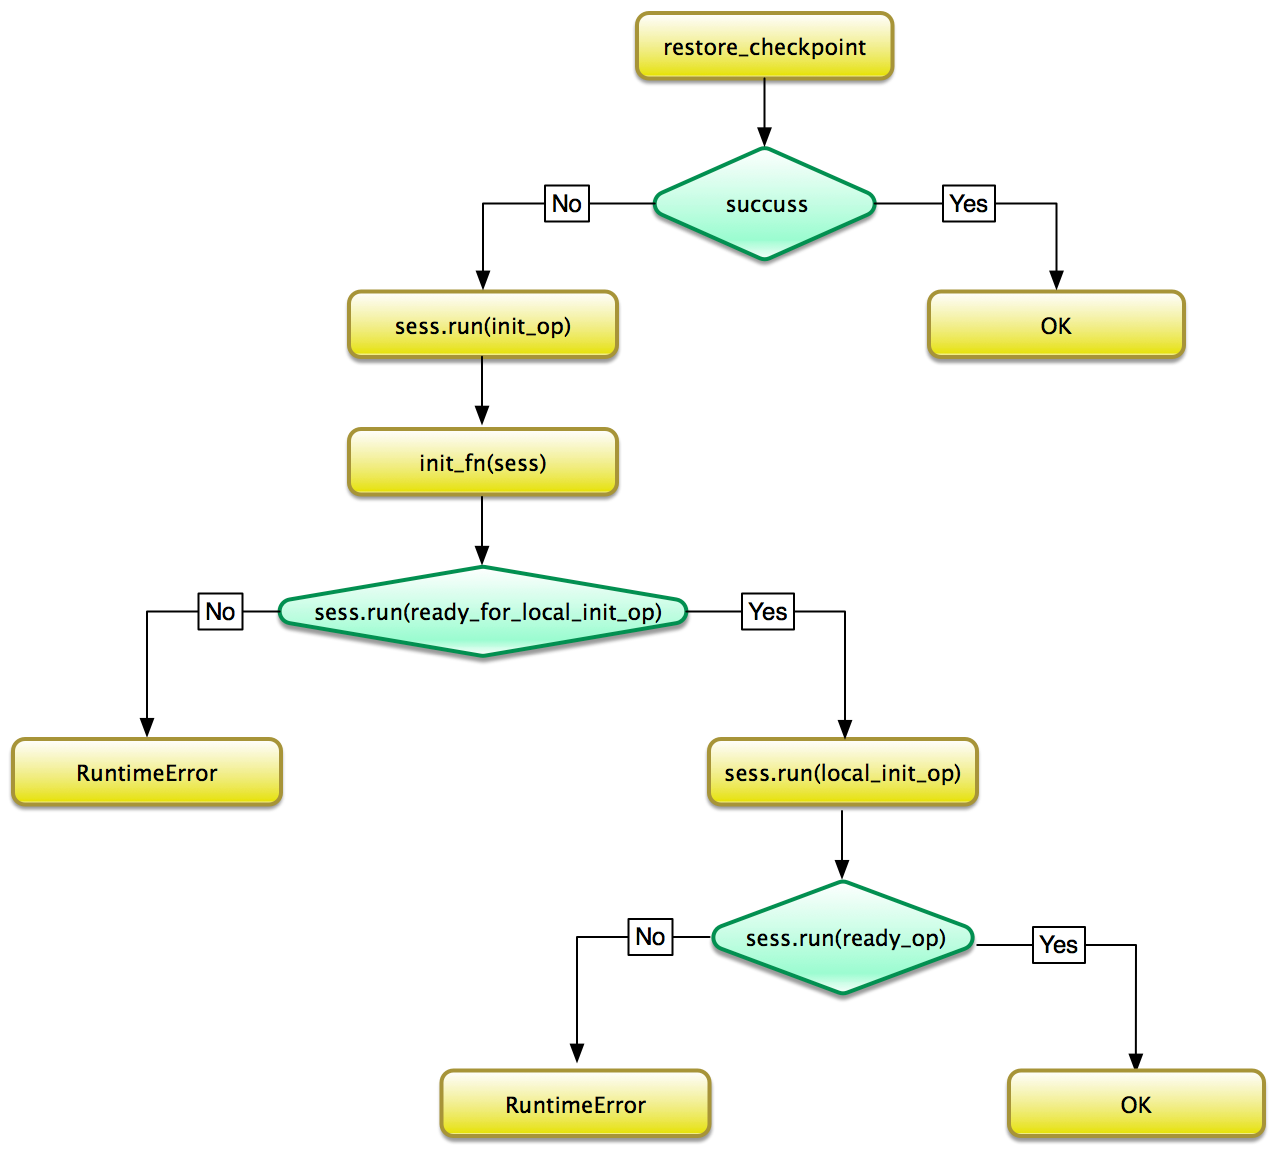
\includegraphics[width=0.9\textwidth]{figures/py-train-session-initialization-algo.png}
\caption{模型初始化算法}
 \label{fig:py-train-session-initialization-algo}
\end{figure}

\subsection{本地变量初始化}

对于非空的\code{local\_init\_op},必须等所有全局变量已经初始化完毕后才能进行初始化(通过调用\code{\_ready\_for\_local\_init\_op});否则,报告未初始化的全局变量列表到\code{msg}字段中。

也就是说,本地变量初始化在全局变量初始化之后,且本地变量不会持久化到\ascii{Checkpoint}文件中。

\begin{leftbar}
\begin{python}
class SessionManager(object):
  def _ready_for_local_init(self, sess):
    """Checks if the model is ready to run local_init_op.
    """
    return _ready(self._ready_for_local_init_op, sess,
                  "Model not ready for local init")

  def _try_run_local_init_op(self, sess):
    """Tries to run _local_init_op, if not None, 
       and is ready for local init.
    """
    if not self._local_init_op:
      return True, None:
    
    is_ready, msg = self._ready_for_local_init(sess)
    if is_ready:
      sess.run(self._local_init_op)
      return True, None
    else:
      return False, msg
\end{python}
\end{leftbar}

\subsection{验证模型}

最后,通过执行\code{\_ready\_op},查看所有全局变量和全局资源是否都已经初始化了;否则,报告未初始化的变量列表到\code{msg}字段中。

\begin{leftbar}
\begin{python}
class SessionManager(object):
  def _model_ready(self, sess):
    """Checks if the model is ready or not.
    """
    return _ready(self._ready_op, sess, "Model not ready")
\end{python}
\end{leftbar}

其中,\code{\_ready}使用函数,用于运行相应的\code{ready\_op},查看相应的变量或资源是否完成初始化。

\begin{leftbar}
\begin{python}
def _ready(op, sess, msg):
  """Checks if the model is ready or not, as determined by op.
  """
  if op is None:
    return True, None

  ready_value = sess.run(op)
  if (ready_value.size == 0):
    return True, None
  else:
    uninitialized_vars = ", ".join(
        [i.decode("utf-8") for i in ready_value])
    return False, "initialized vars: " + uninitialized_vars
\end{python}
\end{leftbar}

\end{content}

\section{异常安全}

\begin{content}

一般地,常常使用\code{with}的上下文管理器,实现\code{MonitoredSession}的异常安全和资源安全释放。

\subsection{上下文管理器}

当退出\code{with}语句后,将停止运行所有\code{QueueRunner}实例,并实现\code{tf.Session}的安全关闭。

\begin{leftbar}
\begin{python}
class _MonitoredSession(object):
  def __exit__(self, exception_type, exception_value, traceback):
    if exception_type in [errors.OutOfRangeError, StopIteration]:
      exception_type = None
    self._close_internal(exception_type)
    return exception_type is None
  
  def _close_internal(self, exception_type=None):
    try:
      if not exception_type:
        for h in self._hooks:
          h.end(self.tf_sess)
    finally:
      try:
        self._sess.close()
      finally:
        self._sess = None
        self.tf_sess = None
        self.coord = None  
\end{python}
\end{leftbar}

特殊地,当发生\code{OutOfRangeError}或\code{StopIteration},则认为正常终止,忽视该异常。如果抛出了其它类型的异常,则不会调用\code{end}的回调钩子。

\subsection{停止QueueRunner}

另外,当执行\code{self.\_sess.close()},最终将调用\code{\_CoordinatedSession}的\code{close}方法。通过调用\code{coord.request\_stop}通知所有\code{QueueRunner}实例停止运行,并且通过调用\code{coord.join}方法等待所有\code{QueueRunner}实例运行完毕。

\begin{leftbar}
\begin{python}
class _CoordinatedSession(_WrappedSession):
  def close(self):
    self._coord.request_stop()
    try:
      self._coord.join()
    finally:
      try:
        _WrappedSession.close(self)
      except Exception:
        pass
\end{python}
\end{leftbar}

\end{content}

\section{回调钩子}

\begin{content}

可以通过定制\code{SessionRunHook},实现对\code{MonitorSession}生命周期过程的监听和管理。

\begin{leftbar}
\begin{python}
class SessionRunHook(object):
  def begin(self):
    pass

  def after_create_session(self, session, coord):
    pass

  def before_run(self, run_context):
    return None

  def after_run(self, run_context, run_values):
    pass

  def end(self, session):
    pass
\end{python}
\end{leftbar}

其中,最常见的\code{Hook}包括:

\begin{enum}
  \eitem{\code{CheckpointSaverHook}:周期性地\ascii{Checkpoint};}
  \eitem{\code{SummarySaverHook}:周期性地运行\ascii{Summary};} 
  \eitem{\code{StepCounterHook}:周期性地统计每秒运行的\ascii{Step}数目。}   
\end{enum}

\begin{figure}[!htbp]
\centering
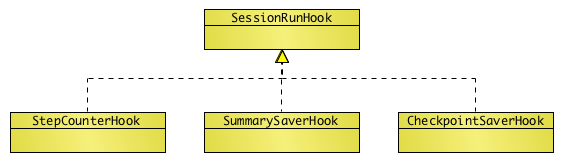
\includegraphics[width=0.9\textwidth]{figures/py-train-session-run-hook.png}
\caption{SessionRunHook}
 \label{fig:py-train-session-run-hook}
\end{figure}

\end{content}








%%%%%%%%%%%%%%%%%%%%%%
\backmatter
%\listoffigures
%\myclearpage
%\listoftables
%\myclearpage

%\include{contents/appendix}	

% %% 加入参考文献支持
% \bibliographystyle{alpha}
% \bibliography{contents/ref}

\end{document}
%%%% 正文部分结束
%%%%%%%%------------------------------------------------------------------------
